\documentclass[times, utf8, zavrsni]{fer}
\usepackage{booktabs}
\usepackage{pdfpages}
\usepackage{placeins}
\usepackage{verbatimbox}
\usepackage{listings}
\usepackage{amsmath}
\usepackage{graphicx} % \scalebox
\usepackage{environ}
\NewEnviron{myequation}{%
\begin{equation}
\scalebox{1.5}{$\BODY$}
\end{equation}
}


\begin{document}

% TODO: Navedite broj rada.
\thesisnumber{874}

% TODO: Navedite naslov rada.
\title{Aplikacija za praćenje rangiranja sveučilišta prema Šangajskoj listi}

% TODO: Navedite vaše ime i prezime.
\author{Ivan Bilobrk}

\maketitle

% Ispis stranice s napomenom o umetanju izvornika rada. Uklonite naredbu \izvornik ako želite izbaciti tu stranicu.

\includepdf[pages=-]{zadatak.pdf}

% Dodavanje zahvale ili prazne stranice. Ako ne želite dodati zahvalu, naredbu ostavite radi prazne stranice.
\zahvala{}

\tableofcontents

\chapter{Uvod}
U svijetu postoji više od 25000 sveučilišta. Svako od njih trudi se imati što bolje predavače, kvalitetniju nastavu, puno znanstvenih radova, sudjelovanja na konferencijama,
objava u časopisima te drugih raznih uspjeha. Sveučilištima je teško uskladiti svoju organizaciju bez neke povratne informacije o svojim uspjesima. Upravo zbog toga napravljene su razne
rang liste koje svakom sveučilištu pridružuju neku numeričku vrijednost što omogućuje da se sveučilišta poredaju
odnosno da se rangiraju po uspješnosti. 
Na ovaj način svako sveučilište dobiva svoju poziciju 
koja može služiti kao mjerilo uspjeha, ukazati na potencijalne probleme na sveučilištu te tako omogućiti uvođenje promjena na sveučilištu kako bi 
na sljedećoj rang listi sveučilište bilo na nekoj višoj poziciji.\\ Neke od organizacija koje objavljuju rang liste sveučilišta su: Times Higher Education, Round University Ranking,
U.S. News, i Shanghai Ranking. U kontekstu ovog \\završnog rada, proučava se način rangiranja Shanghai Ranking sustava. \\ Shanghai Ranking objavljuje jednom godišnje dvije 
rang liste. Prva rangira sveučilišta neovisno o područjima istraživanja i zove se Academic Ranking of World Universities (ARWU). ARWU se objavljuje od 2003. godine i  
temelji se na 6 indikatora uspjeha. Rangira više od 2000 sveučilišta, a samo najboljih 1000 objavi na službenoj stranici. Za ovaj završni rad,
zanimljivija rang lista je Global Ranking of Academic Subjects
(GRAS) jer rangira sveučilišta u nekom području istraživanja. Ovu rang listu \\Shanghai Ranking objavljuje od 2009. godine. Zadnja rang lista, 2022. godine, uključivala je više od 1800 sveučilišta 
u više od 96 zemalja u 54 područja istraživanja. Fakultet elektrotehnike i računarstva u Zagrebu (FER) dio je Sveučilišta u Zagrebu te su rang liste u području 
računarske znanosti i inženjerstva \engl {Computer Science \\\& Engineering (CSE)} i elektrotehnike \engl {Electrical \& Electronic Engineering (EEE)} u središtu istraživanja
ovog završnog rada. Problem tih rang lista 
na \\Shanghai Ranking stranici je taj što objavljuju samo prvih 500 najboljih sveučilišta u tim područjima što znači da se rang Sveučilišta u Zagrebu u kategorijama
CSE i EEE ne može ni provjeriti. 
Ovaj završni rad bavi se izradom aplikacije koja će prikupljati podatke o sveučilištima na isti način kao i Shanghai Ranking, ali uz iznimku da nema ograničenja na 
broj sveučilišta koja se mogu pojaviti na konačnoj rang listi. Na ovaj način Sveučilište u Zagrebu, a i FER, moći će pratiti svoj napredak iz godine u godinu te raditi određene 
promjene kako bi im se pozicija na rang listi poboljšala. 

\chapter{Shanghai Ranking metodologija}
Shanghai Ranking Global Ranking of Academic Subjects (GRAS) objavljuje se svake godine i temelji se na podatcima kroz pet godina.
Ako  se promatra rang listu za neku godinu $x$,
donja granica godina za podatke je $x-6$, a donja granica je $x-2$. Tako primjerice, rang lista za 2022. godinu temelji se na podatcima od 2016. do 2020. godine, uključivo.

\section{Indikatori za izradu rang liste}
\label{indikatori}
Global Ranking of Academic Subjects (GRAS) računa se na temelju pet indikatora, a to su: Q1, CNCI, IC, \emph{Top} i \emph{Award}.
\\ \\\textbf{Q1} indikator predstavlja broj radova koje je institucija objavila u nekom području \\istraživanja 
u časopisima s Q1 kvartilom faktora utjecaja na časopis tijekom nekog \\vremenskog razdoblja.   
\\ \\\textbf{CNCI} indikator (\emph{Category Normalized Citation Impact}) omjer je citiranosti \\objavljenih radova i prosječnih citiranosti 
radova u istoj kategoriji, iste godine i iste vrste publikacije u časopisu, od strane sveučilišta u određenom području tijekom relevantnog razdoblja.
CNCI vrijednosti manje od 1 znače da je citiranost sveučilišta manja od prosjeka, vrijednost 1 znači da je citiranost prosječna, a vrijednosti veće od
1 znače da je citiranost sveučilišta veća od prosjeka.
\\ \\\textbf{IC} indikator (\emph{International Collaboration}) predstavlja koliko međunarodnih suradnja sveučilište u nekom području istraživanja ima.
Točna vrijednost indikatora dobije se kao omjer broja publikacija koje su pronađene u najmanje dvije različite zemlje 
u \\odnosu na adresu autora prema ukupnom broju publikacija iz odgovarajućeg područja istraživanja za instituciju tijekom relevantnog razdoblja.
\\ \\\textbf{\emph{Top}} indikator predstavlja broj radova objavljenih u najboljim časopisima iz nekog područja za instituciju u nekom vremenskom razdoblju. 
Najbolje časopise nominiraju \\istaknuti znanstvenici kroz Shanghai Ranking anketu o akademskoj izvrsnosti. \\Iznimka je područje CSE 
jer se za izračun ovog indikatora ne gleda broj radova \\objavljenih u časopisima nego se gleda broj radova predstavljenih na 31 odabranoj \\konferenciji.
Konferencije također biraju istaknuti znanstvenici kroz Shanghai \\Ranking anketu.
\\ \\\textbf{\emph{Award}} indikator predstavlja broj osoba sveučilišta koje je dobilo značajnu nagradu iz nekog područja istraživanja. Značajne nagrade 
biraju se također putem AES-a. Značajna nagrada za područje CSE je Turingova 
nagrada, a za područje EEE je IEEE Medal of Honor.
Kako bi dobitak nagrade išao u korist sveučilištu, osoba koje je dobila nagradu morala je u trenutku dobitka nagrade raditi puno radno vrijeme na 
tom sveučilištu, a ako  je osoba u trenutku dobitka nagrade bila povezana s više sveučilišta ili drugih institucija, svakoj ustanovi se pridjeljuje
recipročan broj broja sveučilišta. Tako na primjer, ako je osoba bila povezana s 3 ustanove, svakoj od njih se pridjeljuje $1/3$, a ako je bila 
povezana samo s jednom ustanovom pridjeljuje se toj ustanovi $1$. 
Vrijeme dobitka nagrade također igra ulogu jer u obzir dolaze nagrade dodijeljene unazad 4 desetljeća od gornje granice godina za koje se promatraju podatci.
Ako se promatra rang lista za 2022. godinu, onda je gornja granica godine za podatke 2020. Svakom desetljeću pridjeljuju se različite težine 
s kojima se onda množi \\prethodno dobiveni broj. Desetljeću najbližem sadašnjosti pridjeljuje se težina 1, a svim ostalima smanjuje se za 0.25.
Ukupna vrijednost indikatora dobije se zbrajanjem pojedinih vrijednosti za neko sveučilište u nekom području.

\begin{table}[htb]
    \caption{Primjer težina za indikator \emph{Award} za rang listu 2022. godine}
        \label{tbl:konstante2}
        \centering
        \begin{tabular}{cccc} \hline
        2011.-2020. & 2001.-2010. & 1991.-2000. & 1981.-1990.\\ \hline
        1&0.75&0.5&0.25\\
        \end{tabular}
        \end{table}    
        \FloatBarrier
\subsection{Izvori za prikupljanje podataka}        
Podatke za izračun svih 5 vrijednosti indikatora, osim indikatora \emph{Award}, prikupljaju se s baza InCites i Web of Science (WoS). 
Podatci za indikator \emph{Award} mogu se pronaći na službenim stranicama koje objavljuju dobitnike nagrada za neko područje.
Za \\\\\emph{Computer Science \& Engineering} (CSE) to je stranica A.M. Turing Award, a za \emph{\\Electrical \& Electronic Engineering} (EEE) IEEE Awards.

\section{Minimalni broj publikacija} Kako bi sveučilište ušlo na rang listu za područja CSE i EEE mora imati minimalno 150 publikacija koje su vidljive 
na bazama WoS i InCites.
\\ \section{Preslikavanje područja istraživanja}Kako bi se podatci uspješno prikupili s navedenih baza, potrebno je odabrati ispravno područje istraživanja jer preslikavanja nisu $1:1$.
\\\\U sljedećim tablicama vidi se kako izgledaju preslikavanja za područja CSE i EEE.

\begin{table}[htb]
    \caption{Preslikavanje za područje \emph{Computer Science \& Engineering} (CSE)}
    \label{tbl:konstante}
    \centering
    \begin{tabular}{ll} \hline
    Područje na Shanghai Ranking stranici & Područje na InCites i \\ & Web of Science (WoS) bazama\\ \hline
    \emph{Computer Science \& Engineering} & \emph{Computer Science, Information Systems} \\
    \emph{Computer Science \& Engineering} & \emph{Computer Science, Cybernetics} \\
    \emph{Computer Science \& Engineering} & \emph{Computer Science, Software Engineering} \\
    \emph{Computer Science \& Engineering} & \emph{Computer Science, Artificial Intelligence} \\
    \emph{Computer Science \& Engineering} & \emph{Computer Science, Hardware \& Architecture} \\
    \emph{Computer Science \& Engineering} & \emph{Computer Science, Theory \& Methods} \\
    \emph{Computer Science \& Engineering} & \emph{Computer Science, Interdisciplinary Applications} \\
    \end{tabular}
    \end{table}
    \FloatBarrier
    \hfil

\begin{table}[htb]
    \caption{Preslikavanje za područje Electrical \& Electronic Engineering (EEE)}
        \label{tbl:konstante1}
        \centering
        \begin{tabular}{ll} \hline
        Područje na Shanghai Ranking stranici & Područje na InCites i \\ & Web of Science (WoS) bazama\\ \hline
        \emph{Electrical \& Electronic Engineering} &  \emph{Engineering, Electrical \& Electronic}\\
        \emph{Electrical \& Electronic Engineering} &  \emph{Imaging Science \& Photographic Technology}\\
        \end{tabular}
        \end{table}    
        \FloatBarrier
\newpage
\section{Računanje ukupnog rezultata sveučilišta}
Uz vrijednosti svih indikatora za neko sveučilište ukupna brojčana vrijednost prema kojoj se sveučilišta rangiraju računa 
se na sljedeći način:
\\Svaki od indikatora osim CNCI-ja podijeli se s najvećom vrijednosti indikatora od svih sveučilišta, iz tog broja izvadi se
drugi korijen te dobiveni broj pomnoži se s težinom tog indikatora.
Na kraju dobivene vrijednosti se sumiraju.
\\
\\ Izračun vrijednosti koja se pridjeljuje nekom indikatoru: 
\begin{align}
    \sqrt[\leftroot{-2}]{\frac{vrijednost \; indikatora}{max(indikator)}} \; * tezina(indikator) \label{eq:a}
\end{align}
\\ Indikator CNCI je poseban te se njemu pridjeljuje sljedeća vrijednost: \\ 
\begin{align}
    \sqrt[\leftroot{-2}]{\frac{vrijednost \; CNCI \; indikatora}{min(2*average(CNCI), max(CNCI))}} \; * tezina(CNCI) \label{eq:b}
    \end{align}
\\ Ako je vrijednost CNCI indikatora veća od vrijednosti brojnika u izrazu \ref{eq:b} onda se sveučilištu automatski pridjeljuje vrijednost 100.

\begin{table}[htb]
    \caption{Težine s kojima se vrijednosti pridružene indikatorima množe}
        \label{tbl:konstante3}
        \centering
        \begin{tabular}{ccccc} \hline
        Q1 & CNCI & IC & \emph{Top} & \emph{Award} \\ \hline
        100&100&20&100&100\\
        \end{tabular}
        \end{table}    
        \FloatBarrier

\subsection{Primjer izračuna vrijednosti koje se vežu uz indikatore}
\label{racunanje}
U sljedećem dijelu prikazan je primjer izračuna vrijednosti koje se vežu uz indikatore za sveučilište University of California, Berkeley koje je 2022. godine bilo prvo na 
Shanghai Ranking rang listi u području EEE.
Period tijekom kojeg se uzimaju podatci je od 2016. godine do 2020. godine.
\\
\\ \underline{Vrijednost Q1:} 
\\ Pretraživanjem InCites baze saznaje se da navedeno sveučilište ima vrijednost indikatora Q1 603. Najveća vrijednost Q1 indikatora u tom razdoblju iznosi 3285.
Vrijednost koja se veže za Q1 indikator iznosi;  \; $\sqrt[\leftroot{-2}]{\frac{603}{3285}} \; * 100 = 42.8$
\\
\\ \underline{Vrijednost CNCI:} 
\\ Pretraživanjem InCites baze saznaje se da navedeno sveučilište ima vrijednost indikatora CNCI 1.71. Najveća vrijednost CNCI indikatora u tom razdoblju iznosi 4.13.
Kako je riječ o indikatoru CNCI u obzir se još mora uzeti i dvostruka prosječna vrijednost svih CNCI vrijednosti, a to je 2.27.
Vrijednost koja se veže za CNCI indikator iznosi: \; \\ $\sqrt[\leftroot{-2}]{\frac{1.71}{min(2.27, 4.13)}} \; * 100 = 86.8$
\\
\\ \underline{Vrijednost IC:} 
\\ Pretraživanjem InCites baze saznaje se da navedeno sveučilište ima vrijednost indikatora IC 57.18. Najveća vrijednost IC indikatora u tom razdoblju iznosi 97.15.
\\Vrijednost koja se veže za IC indikator iznosi: \; \\ $\sqrt[\leftroot{-2}]{\frac{57.18}{97.15}} \; * 20 = 15.3$
\\
\\ \underline{Vrijednost \emph{Top}:} 
\\ Pretraživanjem InCites baze saznaje se da navedeno sveučilište ima vrijednost indikatora \emph{Top} 25. Najveća vrijednost \emph{Top} indikatora u tom razdoblju iznosi 25.
Vrijednost koja se veže za \emph{Top} indikator iznosi: \; \\ $\sqrt[\leftroot{-2}]{\frac{25}{25}} \; * 100 = 100$
\\
\\ \underline{Vrijednost \emph{Award}:} 
\\ Pretraživanjem stranice IEEE Awards saznaje se da je navedeno sveučilište osvojilo nagradu IEEE Medal of Honor sljedećih godina: 1985., 1995., 1998., 2020. Kako je 
svake godine nagradu osvojila uvijek jedna osoba koja nije bila vezana za nijednu drugu ustanovu te je u vrijeme dobitka nagrade
radila puno radno vrijeme na tom sveučilištu, vrijednost 
indikatora \emph{Award} je $1*0.25+1*0.5+1*0.5+1*1 = 2.25$ (u obzir se uzimaju težine koje se vežu za godinu osvajanja nagrade). Najveća vrijednost 
indikatora \emph{Award} u tom razdoblju iznosi 3. Vrijednost koja se veže za \emph{Award} indikator iznosi: \; \\ $\sqrt[\leftroot{-2}]{\frac{2.25}{3}} \; * 100 = 86.6$
\\\\Jednom kada se izračunaju sve vrijednosti koje se vežu za pojedine indikatore,
ukupan rezultat sveučilišta University of California, Berkeley u 2022. godini dobije se zbrajanjem tih vrijednosti: $42.8+86.8+15.3+100+86.6 = 331.5$.
\section{Odstupanje procijenjenih i Shanghai Ranking vrijednosti indikatora}
Izračun vrijednosti koje se vežu uz indikatore kako je opisano u odjeljku 2.4.1 ne daje uvijek podatke koji se u potpunosti poklapaju s onima na 
Shanghai Ranking stranici.
\\Odstupanja proizlaze iz toga što je Shanghai Ranking rang lista za neku godinu fiksna, ne ažurira se novim podatcima, te iz toga što za pojedine 
indikatore nije u potpunosti jasno kako se računaju. \\Kada se pretražuju radovi sveučilišta
kroz InCites i WoS baze podataka uvijek se dobivaju najnoviji podatci za koje je moguće da su se promijenili od trenutka kada se računala Shanghai Ranking rang lista za neku godinu.
Primjer je indikator CNCI koji se temelji na broju citiranosti radova nekog sveučilišta. Moguće je da se neki rad citirao tek nakon što je Shanghai rang lista objavljena. Sveučilište uz 
koje se veže taj rad će na Shanghai Ranking rang listi imati manju vrijednost indikatora CNCI nego na procijenjenoj rang listi koja se temelji na novijim podatcima. 
Moguća situacija je i da su radovi tek nakon objave Shanghai Ranking rang liste za neku godinu uvršteni pod kategoriju međunarodnih suradnja što uzrokuje odstupanje 
indikatora IC. Ulogu također igra i zaokruživanje brojčanih vrijednosti, a postupak zaokruživanja na stranici Shanghai Ranking nije naveden.
\\Kako bi se dobio dojam odstupanja, prikupljeni su podatci prvih 100 sveučilišta sa Shanghai Ranking stranice za rang liste 2022. i 2021. godine u područjima CSE i EEE. 
Rezultati analize razlika procijenjenih i stvarnih vrijednosti vidljivi su na grafovima \ref{fig:graf2022} i \ref{fig:graf2021}. Postotna odstupanja računaju se prema sljedećem izrazu:
\begin{myequation}%
    \frac{|Shanghai\_Ranking\_vrijednost - procijenjena\_vrijednost|}{\frac{Shanghai\_Ranking\_vrijednost + procijenjena\_vrijednost}{2}}*100.
    \end{myequation}
\begin{figure}[htb]
    \centering
    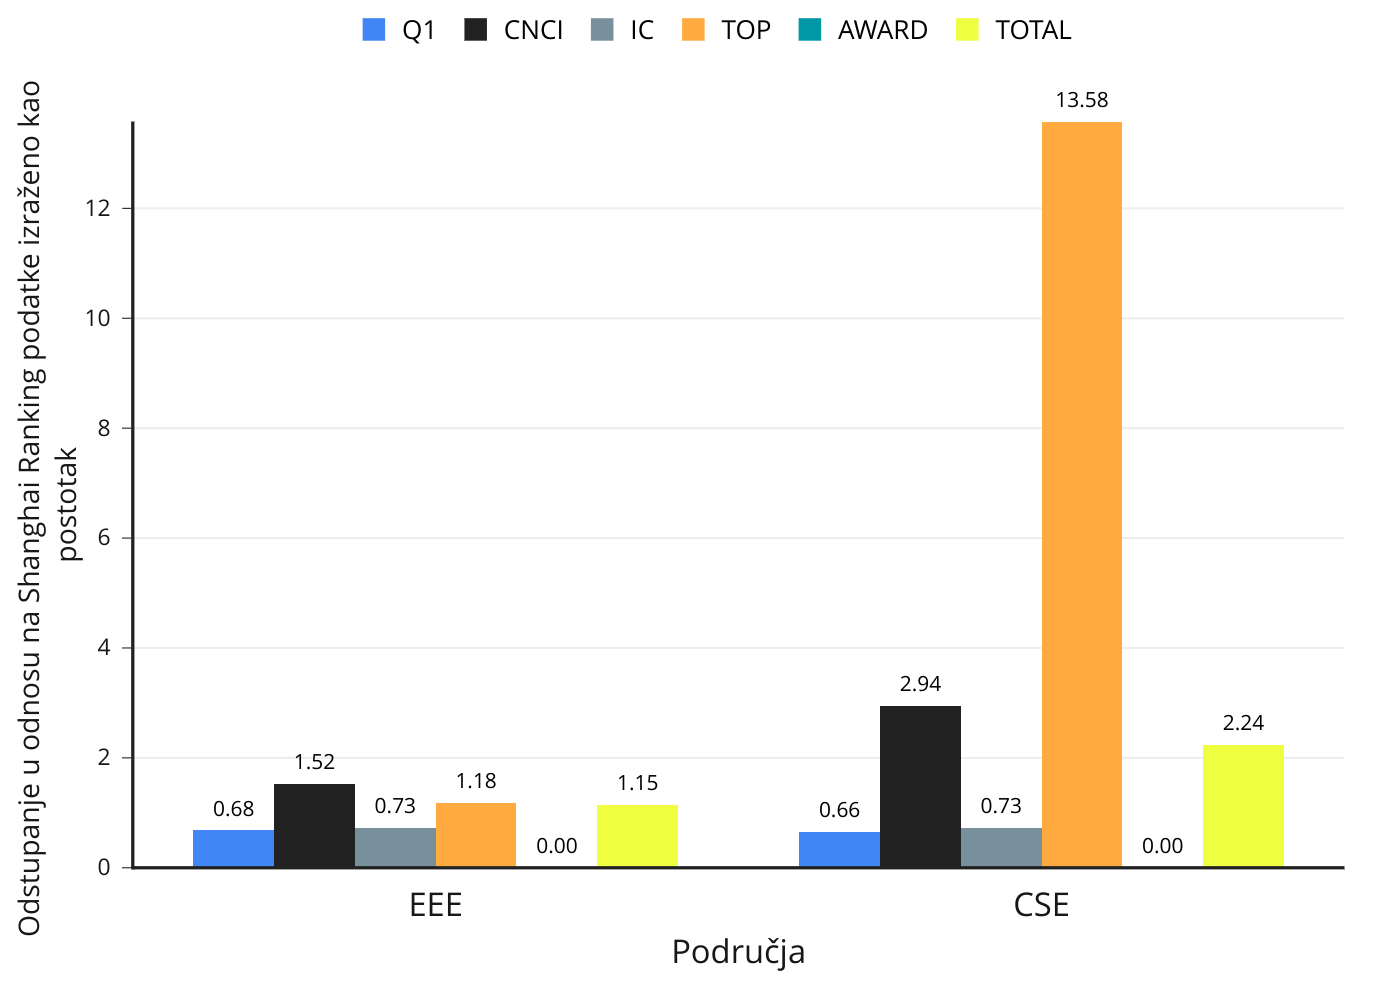
\includegraphics[scale=0.25]{EEE2022.png}
    \caption{Grafički prikaz odstupanja procijenjenih vrijednosti indikatora i ukupne vrijednosti \engl{total} za 2022. godinu gdje se odstupanje, izraženo kao postotak, za 
    neko sveučilište računa prema izrazu 2.3, a na grafu su prikazane prosječne vrijednosti svih odstupanja pojedinih podataka.}
    \label{fig:graf2022}
    \end{figure}
    \FloatBarrier

    \begin{figure}[htb]
        \centering
        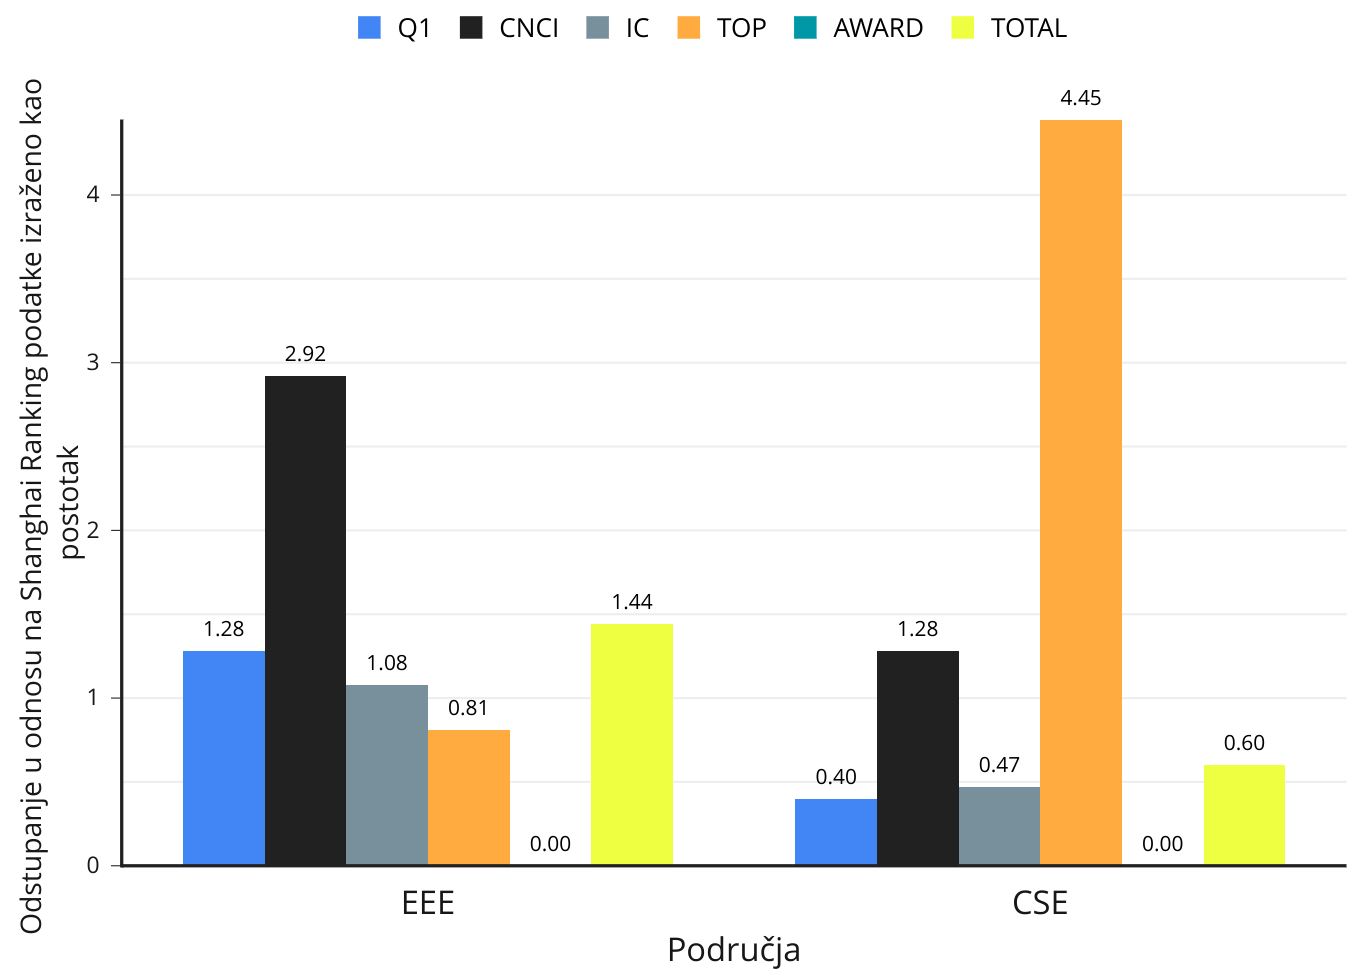
\includegraphics[scale=0.25]{graf2021.png}
        \caption{Grafički prikaz odstupanja procijenjenih vrijednosti indikatora i ukupne vrijednosti \engl{total} za 2021. godinu gdje se odstupanje, izraženo kao postotak, za 
        neko sveučilište računa prema izrazu 2.3, a na grafu su prikazane prosječne vrijednosti svih odstupanja pojedinih podataka.}
        \label{fig:graf2021}
        \end{figure}   
        \FloatBarrier 

Na temelju analize vidi se da je indikator \emph{Top} posebno problematičan za područje CSE. Iako je popis imena svih konferencija koje se uzimaju u obzir
prilikom računanja naveden, imena sa Shanghai Ranking stranice razlikuju se od onih dostupnih 
na InCites i WoS stranicama te pretragom konferencija za određenu godinu dobiju se višestruki rezultati iz kojih nije sasvim jasno koji odabrati. Za područje EEE procjena 
indikatora \emph{Top} je manje pogrešna jer se računa na temelju radova objavljenih u dvama časopisima te prilikom pretrage InCites i WoS baze dobiju se jako precizni podatci.
\\Za indikator \emph{Award} odstupanja nema jer su podatci za izračun njegove vrijednosti ručno uneseni u bazu podataka.
\\Osim vrijednosti indikatora i ukupne sume \engl{total} usporediti se mogu i pozicije na procijenjenoj i stvarnoj Shanghai Ranking rang listi.
Na svakoj Shanghai Ranking listi za područja CSE i EEE nalazi se 500 sveučilišta. Samo prvih 50 ima dodijeljenu točnu poziciju, dok se ostale pozicije određuju
otprilike te sveučilištima nije dodijeljena točna pozicija nego interval pozicija. Na grafovima \ref{fig:pozicije2021} i \ref{fig:pozicije2022}
prikazana je \\uspješnost procjene pozicije na rang listi. U okviru ove analize, 
pozicija se smatra uspješno procijenjenom ako je apsolutna razlika procijenjene i Shanghai Ranking pozicije manja od 4. Ako je riječ o intervalu pozicija, 
pozicija se smatra uspješno procijenjenom ako se nalazi unutar intervala ili na udaljenosti manjoj od 4 od gornje ili donje granice intervala. Kriteriji uspješnosti 
procjene pozicija su smanjeni jer ih je teško ispravno procijeniti. Nekad i najmanje razlike ukupne sume bodova uzrokuju veliku razliku ranga na listi. 
Bolja procjena vrijednosti indikatora \emph{Top} za područje EEE sada dolazi do izražaja jer su procjene pozicije bolje u odnosu na područje CSE.
\\Kako bi korisnik lakše usporedio procijenjene i stvarne Shanghai Ranking rang liste, u aplikaciji je dostupna opcija postavljanja \engl{upload} 
stvarnih Shanghai Ranking podataka. Stranica koja ima tu funkcionalnost opisana je u dijelu 6.4. Postavljanjem stvarnih Shanghai Ranking podataka na dnu svake stranice gdje se prikazuje
rang lista dotupna je ocjena uspješnosti procjene pozicija što je ustvari zadnji stupac na grafovima \ref{fig:pozicije2021} i \ref{fig:pozicije2022}. Osim ocjene procjene pozicija, 
mogu se usporediti i vrijednosti svih indikatora te ukupne sume bodova na stranici opisanoj u dijelu 6.3.
\begin{figure}[htb]
    \centering
    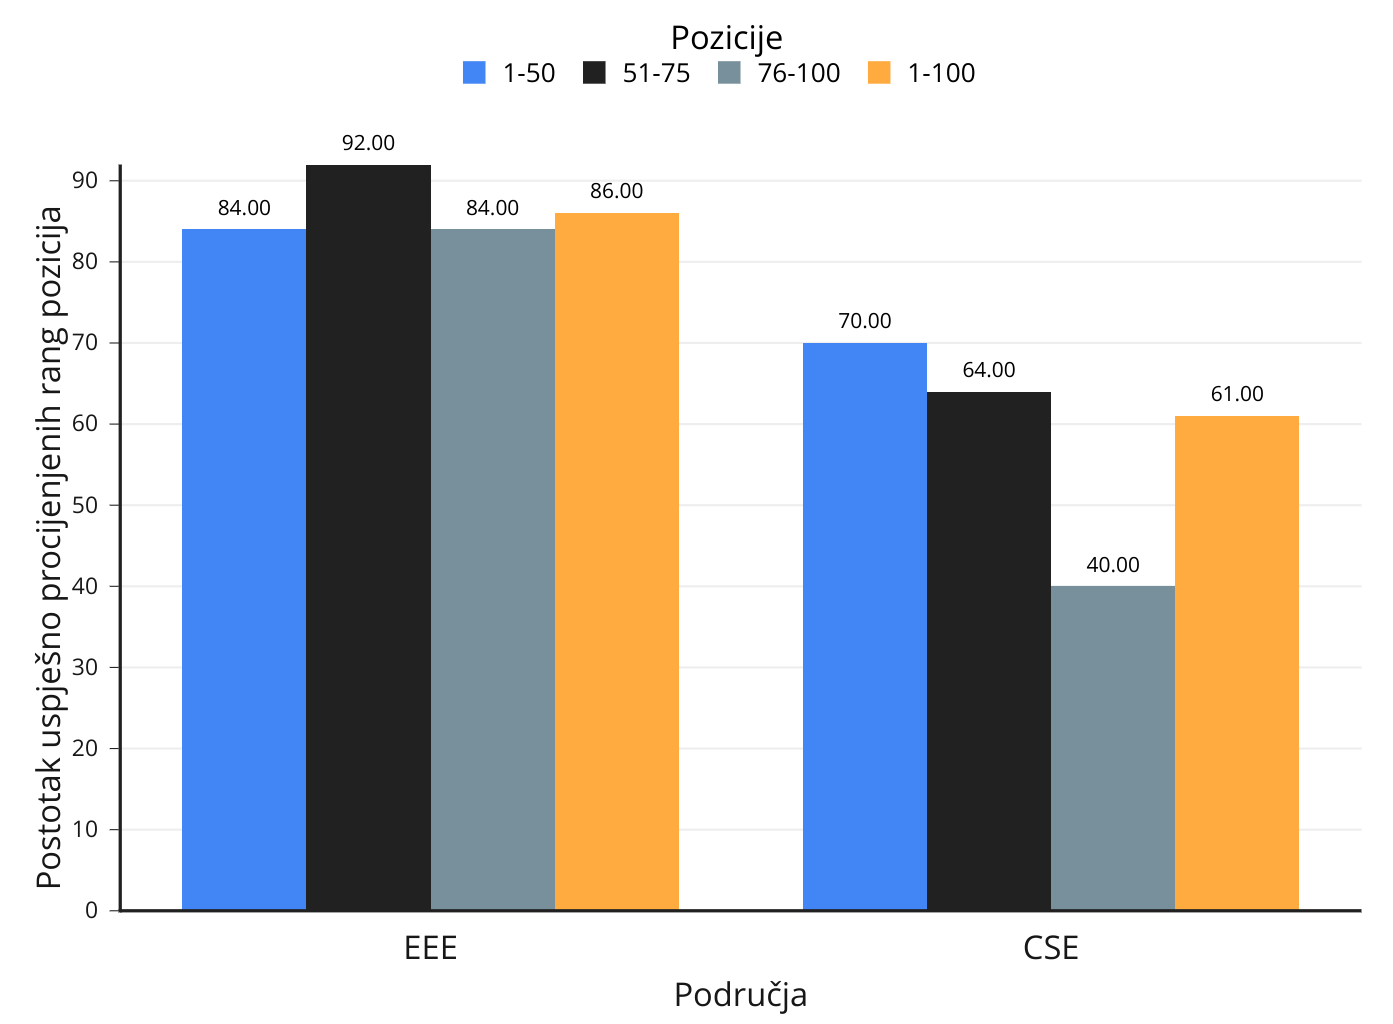
\includegraphics[scale=0.21]{pozicije2021.png}
    \caption{Grafički prikaz odstupanja procijenjenih vrijednosti pozicija za 2021. godinu gdje se pozicija smatra uspješno procijenjenom ako se nalazi 
    na udaljenosti manjoj od 4 od stvarne pozicije na Shanghai Ranking stranici. Postotno odstupanje pozicija pojedinih sveučilišta računa se prema izrazu 2.3, a 
    na grafu su prikazane prosječne vrijednosti odstupanja pozicija prvih 100 sveučilišta. Prvih 100 pozicija podijeljeno je na 4 intervala kao i na Shanghai \\Ranking stranici.}
    \label{fig:pozicije2021}
    \end{figure} 
    \begin{figure}[htb]
        \centering
        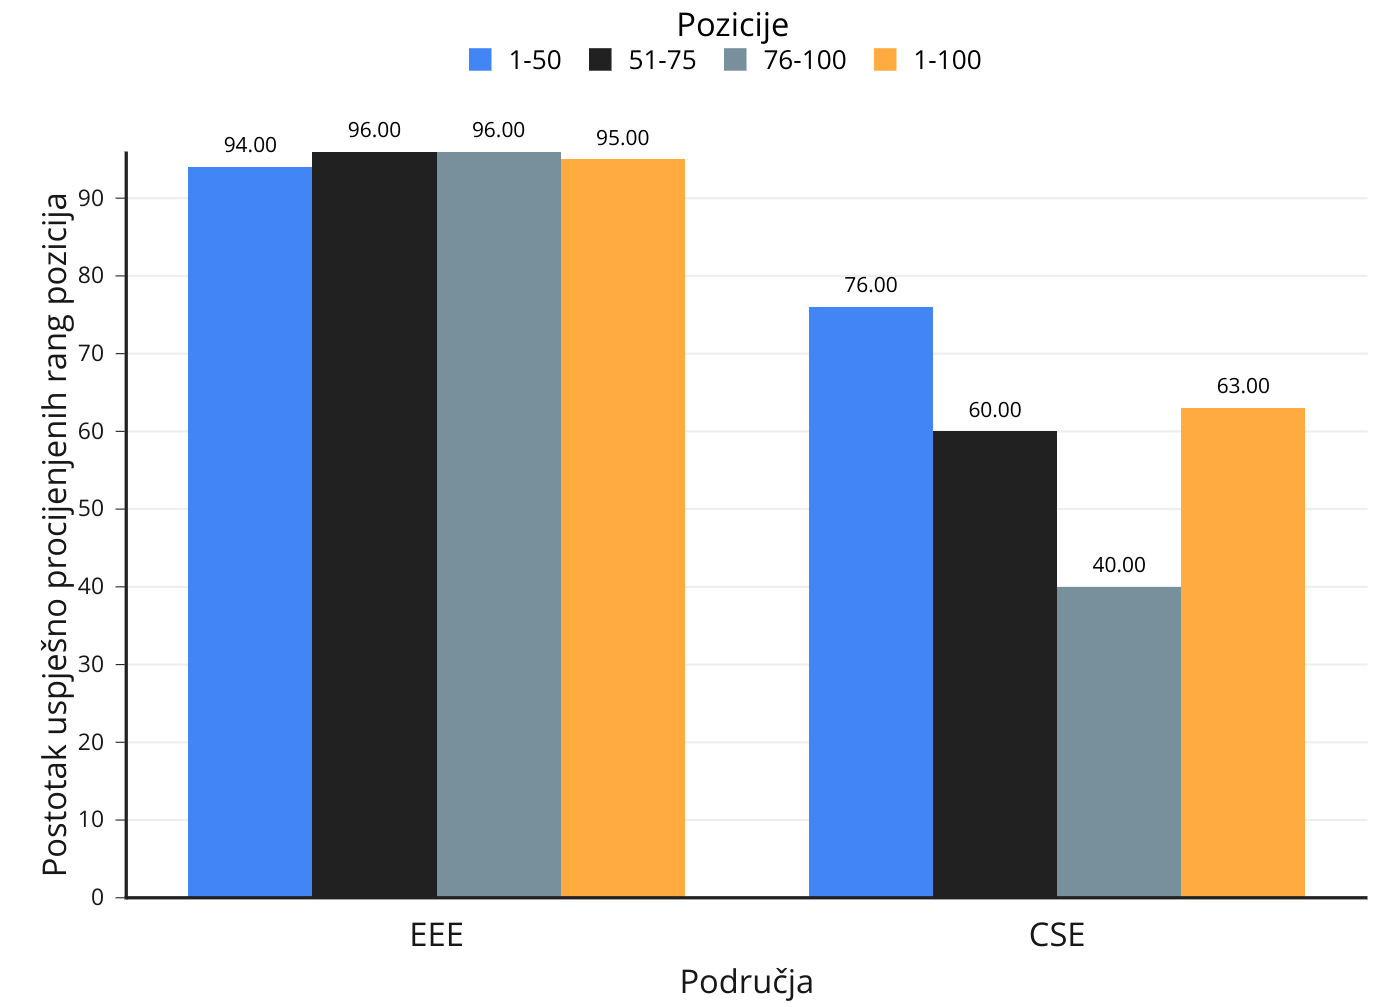
\includegraphics[scale=0.21]{pozicije2022.png}
        \caption{Grafički prikaz odstupanja procijenjenih vrijednosti pozicija za 2022. godinu gdje se pozicija smatra uspješno procijenjenom ako se nalazi 
        na udaljenosti manjoj od 4 od stvarne pozicije na Shanghai Ranking stranici. Postotno odstupanje pozicija pojedinih sveučilišta računa se prema izrazu 2.3, a 
        na grafu su prikazane prosječne vrijednosti odstupanja pozicija prvih 100 sveučilišta. Prvih 100 pozicija podijeljeno je na 4 intervala kao i na Shanghai \\Ranking stranici.}
        \label{fig:pozicije2022}
        \end{figure}   


\chapter{Zahtjevi aplikacije}
\section{Funkcionalni zahtjevi}
Funkcionalni zahtjevi predstavljaju sve usluge koje programski proizvod mora pružiti korisnicima te definiraju kako sustav reagira na određene ulazne poticaje.
\\ Aktori ovog programskog sustava su korisnici, React web grafičko sučelje, Node.js poslužitelj, PostgreSQL baza podataka, skupljač podataka potrebnih za rangiranje, 
\\InCites i WoS baze podataka.
\\
\\Korisnici mogu:

a) pregledati procijenjene rang liste sveučilišta za određenu godinu u područjima CSE i EEE

b) pregledati vrijednosti svih indikatora nekog sveučilišta pomoću kojih se računa procjena ranga za željeno područje i godinu

c) usporediti vrijednosti Shanghai Ranking sustava s procijenjenim vrijednostima za sva sveučilišta u nekom području i za neku godinu

d) pregledati uspješnost procjene rang liste za željeno područje i godinu

e) pregledati grafički prikaz promjene procjene vrijednosti indikatora i pozicije na rang listi sveučilišta u nekom području tijekom svih godina 
za koje se objavljuje rang lista, kao i pratiti napredak sveučilišta za trenutnu godinu
\\
\\React web grafičko sučelje može:

a) korisniku pružiti vizualni prikaz rang lista i podataka korištenih za rangiranje

b) dohvaćati podatke o rangiranju s poslužitelja
\\
\\Node.js poslužitelj:

a) nudi React web grafičkom sučelju krajnje točke potrebne za prikaz podataka korisniku.
\\\\
Skupljač podataka:

a) inicijalno puni PostgreSQL bazu podataka koristeći baze WoS i InCites s \\podatcima potrebnim za izračun procijenjene rang liste sveučilišta

b) svakih dva tjedna prikuplja podatke s baza WoS i InCites za procjenu ranga sveučilišta u trenutnoj godini
\\
\\PostgreSQL baza podataka:
 
a) pohranjuje vrijednosti indikatora potrebne za izračun procijenjene rang liste sveučilišta
\\
\begin{figure}[htb]
    \hspace*{-2cm}
    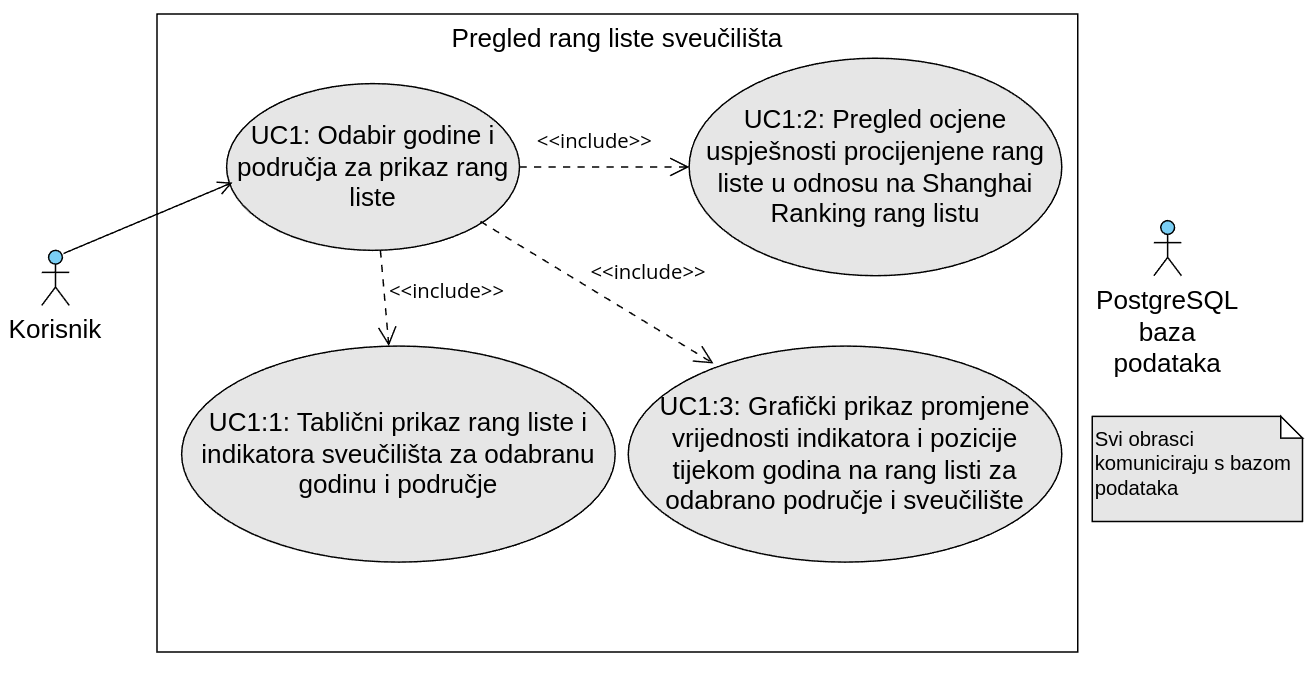
\includegraphics[scale=0.4]{slika1.png}
    \caption{Dijagram obrasca uporabe, korisnička funkcionalnost}
    \label{fig:korisnik}
    \end{figure}
\newpage
\section{Nefunkcionalni zahtjevi}
Nefunkcionalni zahtjevi opisuju koja svojstva sustav mora imati, a ne funkcionalnost koju pruža korisniku. Ova aplikacija mora:

a) biti robusna, otporna na pogreške i stabilna

b) omogućiti brzo i fluidno korisničko sučelje

c) dati što bolju procjenu Shanghai Ranking rang liste

\chapter{Pregled korištenih tehnologija}
\section{Arhitektura sustava}
\label{arhitektura}
Arhitektura ovog programskog sustava sastoji se od 4 dijela:

1. korisničko sučelje dostupno kroz preglednik

2. skupljač podataka za rangiranje

3. poslužitelj

4. baza podataka

\subsection{Korisničko sučelje}
U sljedećem dijelu opisane su tehnologije te detalji implementacije korisničkog sučelja.
\\
\\ \textbf{React} je JavaScript biblioteka otvorenog koda, razvijena od strane Facebooka,
prva verzija objavljena je 2013. godine te je danas vrlo raširena i često se koristi za izradu interaktivnih i dinamičkih korisničkih sučelja. 
React omogućava jednostavniju izradu aplikacija uz manje programiranja i manju složenost u odnosu na izradu aplikacije u čistom JavaScriptu.
Jedna od prednosti React biblioteke je ta što omogućava izradu jednostraničnih aplikacija \engl{Single Page Application (SPA)} koje rade tako 
da se u korisnički preglednik prvo dostavi 
sav potreban HTML, CSS i JavaScript kod za cijelu aplikaciju, a podatci za ažuriranje sadržaja stranice dohvaćaju se 
s poslužitelja. Upravo ova karakteristika je razlog zašto inicijalno učitavanje aplikacije može potrajati, dok je kasnije navigiranje po stranicama kod jednostraničnih aplikacija brzo.
Navigiranje aplikacijom ne uzrokuje dohvat potpuno drugačije web stranice već se trenutna stranica 
mijenja i prepisuje s podatcima dohvaćenih s poslužitelja. Ovu funkcionalnost omogućava dodatak react-router-dom koji nudi komponente kao što su Link.
Navigiranjem po aplikaciji korištenjem komponente Link mijenja se URL u pregledniku, ali web stranica zapravo ostaje ista uz promijenjen sadržaj.
React koristi virtualni DOM \engl{Document Object Model} koji prati stanja 
komponenti web stranice te kada dođe do promjene stanja, u stvarnom preglednikovom DOM-u mijenja samo one elemente koji su se promijenili. Ova 
funkcionalnost uvelike poboljšava performanse aplikacije.
Jedna stranica u Reactu sastoji se od više manjih komponenti koje se mogu dijeliti \\između više stranica i proizvoljno gnijezditi. Ovakvom organizacijom
postiže se dobra organizacija koda uz mogućnost višestrukog korištenja komponenti.
Kombiniranjem navedenih funkcionalnosti React biblioteke dobiva se fluidno korisničko sučelje bez puno ponovnih učitavanja stranica \engl{reload}.
\\
\\ \textbf{Axios}
\\ Axios je biblioteka koja omogućava jednostavno stvaranje HTTP zahtjeva kao što su GET i POST na poslužitelj i rukovanje odgovorima koje taj poslužitelj vraća.
\\
\\ \textbf{Material UI}
\\ Pisanje vlastitih komponenti u Reactu od početka je korisno ako je potrebna potpuna kontrola nad komponentama te velika prilagodljivost, ali
često se koriste komponente s nekom generičkom funkcionalnosti te pisanje takvih komponenti svaki put od nule nije potrebno. 
Material UI je biblioteka za React koja nudi veliki broj gotovih komponenti koje se mogu prilagođavati i uređivati prema vlastitim potrebama .
\\
\\ \textbf{Tailwind CSS}
\\ Tailwind CSS je radni okvir \engl{framework} za CSS \engl{Cascading Style Sheets} koji ima niz gotovih CSS razreda koji omogućavaju lagano postizanje 
željenog izgleda komponenti.
\\
\\ \textbf{React-chartjs-2}
\\ React-chartjs-2 je jedna od najpopularnijih React biblioteka koja nudi funkcionalnost jednostavne izrade grafova. Korištena je za izradu grafova na 
kojima se prati promjena podataka sveučilišta tijekom vremena.
\newpage\textbf{Opis implementacije korisničkog sučelja}
\begin{figure}[htb]
    \hspace{-1.3cm}
       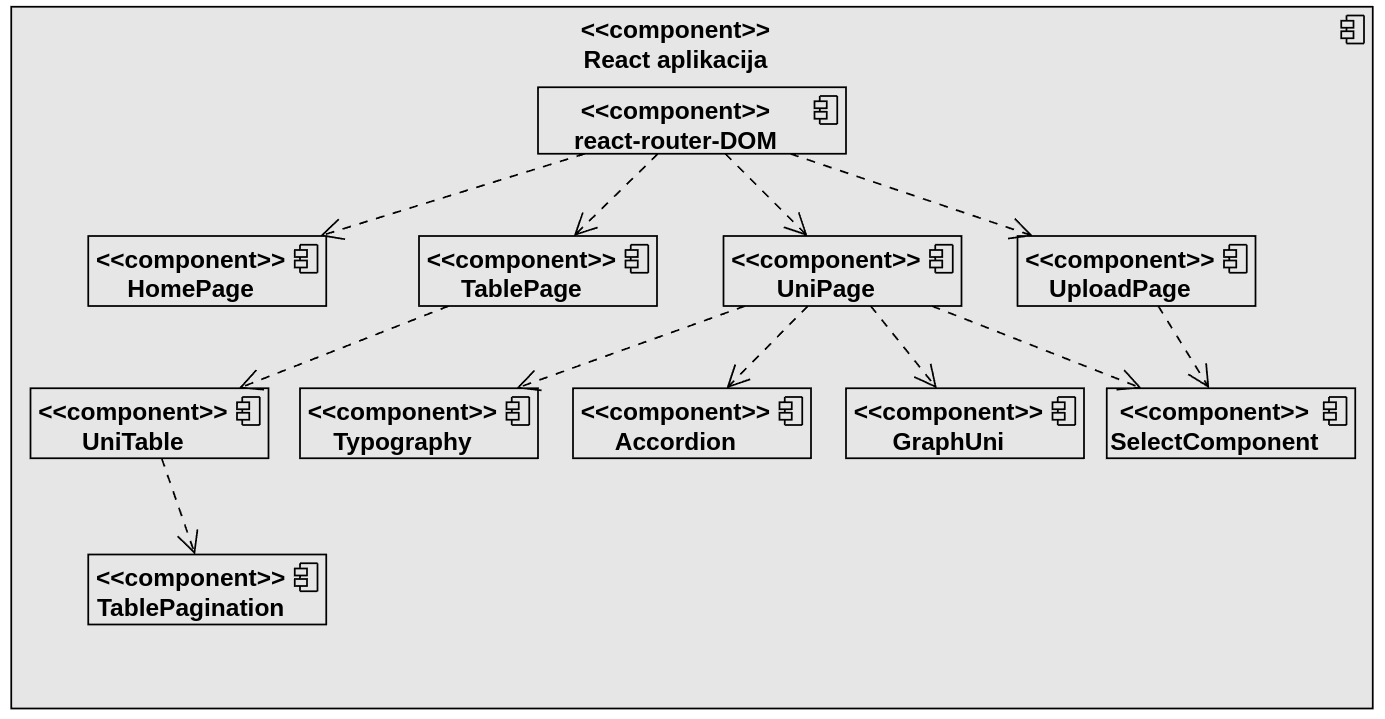
\includegraphics[scale=0.35]{reactkomponente.png} 
       \caption{Dijagram komponenti korisničkog sučelja}
       \label{fig:reactkomponente}
       \end{figure}
       \begin{table}[htb]
        \caption{Stranice iz dijagrama \ref{fig:reactkomponente} i njihov opis}
            \label{tbl:stranice}
            \centering
            \begin{tabular}{ll} \hline
            Naziv stranice & Opis\\ \hline
            \emph{HomePage} & početna stranica aplikacije\\
            \emph{TablePage} & tablični prikaz rang liste\\
            \emph{UniPage} & stranica s grafovima za praćenje napretka sveučilišta\\
            \emph{UploadPage} & stranica za objavu Shanghai Ranking podataka
            \end{tabular} 
            \end{table} 
            \FloatBarrier
Prema slici \ref{fig:reactkomponente} vidi se da je organizacija komponenti hijerarhijska jer svaka \\komponenta može gnijezditi proizvoljan broj drugih komponenti.
Dijagram \ref{fig:reactkomponente} sadrži navedene najbitnije komponente koje čine stranice ove aplikacije, osim njih \\postoje druge jednostavne komponente i HTML elementi 
koji čine konačnu stranicu. \\Komponente ove aplikacije su obične JavaScript funkcije koje vraćaju React elemente napisane JSX (\emph{JavaScript XML}) sintaksom koja 
omogućava kombiniranje HTML elemenata i JavaScript koda. Svaka komponenta može, kao i obična funkcija, primiti argumente koji se u Reactu zovu \emph{props}.
Drugi način oblikovanja React komponenti je pisanjem razreda, no verzijom Reacta 16.8 uvedena je funkcionalnost React \\\emph{useState hook} koja omogućava 
praćenje stanja komponente i u funkcijskim komponentama. Funkcijske komponente zahtijevaju pisanje manje programskog koda i \\jednostavnije su te se iz tog
razloga danas koriste više od razrednih komponenti. 
Praćenje stanja funkcijske komponente omogućava React \emph{useState hook} koji \\inicijalizacijom vraća polje veličine 2. Prvi element polja je varijabla u kojoj 
je pohranjena trenutna vrijednost stanja, a drugi element je referenca na funkciju s kojom se stanje može ažurirati. Svaka komponenta može imati 
proizvoljan broj stanja. Primjer inicijalizacije stanja koje pamti ocjenu uspješnosti rangiranja, inicijalna vrijednost je 0:
\begin{verbnobox}[\fontsize{10pt}{10pt}\selectfont]
const [index, setIndex] = React.useState(0)
\end{verbnobox}
Navedeno stanje koristi se unutar komponente \emph{TablePagination} i pomoću JSX sintakse vrijednost stanja može se prikazati na stranici koju korisnik vidi sljedećim \\programskim kodom:
\begin{verbnobox}[\fontsize{10pt}{10pt}\selectfont]
<div>
    Ocjena uspješnosti rangiranja: 
        {parseFloat((correct*100).toFixed(2)) || 0}
</div>
\end{verbnobox}
Svaki puta kada se vrijednost stanja \emph{correct} promijeni, ažurirat će se prvo Reactov virtualni DOM, a kasnije samo onaj dio koji se treba promijeniti u preglednikovom DOM-u.
Obavljanje radnji kada se vrijednost nekog stanja promijeni omogućava React \emph{hook useEffect} koji prima polje ovisnosti \engl{dependency array}. \emph{Hook useEffect}
pokreće se svaki put kad se komponenta prvi put iscrtava te kada vrijednosti stanja predanih u polju ovisnosti nemaju istu vrijednost koju su imali kod prošlog iscrtavanja.
Kombinacija funkcionalnosti \emph{useEffect} i \emph{useState} koristi se često u ovoj aplikaciji. Jedan primjer je dohvat podataka s poslužitelja 
kada se vrijednost nekog stanja ili više njih promijeni. Programski kod koji dohvaća podatke smješta se unutar \emph{useEffect} React \emph{hooka}.
Prilikom izrade stranice na kojoj je prikazana tablica rang liste \emph{useEffect} je korišten za dohvat podataka o uspješnosti procjene rangiranja:
\begin{verbnobox}[\fontsize{10pt}{10pt}\selectfont]
 React.useEffect(()=>{
    (async()=>{
        const request = await axios.get
            (`http://localhost:8080/difference
                /?year=${year}&category=${category}`,
        {
            headers: {'Content-Type':'application/json'},
            withCredentials: true
        });
        const response = request.data
        setCorrect(response.correct || 0)
      })()
},[year])
\end{verbnobox}
Prikazani \emph{useEffect} ima predano stanje \emph{year} u polju ovisnosti te svaki put kada korisnik putem komponente za odabir godine promijeni 
godinu za koju želi gledati rang listu, izvest će se funkcija unutar \emph{useEffect hooka} koja će dohvatiti ocjenu uspješnosti procjene rang liste te ažurirati stanje 
\emph{correct} čime će se automatski ažurirati i DOM te će korisnik imati prikaz uspješnosti rangiranja za odabranu godinu.
U prethodno prikazanom programskom kodu za stvaranje HTTP GET zahtjeva na poslužitelj korištena je biblioteka Axios.
\\\\Navigiranje aplikacijom omogućava vršna komponenta react-router-dom.
\\React-router-dom sastoji se od BrowserRouter, Routes, Route i Link komponenti. 
\\\\\textbf{BrowserRouter} komponenta brine se za sinkroniziranje URL-a i stranice koja se prikazuje korisniku. Ona je roditeljska komponenta koja umata sve ostale komponente za navigiranje aplikacijom.
\\\textbf{Routes} komponenta grupira pojedine Route komponente te ih veže za određenu putanju.
\\\textbf{Route} komponenta registrira pojedinu stranicu na određenu putanju iz URL-a.
\\\textbf{Link} komponenta služi za umatanje HTML elemenata ili vlastitih React komponenti tako da pritisak miša na tu komponentu korisnika odvede na novu stranicu.
\\\\Pritisak miša na recimo komponentu Link ne uzrokuje HTTP zahtjev za novom HTML stranicom jer su svi elementi stranica već preuzeti i nalaze se u korisnikovom \\pregledniku.
\\React-router-dom radi interno usmjeravanje i brine se da pritiskom na komponentu Link se promijeni URL preglednika i ažurira prikaz stranice koju korisnik vidi.
\\Primjer korištenja react-router-dom i registriranja stranice \emph{HomePage} na putanju \url{/}:
\begin{verbnobox}[\fontsize{10pt}{10pt}\selectfont]
<BrowserRouter>
    <Routes>
        <Route path="/" element = {<HomePage/>}></Route>
    </Routes>
</BrowserRouter>
\end{verbnobox}
Material UI biblioteka gotovih komponenti u ovoj aplikaciji korištena je za izradu dijelova pojedinih stranica. Primjer su komponente za odabir godine rangiranja
na stranici opisanoj u dijelu 5.2 te Accordion komponenta koja skriva odnosno prikazuje jedan od tri vrste grafa na stranici opisanoj u dijelu 5.3.
Material UI komponente koriste se kao obične React komponente kojima se mogu predati razni parametri za prilagođavanje vlastitim potrebama.
\\Graf komponenta ostvarena je React-chartjs-2 bibliotekom koja nudi brojne vrste grafova, a u ovoj aplikaciji korišten je linijski graf:
\begin{verbnobox}[\fontsize{10pt}{10pt}\selectfont]
<Line options={options} data={graphData}/>
\end{verbnobox}
Kako bi se graf ispravno nacrtao potrebno mu je predati vrijednosti oznaka na x i y osima.
\\\\Tailwind CSS radni okvir korišten je za izradu tablice rang liste prikazane na stranici 5.2. Tailwind CSS radi tako da skenira React datoteke 
te traži korištena imena CSS razreda te generira CSS datoteku sa željenim stilovima. Popis razreda koji se mogu koristiti nalazi se na službenoj
Tailwind CSS stranici.
\\ \subsection{Skupljač podataka za rangiranje}
U sljedećem dijelu opisane su tehnologije te detalji implementacije periodičkog \\skupljanja podataka za rangiranje.
\\\\\textbf{Node Cron}
\\ Node Cron je Node.js modul koji omogućava pozivanje JavaScript funkcija u željeno vrijeme. Node Cron modul se u ovoj 
aplikaciji koristi kako bi se svaka dva tjedna pokrenuo alat Puppeteer koji će prikupiti najnovije podatke za izračun ranga sveučilišta.
\\ \\ \textbf{Puppeteer}
\\ Puppeteer je Node.js biblioteka koja nudi bogati API pomoću kojeg se preglednici Chrome i Chromium mogu kontrolirati koristeći DevTools protokol.
DevTools protokol omogućuje alatima upravljanje preglednicima kao što su Chrome i Chromium na temelju uputa koje se predaju tim alatima.
Puppeteer je korišten za izradu \emph{web \\scrappera} (alat koji posjećuje web stranice i 
na njima obavlja neke radnje bez potrebe za intervencijom čovjeka) za baze InCites i WoS. Iako navedene baze nude API pomoću kojeg se svi
podatci potrebni za izračun rang liste mogu dohvatiti, on se plaća. Puppeteer alatu zadan je niz koraka koje treba obaviti na nekoj stranici (upisati tekst u neko polje, pritisnuti na gumb, otići na drugu stranicu)
kako bi se postigao željeni rezultat.
\\\\\textbf{Punjenje baze podataka i korištenje alata Puppeteer}
\\Prilikom prvog pokretanja poslužiteljske aplikacije potrebno je stvoriti tablice u bazi podataka i napuniti ih vrijednostima indikatora od prijašnjih godina.
Vrijednosti svih indikatora, osim indikatora \emph{Award}, mogu se dobiti s InCites stranice. Vrijednosti \\indikatora \emph{Award} teže je automatski prikupljati 
s web stranica zbog potrebne analize institucija s kojima je dobitnik nagrade u vrijeme dobitka bio povezan. Iz tog razloga ti podatci 
su ručno prikupljeni te kasnije uneseni u bazu podataka. 
\\Dio programskog koda koji inicijalno puni bazu podataka nalazi se prema slici \ref{fig:expressdijagramkomponenti} u komponenti podatkovni modeli. Lakše prikupljanje podataka sa stranice InCites omogućava izrada predložaka za pretragu koji se mogu pohraniti 
na korisničkom profilu u odjeljku \emph{Dashboard}. Ukupno su pohranjena 4 predloška. Za svaku od kategorija CSE i EEE pohranjen je predložak 
za dohvat indikatora Q1, CNCI, IC te još jedan predložak za indikator \emph{Top}. U svakom predlošku unaprijed su odabrani filteri kao što su područje istraživanja,
vrsta organizacije, vrsta dokumenta i vremenski period. Indikator \emph{Top} ima vlastiti predložak jer zahtjeva unos filtera prema časopisima za područje EEE te 
prema konferencijama za područje CSE. 
\begin{figure}[htb]
    \hspace*{-2cm} 
       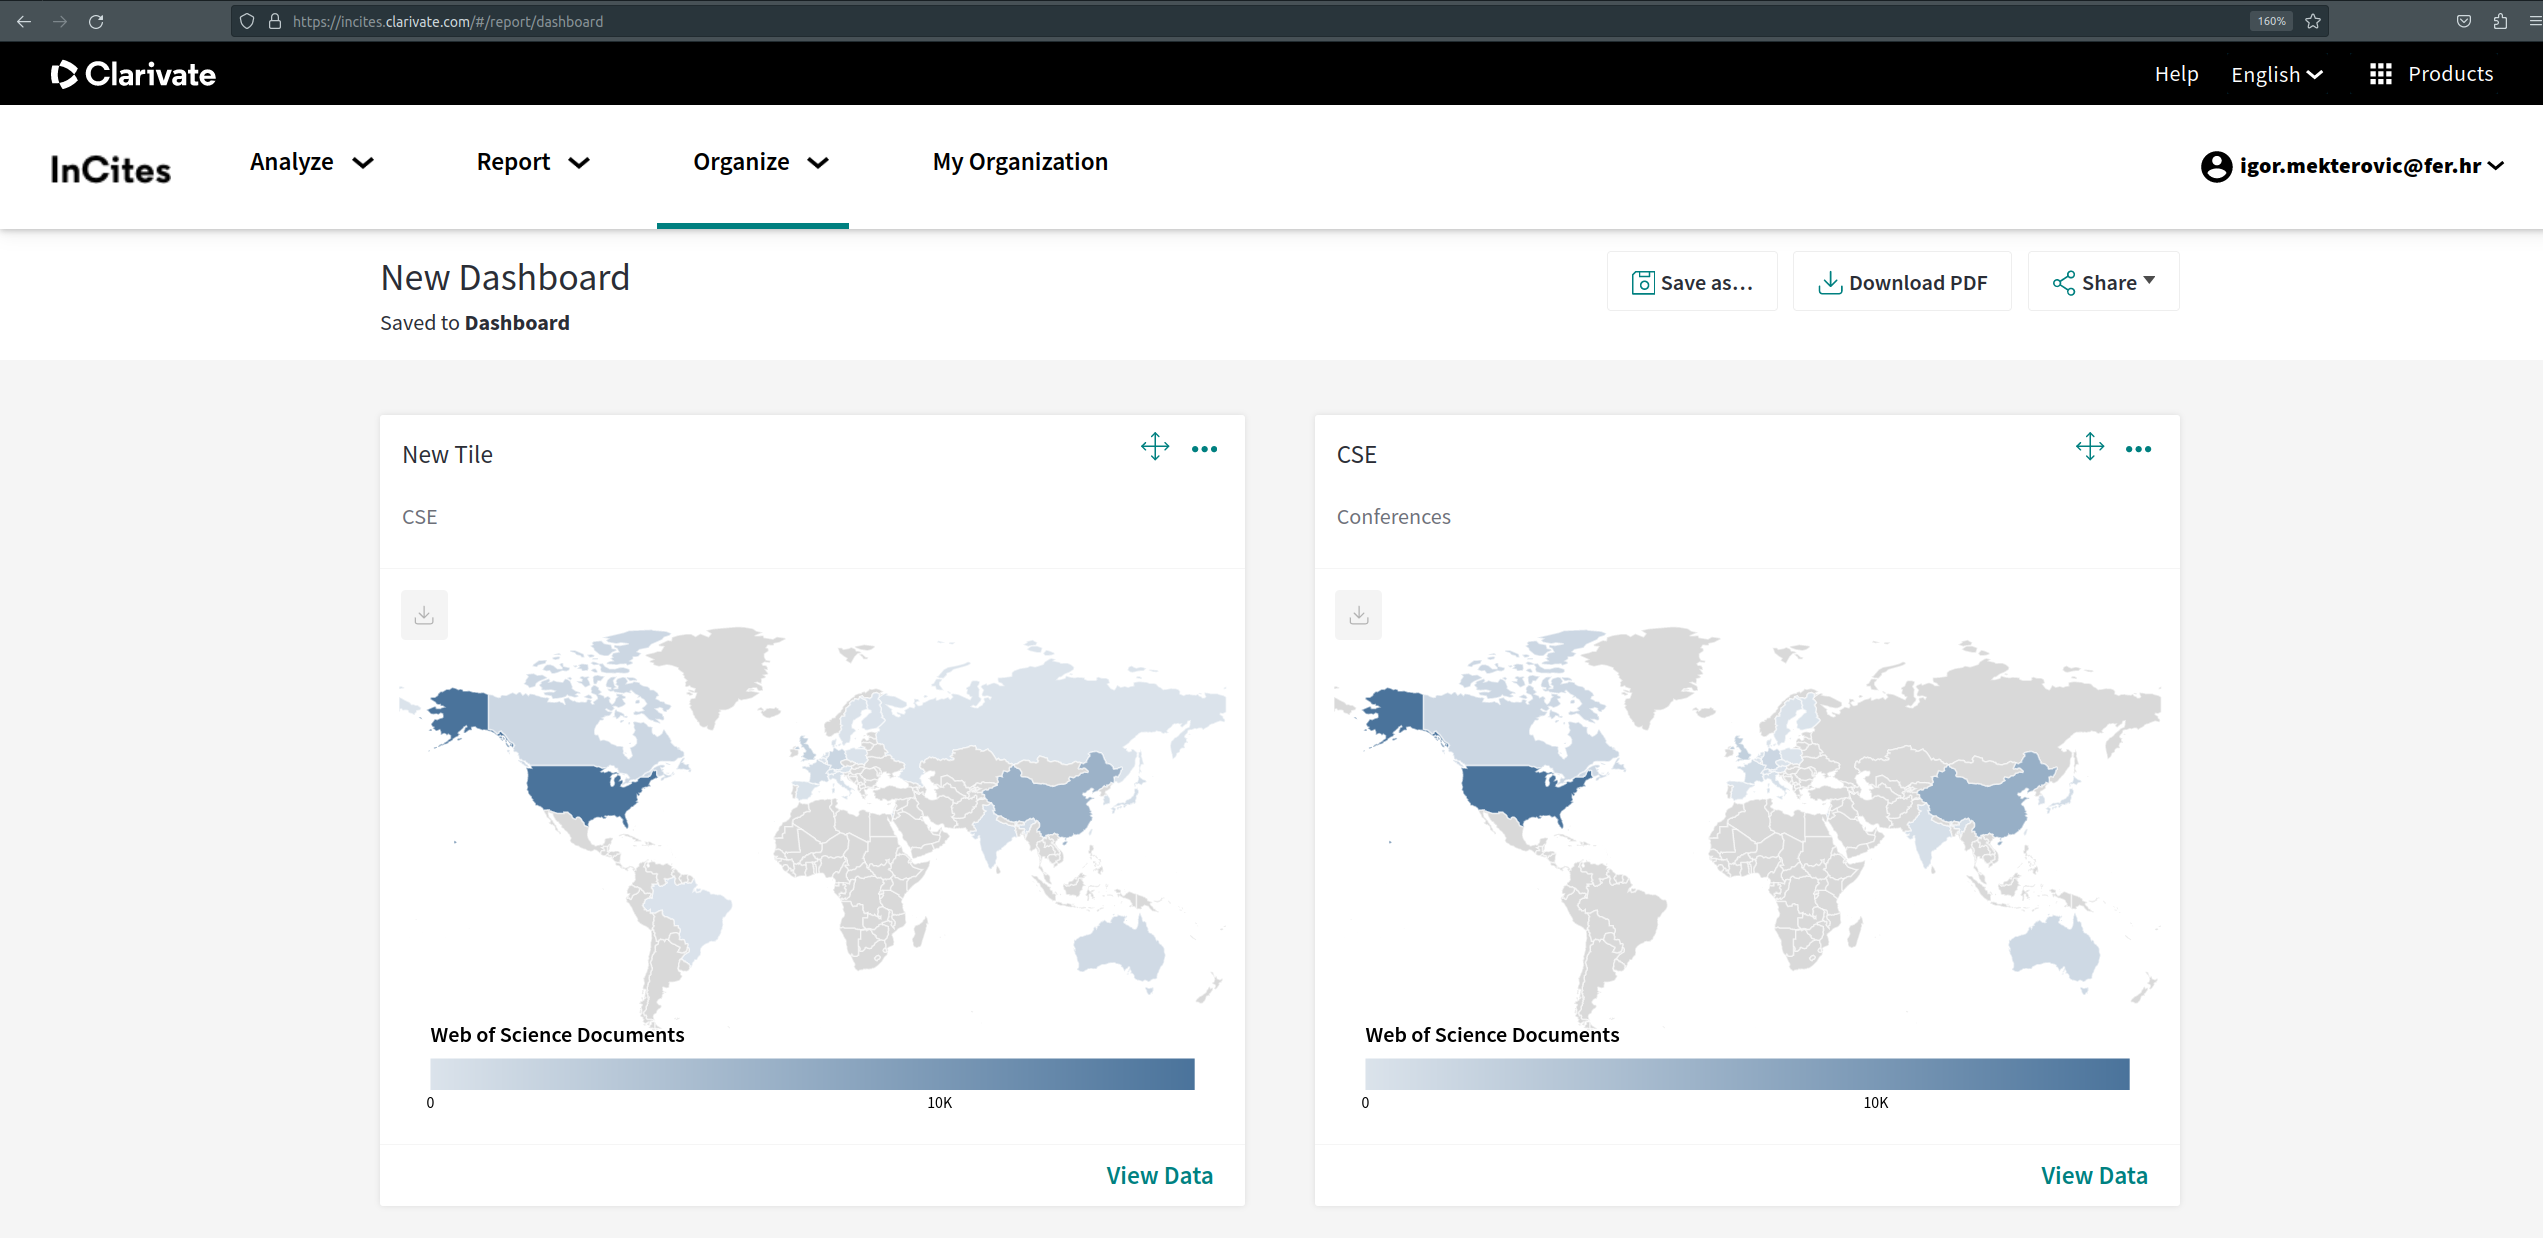
\includegraphics[scale=0.21]{dashboard.png} 
       \caption{Stranica \emph{Dashboard} na InCites aplikaciji}
       \label{fig:dashboard}
       \end{figure} 
\begin{figure}[htb]
        \hspace*{-2cm} 
           
\includegraphics[scale=0.21]{predlozak.png} 
           \caption{Primjer izgleda predloška za dohvat vrijednosti indikatora}
           \label{fig:predlozak}
           \end{figure}  
           \FloatBarrier      
\begin{figure}[htb]
    \centering
       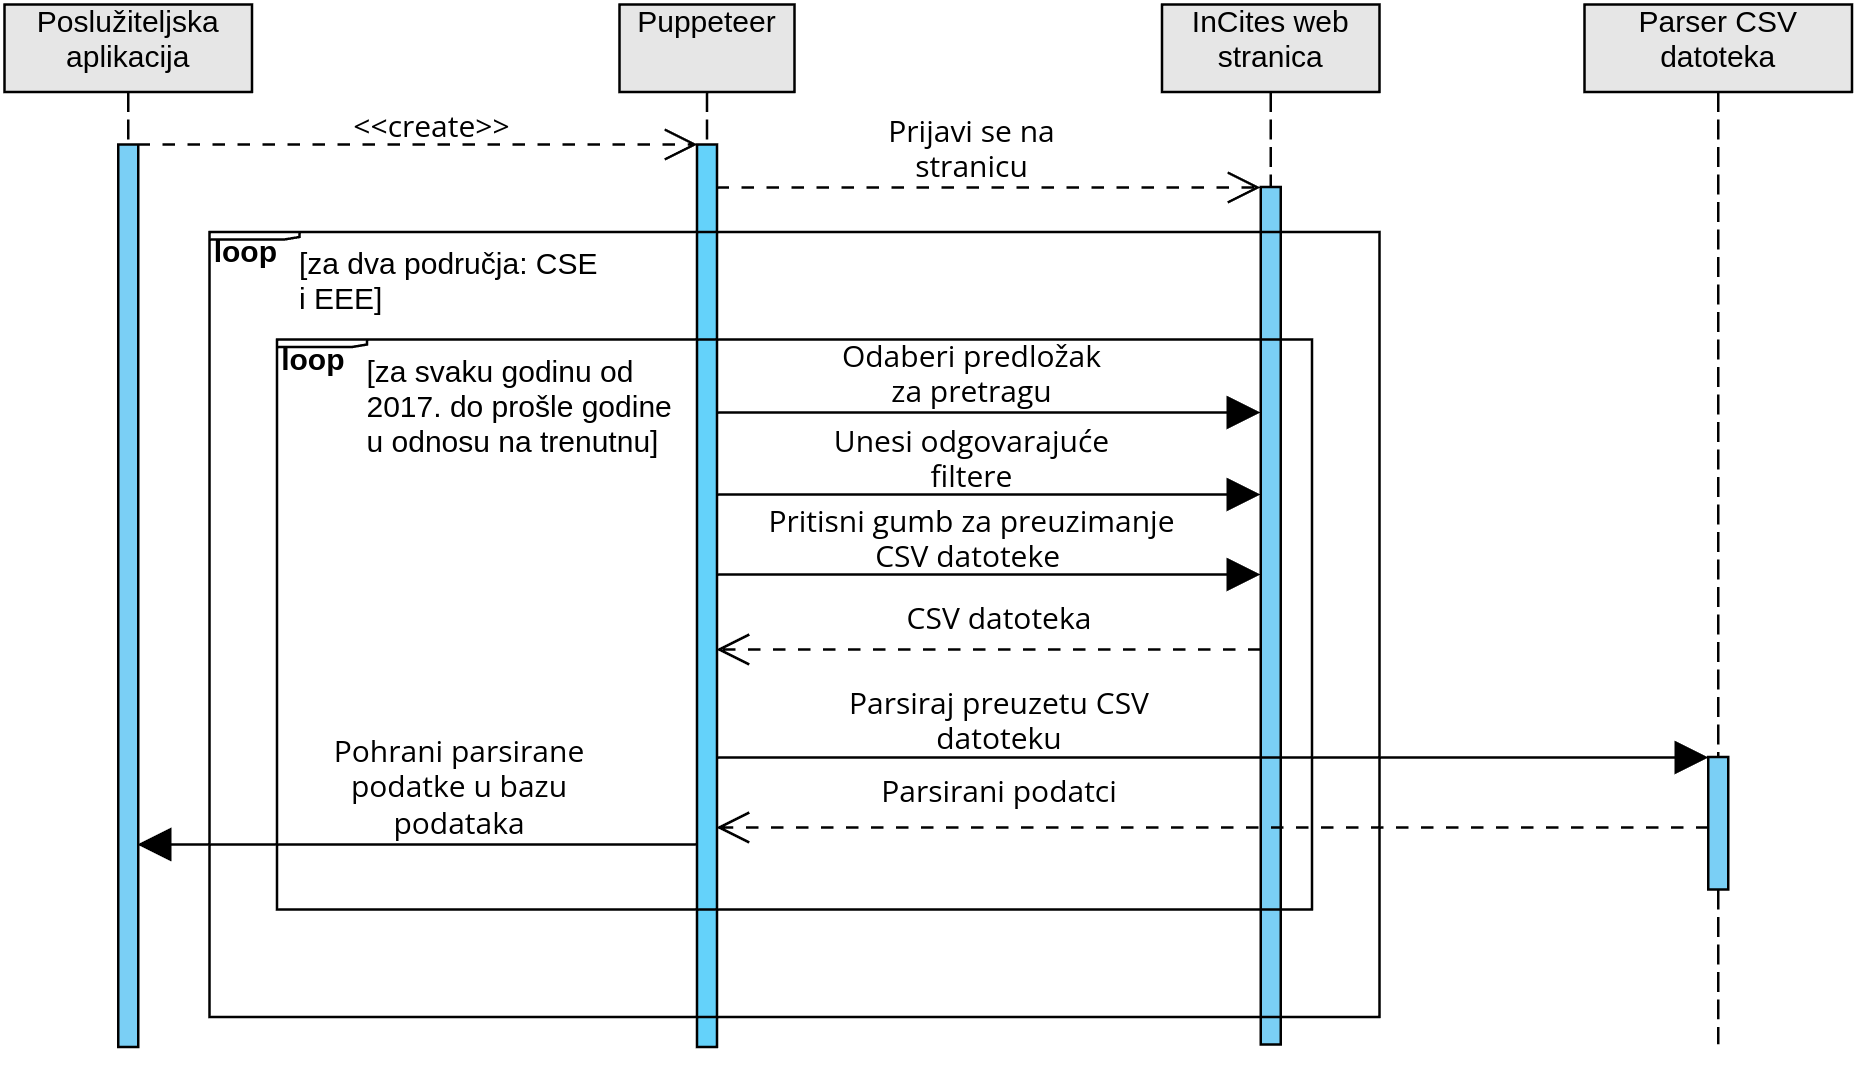
\includegraphics[scale=0.22]{sekvencijski.png} 
       \caption{Sekvencijski dijagram inicijalnog punjenja baze podataka}
       \label{fig:sekvencijski}
       \end{figure}
       \FloatBarrier
Prema sekvencijskom dijagramu sa slike \ref{fig:sekvencijski} funkcija koja inicijalno puni bazu podataka mora za svako područje i
godinu od 2017. do prošle u odnosu na trenutnu prikupiti sve vrijednosti indikatora potrebnih za izračun rang liste.  
\\Programski kod funkcije koja inicijalno puni bazu podataka:        
\begin{verbnobox}[\fontsize{10pt}{10pt}\selectfont]
(async()=>{
    let number = 0;
    try{
        let rows = (await pool.query(`select count (*) 
                        from ranking`, [])).rows
        number = rows[0].count
    } catch(exception){
        console.log('Greška prilikom dohvata podataka iz tablice ranking.')
    }
    if(number == 0){
        await createTables();
        await seedAward("EEE")
        await seedAward("CSE")
        await seedRealRanking();
            
        dataSelector1 = `[aria-label=`View more 
                                data for EEE1`]`
        dataSelector2 = `[aria-label=`View more 
                                data for EEE2`]`
        await seedIndicators("EEE", dataSelector1, 
                                dataSelector2, 2017, 
                                new Date().getFullYear()-1, 
                                6, 2, 'ranking')
    
        dataSelector1 = `[aria-label=`View more
                             data for CSE1`]`
        dataSelector1 = `[aria-label=`View more
                             data for CSE2`]`
        await seedIndicators("CSE", dataSelector1, 
                                dataSelector2, 2017, 
                                new Date().getFullYear()-1,
                                6, 2, 'ranking')
    }
})()
\end{verbnobox}  
Funkcija provjerava je li relacija \emph{ranking} već popunjena podatcima te nastavlja s \\izvršavanjem samo ako je prazna. 
Za oba područja CSE i EEE puni bazu podataka vrijednostima indikatora \emph{Award} te zatim priprema CSS selektore koji će omogućiti alatu 
Puppeteer pritisak na odgovarajući predložak. Funkcija poziva drugu \\funkciju \emph{seedIndicators} koja kao argumente redom prima:

    a) područje istraživanja
    
    b) CSS selektor prvog predloška 

    c) CSS selektor drugog predloška
    
    d) donju i gornju granicu godina za koje će se prikupiti podatci
    
    e) dva broja pomoću kojih se izračuna donja i gornja granica vremenskog perioda tijekom kojeg se uzimaju podatci za izračun rang liste određene godine
        (prema \\Shanghai Ranking algoritmu taj period je 5 godina, a postupak izračuna granica objašnjen je u dijelu 2.)
      
    f) ime relacije u koju će se unijeti dohvaćeni podatci.
\\\\Inicijalizacija alata Puppeteer radi se sljedećim programskim kodom:
\begin{verbnobox}[\fontsize{10pt}{10pt}\selectfont] 
const browser = await puppeteer.launch({
    executablePath: '/usr/bin/google-chrome',
    headless: true,
    args: [
        "--disable-gpu",
        "--disable-dev-shm-usage",
        "--disable-setuid-sandbox",
        "--no-sandbox",
        ]
});
\end{verbnobox}  
Kako bi alat ispravno radio unutar Docker kontejnera mora se postaviti parametar \\\emph{executablePath} koji predstavlja putanju 
do preglednika kojeg Puppeteer koristi, isključiti grafičko sučelje preglednika postavljanjem parametra \emph{headless} na \emph{true} te predati 
polje argumenata koji omogućavaju dodatnu konfiguraciju, a preporučeni su u dokumentaciji alata za upotrebu unutar kontejnera.
Nakon što je alat instanciran putem dobivene reference može se navigirati na željenu stranicu koristeći funkciju \emph{goto(\url{"url/stranice"})}.
\\Jednom kad je stranica učitana moguće je obavljati razne akcije na stranici kao što su:

    a) pritisak na gumb s funkcijom \emph{click("CSS selektor")}

    b) upisati tekst u polje za unos teksta s funkcijom \emph{type("CSS selektor", "tekst za unos")}

    c) pričekati obavljanje daljnjih akcija dok se željeni HTML element nije učitao koristeći funkciju \emph{waitForSelector("CSS selektor")}.
\\Kombinacijom navedenih funkcija moguće je preuzeti podatke u obliku CSV datoteke koji su nakon parsiranja spremni za unos u bazu podataka.
Programski kod navigiranja stranicom koristeći alat Puppeteer te parsiranje preuzetih CSV datoteka nalazi se prema 
dijagramu \ref{fig:expressdijagramkomponenti} u sklopu pomoćnih servisa.
\\\\Procjena vrijednosti indikatora trenutne godine te periodičko punjenje baze podataka s \\vrijednostima indikatora kako bi se mogao pratiti napredak 
sveučilišta kroz tekuću godinu ostvareno je pozivanjem funkcije \emph{seedIndicators} svaka dva tjedna. Pozivanje funkcije svaka dva tjedna 
ostvareno je Node.js modulom Node cron. 
\\\\Primjer korištenja modula Node cron:
\begin{verbnobox}[\fontsize{10pt}{10pt}\selectfont] 
    const job = new cron.CronJob(`0 0 */14 * *`, 
                            async function() {
                await scheduledFunction();}, 
                null, false, 'UTC');
    job.start();
\end{verbnobox}  
Node cron modul nalaže da se inicijalizira jedan \emph{posao}. Za inicijaliziranje posla potrebno je predati sljedeće argumente:

    a) \emph{string} koji označava koliko često i kada će se funkcija predana u drugom argumentu pozivati (u ovom primjeru to je svakih 14 dana)

    b) funkciju koja će se pozvati kad za to dođe vrijeme

    c) funkcija koja će se pozvati nakon što se posao zadan drugim argumentom obavio 

    d) \emph{boolean} parametar koji označava hoće li se posao pokrenuti odmah prilikom izlaska iz konstruktora

    e) \emph{string} koji označava vremensku zonu
\\Funkcija \emph{scheduledFunction} poziva funkcije \emph{seedAward} i \emph{seedIndicators}. Argumenti funkcije \emph{seedIndicators}  
koji označavaju donju i gornju granicu godina za koje će se prikupiti podatci su isti te imaju vrijednost trenutne godine.
\\ \subsection{Poslužitelj web-aplikacije}
U sljedećem dijelu opisane su tehnologije te detalji implementacije poslužitelja web-aplikacije.
\\\\
\textbf{Node.js} 
\\ Node.js je JavaScript pokretačko okruženje \engl{runtime environment} namijenjeno izvođenju na poslužiteljskoj strani. Pokreće se na V8 JavaScript \emph{engineu}
te omogućuje izvršavanje JavaScript koda izvan preglednika. Koristi asinkronu arhitekturu zasnovanu na događajima \engl{asynchronous event-driven architecture}
te nudi mogućnost izrade skalabilnih aplikacija. 
\\\textbf{Express.js}
\\ Express.js je radni okvir \engl{framework} Node.js-a te omogućava izradu RESTful API-ja \engl{Application Programming Interface}. Express.js nudi
lagano upravljanje HTTP zahtjevima i izradu krajnjih točaka \engl{endpoint} s kojima će React aplikacija komunicirati.
\\ \\ \textbf{Node-postgres} 
\\ Kako bi poslužitelj mogao komunicirati s bazom podataka koristi se Node-postgres. To je skup Node.js modula koji nude 
sučelje prema bazi podataka. Pomoću ovog proširenja s poslužitelja se mogu raditi sve uobičajene radnje s bazom podataka (stvaranje novih tablica, 
unos podataka u tablice, dohvaćanje podataka iz tablica, brisanje podataka iz tablica i razne druge radnje).
Node-postgres stvara bazen otvorenih veza \engl{connection pool}. Koristeći \emph{connection pool} jednom otvorena veza s bazom podataka može se koristiti više puta te se ne mora 
stvarati nova veza s bazom podataka za svaki novi korisnički upit čime se štedi vrijeme i smanjuje mogućnost pogreške. Novostvoreni \emph{connection pool} inicijalno 
je prazan te se nove veze dodaju lijeno, po potrebi.
\begin{figure}[htb]
    \hspace*{-2cm} 
       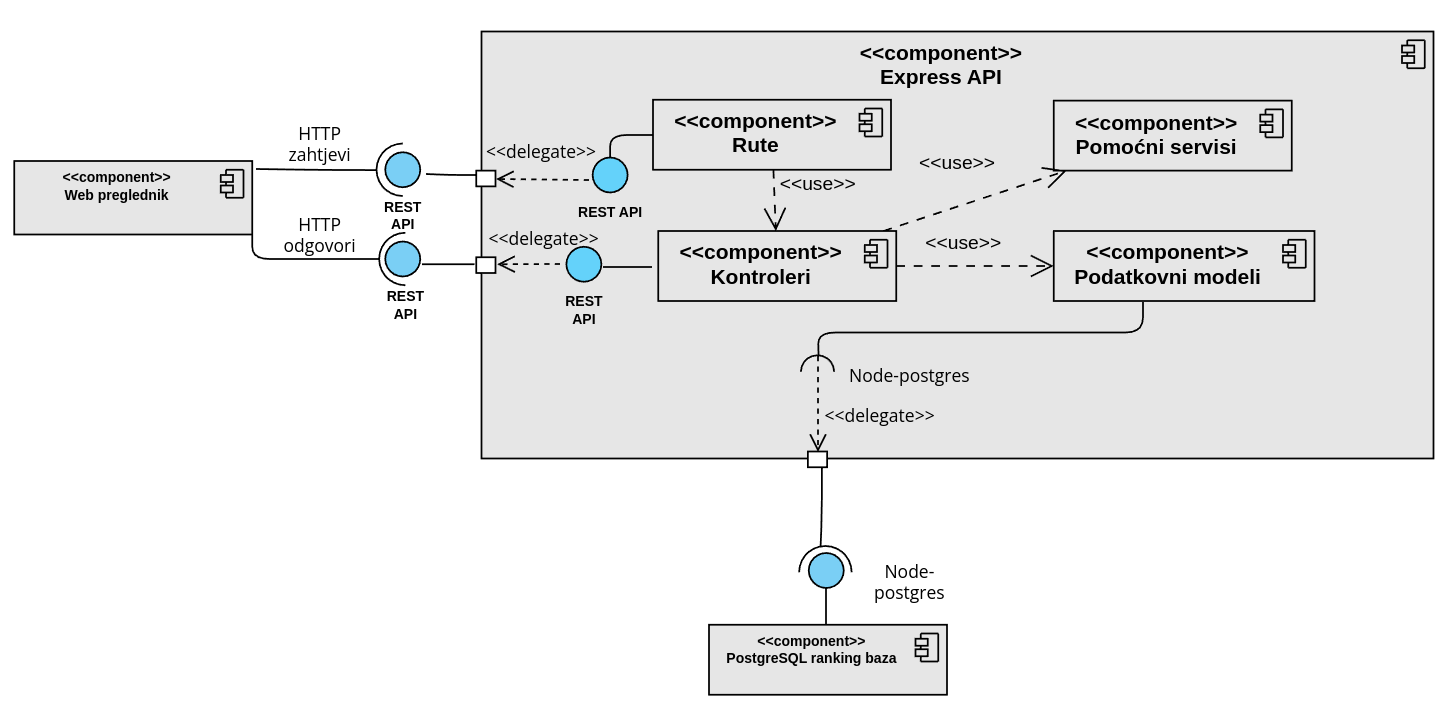
\includegraphics[scale=0.36]{expressdijagramkomponenti.png} 
       \caption{Dijagram komponenti Express API-ja, korisničkog preglednika te baze podataka}
       \label{fig:expressdijagramkomponenti}
       \end{figure}      
\\\\Poslužiteljska strana nudi React korisničkom sučelju RESTful API, a komunikacija se odvija putem HTTP protokola. Podatke za ažuriranje sadržaja stranice 
React \\korisničko sučelje dohvaća s poslužitelja koristeći RESTful API kako je prikazano na slici \ref{fig:expressdijagramkomponenti}.
\\\\\\\textbf{Krajnje točke i kontroleri}
\\Krajnje točke \engl{endpoint} RESTful API-ja ostvarene su upotrebom usmjerivača \engl{router} i kontrolera u sklopu Express radnog okvira. 
Prije nego što Express aplikacija može primati HTTP zahtjeve, potrebno je registrirati rute i povezati ih s odgovarajućim \emph{routerima}.
Primjer registriranja rute \url{/rankingReal} i povezivanja na \emph{router} \emph{getRealRanking} gdje varijabla \emph{app} predstavlja instancu Express aplikacije:
\begin{verbnobox}[\fontsize{10pt}{10pt}\selectfont] 
app.use('/rankingReal', require('./routes/getRealRanking'))
\end{verbnobox}  
Dolaskom HTTP zahtjeva na poslužitelj Express aplikacija provjerava postoji li ruta koja se podudara s registriranim rutama te ako postoji 
zahtjev preusmjerava na definirani \emph{router}.
\\\emph{Routeri} su dio Express radnog okvira koji omogućavaju definiranje raznih \emph{middleware} funkcija koje će se izvršavati 
na nekoj ruti.
\emph{Middleware} funkcije se izvršavaju između prijema HTTP zahtjeva i slanja HTTP odgovora. Primjer definiranja \emph{middleware}
\\funkcija za HTTP GET zahtjev na ruti \url{/rankingReal}:
\begin{verbnobox}[\fontsize{10pt}{10pt}\selectfont]  
const express = require('express');
const router = express.Router();
const getRealRanking = require(
            '../controllers/getRealRankingUni')
router.get('/', 
    getRealRanking.getRealRankingForYearUniCategory)
module.exports = router
\end{verbnobox}  
Iz priloženog programskog koda vidi se da je \emph{middleware} funkcija definirana u kontroleru \emph{getRealRankingUni}:
\begin{verbnobox}[\fontsize{10pt}{10pt}\selectfont] 
const getRealRankingForYearUniCategory = async (req, res)=>{
    const{ year, category, uni } = req.query
    let results = await getRealRanking(uni, year, category)
    if(results.length > 0){
        results[0].total = results[0].q1+results[0].cnci+
        results[0].ic*0.2+results[0].top+results[0].award
    }
    return res.json(results[0])
}
\end{verbnobox} 
Parametri iz URL-a kod HTTP GET zahtjeva dostupni su unutar objekta \emph{req.query}, a JSON tijelo poruke koje se šalje kod POST zahtjeva u objektu \emph{req.body}.
\emph{Middleware} funkcije u kontrolerima obavljaju neku poslovnu logiku, komuniciraju s bazom podataka te vraćaju rezultat HTTP zahtjeva u JSON obliku.
\begin{table}[htb]
    \caption{Krajnje točke poslužitelja}
        \label{tbl:endpoints}
        \centering
        \begin{tabular}{llll} \hline
        Redni broj & Ruta & Vrsta zahtjeva & Dodatni parametri\\ \hline
        1. & \url{/rankingsYear} & GET & \emph{page, limit, search, orderid, orderkey} \\
        &&&\emph{year, category}
        \\2. & \url{/rankingUni} & GET & \emph{year, category, uni}
        \\3. & \url{/uniCurrentYear} & GET & \emph{uni, category}
        \\4. & \url{/rankingReal} & GET & \emph{year, category, uni}
        \\5. & \url{/difference} & GET & \emph{ year, category}
        \\6. & \url{/upload} & POST & \emph{-}
        \end{tabular}
        \end{table} 
        \FloatBarrier
Krajnja točka rednog broja 1 iz tablice \ref{tbl:endpoints} koristi se za ostvarenje paginacije tablice rang liste za neku godinu u nekom području.
Pomak od prvog zapisa rang liste računa se pomoću parametara \emph{page}, a broj zapisa koje treba vratiti pomoću parametra \emph{limit}.
Sortiranje rang liste prema željenoj vrijednosti indikatora omogućeno je parametrima \emph{orderkey} i \emph{orderid}.
\emph{Orderkey} je \emph{boolean} vrijednost koja označava silazno, odnosno uzlazno sortiranje, a \emph{orderid} je oznaka indikatora
prema kojem se rang lista sortira. Pretraga sveučilišta po imenu omogućena je parametrom \emph{search} koji predstavlja \\podniz koji je korisnik unio 
kroz grafičko sučelje.
\\

Krajnje točke rednog broja 2, 3, 4 iz tablice \ref{tbl:endpoints} služe za dohvat podataka s kojima se crtaju grafovi na stranici objašnjenoj u 
dijelu 5.3. Sve tri krajnje točke primaju parametre \emph{year, category, uni} osim one rednog broja 3 jer se za parametar \emph{year} podrazumijeva 
da je riječ o trenutnoj godini.
\\

Krajnja točka rednog broja 5 iz tablice \ref{tbl:endpoints} služi za dohvat uspješnosti procjene \\rang liste neke godine u određenom području.
\\

Krajnja točka rednog broja 6 iz tablice \ref{tbl:endpoints} služi za postavljanje .xlsx datoteka u kojoj su zapisani stvarni Shanghai Ranking podatci 
koji se kasnije koriste za usporedbu s procijenjenim vrijednostima indikatora.
\subsection{Docker}
Kako bi se ova aplikaciju mogla lako postaviti \engl{deploy} na neki poslužitelj te tako omogućiti svim korisnicima pristup aplikaciji,
koristi se platforma Docker. Docker je platforma otvorenog koda koja se koristi za razvoj, isporuku i pokretanje aplikacija.
Docker se u ovom završnom radu koristi za pakiranje dijelova aplikacije u odvojene dijelove koji se zovu kontejneri \engl{containers}.
Kontejneri su zapravo Docker slike \engl{images} u izvođenju. Docker slika je lagana \engl{lightweight} komponenta koja sadrži sve što je aplikaciji 
potrebno za izvođenje (izvorni kod, pokretačko okruženje \engl{runtime}, razne alate i biblioteke). Način stvaranja docker slike se definira 
datotekom Dockerfile. Jednom kad je stvorena Docker slika, može se pokrenuti. Time se dobije kontejner koji se izvršava na Docker Engineu. 
Velika prednost Dockera je ta što je podržan na puno operacijskih sustava (Windows, Linux, MacOS i ostali) te se uz pomoć samo jedne naredbe i datoteke Dockerfile
dobije pokrenuta i funkcionalna aplikacija. Aplikacije koje se pokreću kao kontejneri rade na jednak način na svim operacijskim sustavima zbog ugrađene virtualizacije.
Docker virtualizira operacijski sustav, a ne sklopovlje. Ovo je velika prednost u odnosu na virtualizaciju koju rade virtualni strojevi. 
Virtualni strojevi emuliraju sklopovlje i upravljanjem pomoću hipervizora omogućuju da se na istom sklopovlju izvršava više operacijskih sustava. 
Docker kontejneri dijele isti operacijski sustav te svaki predstavlja poseban proces, zauzimaju manje 
resursa, lakši su i brži te za ostvarenje funkcionalnosti koriste jezgru operacijskog sustava Linux.

\begin{figure}[htb]
    \hspace*{-1cm}
    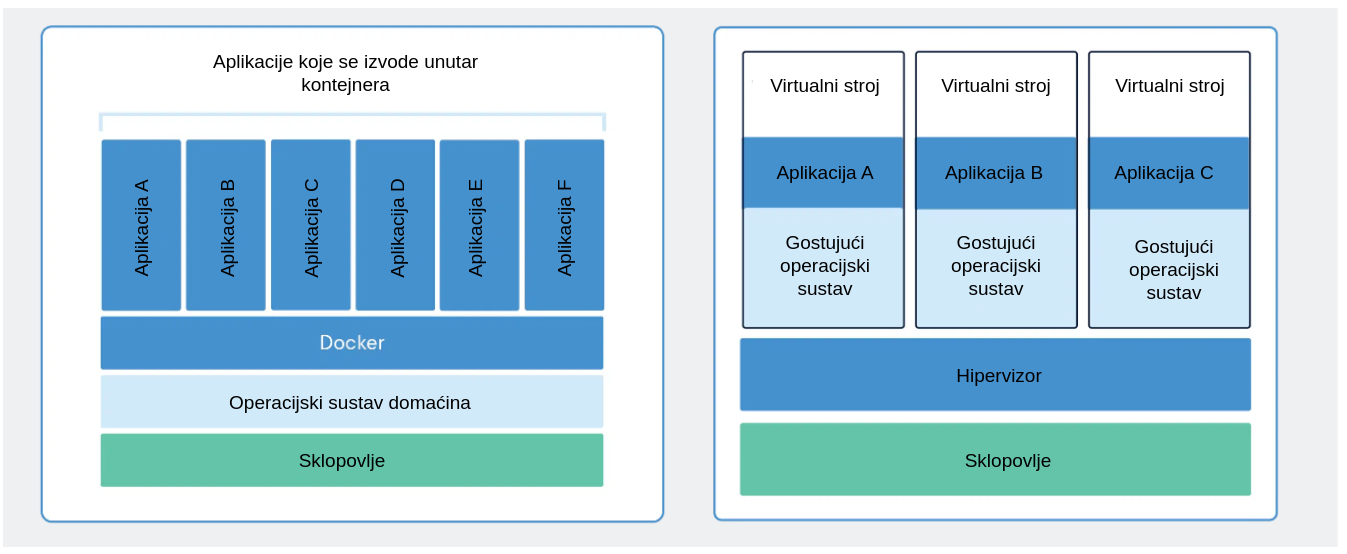
\includegraphics[scale=0.36]{slika2.png}
    \caption{Usporedba virtualnih strojeva (desno) i Docker načina virtualizacije (lijevo)}
    \label{fig:docker}
    \end{figure}

U slučaju ove aplikacije postoje 3 Docker slike koje će postati Docker kontejneri prilikom izvođenja. Jedna slika je za bazu podataka,
druga za poslužitelj, a treća za korisničko sučelje. Jednom kada je napisan Dockerfile za sve navedene dijelove aplikacije, dijelovi se povezuju  
datotekom docker-compose. U toj datoteci stoje upute od kojih se sve kontejnera aplikacija sastoji, kako kontejneri međusobno surađuju te kako se pokreću. Zahvaljujući 
ovoj datoteci, umjesto da se svaki kontejner posebno inicijalizira i pokrene, s jednom naredbom se pokrene cijela aplikacija.
Po jedna Dockerfile datoteka nalazi se u korijenskom direktoriju poslužitelja i 
React aplikacije. Unutar Dockerfile datoteke potrebno je navesti sve korake koji se moraju obaviti kako bi se kontejner uspješno pokrenuo te konfigurirati
određene parametre.
\\Za React aplikaciju i Express API potrebno je konfigurirati korijenski direktorij unutar kojeg će kontejner raditi, instalirati sve dodane module naredbom \emph{npm install}, 
podesiti pristup \engl{port} kojeg će aplikacija koristiti, kopirati izvorni kod aplikacije u radni direktorij kontejnera te napisati naredbu kojom se 
aplikacija pokreće. \\Prethodnim razvijanjem aplikacije svi potrebni moduli već su instalirani te kako bi se\\izbjeglo njihovo dupliciranje u direktoriju kontejnera potrebno je dodati 
.dockerignore datoteku unutar koje se navodi imena direktorija i datoteka koje se ne kopiraju u korijenski direktorij kontejnera.
Dockerfile Express API-ja razlikuje se malo od onog za React aplikaciju jer je potrebno instalirati odgovarajući preglednik kojeg alat \\Puppeteer može koristiti.
Alat Puppeteer bi sam instalirao preglednik Chromium no on zahtjeva dodatna podešavanja kako bi radio, iz tog razloga instaliran je preglednik Google Chrome koji 
dolazi automatski podešen.
\\Kada su napisane datoteke Dockerfile potrebno ih je povezati s datotekom \\docker-compose. Datoteka docker-compose sadrži putanje do svih Dockerfile datoteka koje 
čine aplikaciju, imena koja će se dodijeliti pojedinim kontejnerima, \\vrijednosti varijabla okoline, mapiranje pristupa kontejnera na pristupe računala na \\kojem se izvršava kontejner te
upute za stvaranje kontejnera unutar kojeg se pokreće \\PostgreSQL baza podataka.
\begin{figure}[htb]
    \hspace*{-2cm}
       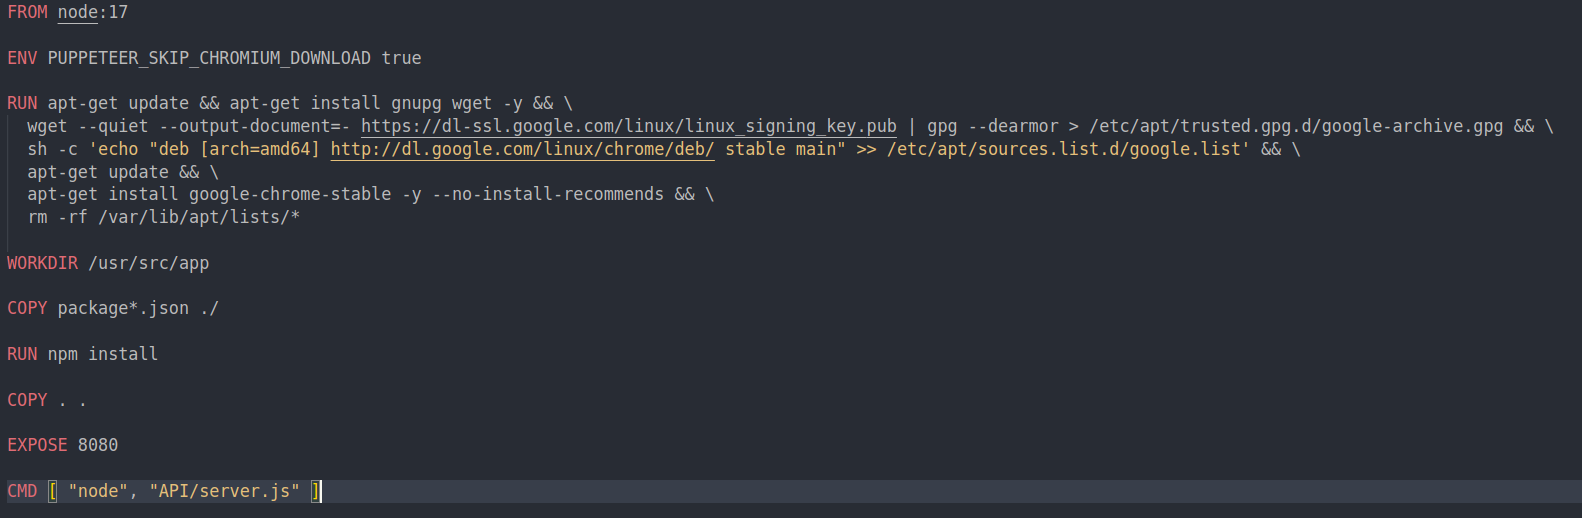
\includegraphics[scale=0.33]{dockerfile.png} 
       \caption{Dockerfile datoteka za Express API}
       \label{fig:docker1}
       \end{figure}
\begin{figure}[htb]
        \centering
           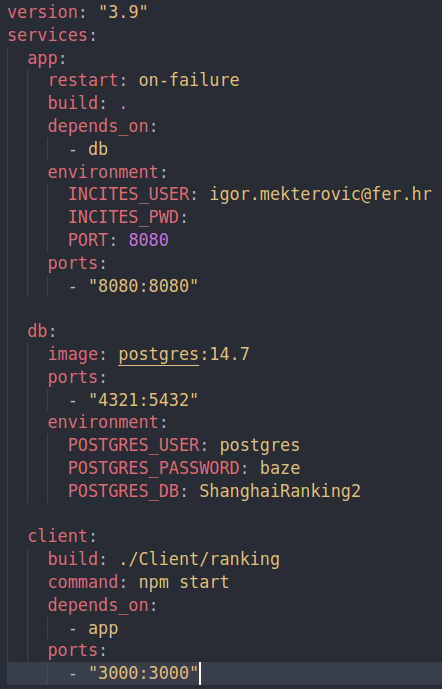
\includegraphics[scale=0.3]{docker2.png} 
           \caption{Docker-compose datoteka}
           \label{fig:docker2}
           \end{figure}       
           
Pokretanje baze podataka, Express API-ja te React aplikacije sada je moguće \\naredbom: \emph{docker-compose up}. Kada se Express API prvi put pokrene, krenut će se 
puniti baza podataka tako da sve vrijednosti indikatora neće biti dostupne odmah već nakon nešto više od 15 minuta.
\begin{figure}[htb]
    \centering
    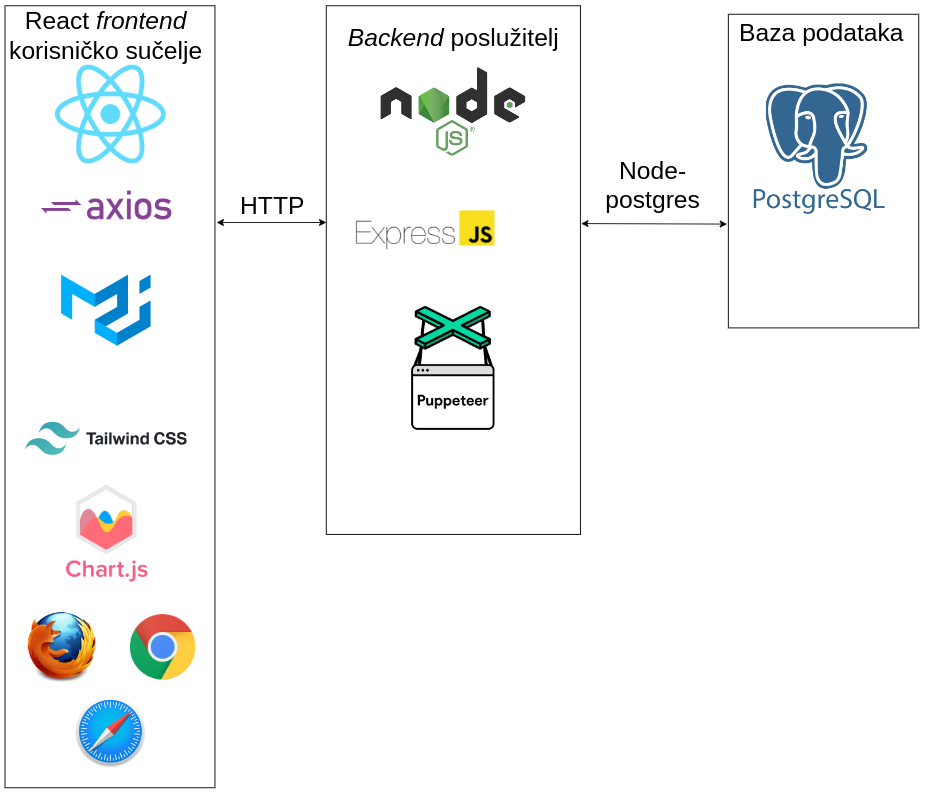
\includegraphics[scale=0.3]{tehnologije.png}
    \caption{Prikaz raspodjele korištenih tehnologija po arhitekturnim slojevima}
    \label{fig:arhitektura}
    \end{figure}
           \chapter{Podatkovni model}
           Ova aplikacija temelji se na tri relacije u PostgreSQL bazi podataka. Nazivi relacija su: \emph{award}, \emph{ranking} i \emph{rankingreal}.
           \section{Relacija \emph{award}}
           \begin{table}[htb]
               \caption{Atributi relacije \emph{award}}
                   \label{tbl:award}
                   \centering
                   \begin{tabular}{llr} \hline
                   Naziv atributa & Tip podatka & Opis\\ \hline
                   \emph{id} &  \emph{integer} & jedinstveni identifikator zapisa i primarni ključ relacije\\
                   \emph{uni} &  \emph{text} & naziv sveučilišta\\
                   \emph{year} &  \emph{integer} & godina osvajanja nagrade\\
                   \emph{share} &  \emph{double precision} & udio bodova sveučilišta\\
                   \emph{category} &  \emph{text} & naziv područja za koje je nagrada osvojena\\
                   \end{tabular}
                   \end{table}    
                   \FloatBarrier 
           Relacija \emph{award} sadrži podatke o osvojenim nagradama sveučilišta. Svaki zapis sadrži atribut \emph{share} koji označava 
           koliko bodova na rang listi će sveučilište dobiti u ovisnosti o tome s koliko institucija je osvajač nagrade za vrijeme dobitka nagrade
           surađivao. Postupak izračuna udjela opisan je u odjeljku \ref{indikatori}, a predstavlja recipročan broj broja institucija s kojima je osvajač 
           nagrade surađivao. Svaki zapis također ima i atribut \emph{category} koji označava područje u kojem je nagrada osvojena te može biti CSE ili EEE.
           Atribut \emph{year}, koji predstavlja godinu osvajanja nagrade, bitan je kod izračuna težine s kojom se množi vrijednost indikatora.
           \\Indikator \emph{award} ima posebnu relaciju, za razliku od ostalih indikatora, zbog bolje organizacije relacija te jer se 
           vrijednost indikatora \emph{award} za jednu godinu koristi za izračun više rang listi sveučilišta. Ako bi indikator \emph{award} bio u istoj relaciji
           kao i ostali indikatori dobila bi se relacija koja ima puno ponavljanja istih zapisa.
           \section{Relacija \emph{ranking}}
           Relacija \emph{ranking} sadrži vrijednosti koje se vežu za neko sveučilište u nekoj godini te u području CSE ili EEE. 
           Nakon što se podatci dohvate s baze InCites, vrijednosti koje se vežu uz indikatore se izračunaju kako je opisano u odjeljku \ref{racunanje} 
           te se unesu u ovu relaciju. Atribut \emph{readingyear} pomoćni je atribut koji se koristi kod grafičkog prikaza promjene procijenjenih vrijednosti indikatora
           nekog sveučilišta koji omogućava sortiranje zapisa od najstarijeg prema najmlađem te pridruživanje oznake mjeseca očitanja podataka.
           \begin{table}[htb]
               \caption{Atributi relacije \emph{ranking}}
                   \label{tbl:ranking}
           
                   \begin{tabular}{lll} \hline
                   Naziv atributa & Tip podatka & Opis\\ \hline
                   \emph{id} &  \emph{integer} & jedinstveni identifikator zapisa i primarni ključ \\ &&relacije\\
                   \emph{uni} &  \emph{text} & naziv sveučilišta\\
                   \emph{year} &  \emph{integer} & godina vrijednosti indikatora\\
                   \emph{q1} &  \emph{double precision} & vrijednost uz indikator Q1\\
                   \emph{cnci} &  \emph{double precision} & vrijednost uz indikator CNCI\\
                   \emph{ic} &  \emph{double precision} & vrijednost uz indikator IC\\
                   \emph{top} &  \emph{double precision} & vrijednost uz indikator \emph{Top}\\
                   \emph{category} &  \emph{text} & naziv područja za koje vrijede podatci\\
                   \emph{readingyear} &  \emph{timestamp without time zone} & vrijeme unosa zapisa u relaciju\\
                   \end{tabular}
                   \end{table}    
                   \FloatBarrier 
           \newpage \section{Relacija \emph{rankingreal}}   
           Relacija \emph{rankingreal} sadrži vrijednosti indikatora prikupljene sa Shanghai Ranking stranice. Ova relacija sadrži sve 
           vrijednosti koje se vežu uz indikatore za neko sveučilište u nekom području te za određenu godinu. Svaki put kad korisnik 
           postavi datoteku na stranici s putanjom \url{/upload} ažurirat će se i upisati novi zapisi u ovu relaciju. Podatci iz ove 
           relacije koriste se za usporedbu procijenjene i Shanghai Ranking rang liste.
           \begin{table}[htb]
            \caption{Atributi relacije \emph{rankingreal}}
                \label{tbl:rankingreal}
                \centering
                \begin{tabular}{llr} \hline
                Naziv atributa & Tip podatka & Opis\\ \hline
                \emph{id} &  \emph{integer} & jedinstveni identifikator zapisa i primarni ključ relacije\\
                \emph{uni} &  \emph{text} & naziv sveučilišta\\
                \emph{year} &  \emph{integer} & godina vrijednosti indikatora\\
                \emph{q1} &  \emph{double precision} & vrijednost uz indikator Q1\\
                \emph{cnci} &  \emph{double precision} & vrijednost uz indikator CNCI\\
                \emph{ic} &  \emph{double precision} & vrijednost uz indikator IC\\
                \emph{top} &  \emph{double precision} & vrijednost uz indikator \emph{Top}\\
                \emph{award} &  \emph{double precision} & vrijednost uz indikator \emph{Award}\\
                \emph{category} &  \emph{text} & naziv područja za koje vrijede podatci\\
                \end{tabular}
                \end{table}
                \FloatBarrier 
\chapter{Pregled funkcionalnosti}
\section{Početna stranica}

\begin{figure}[htb]
    \hspace*{-2cm}  
    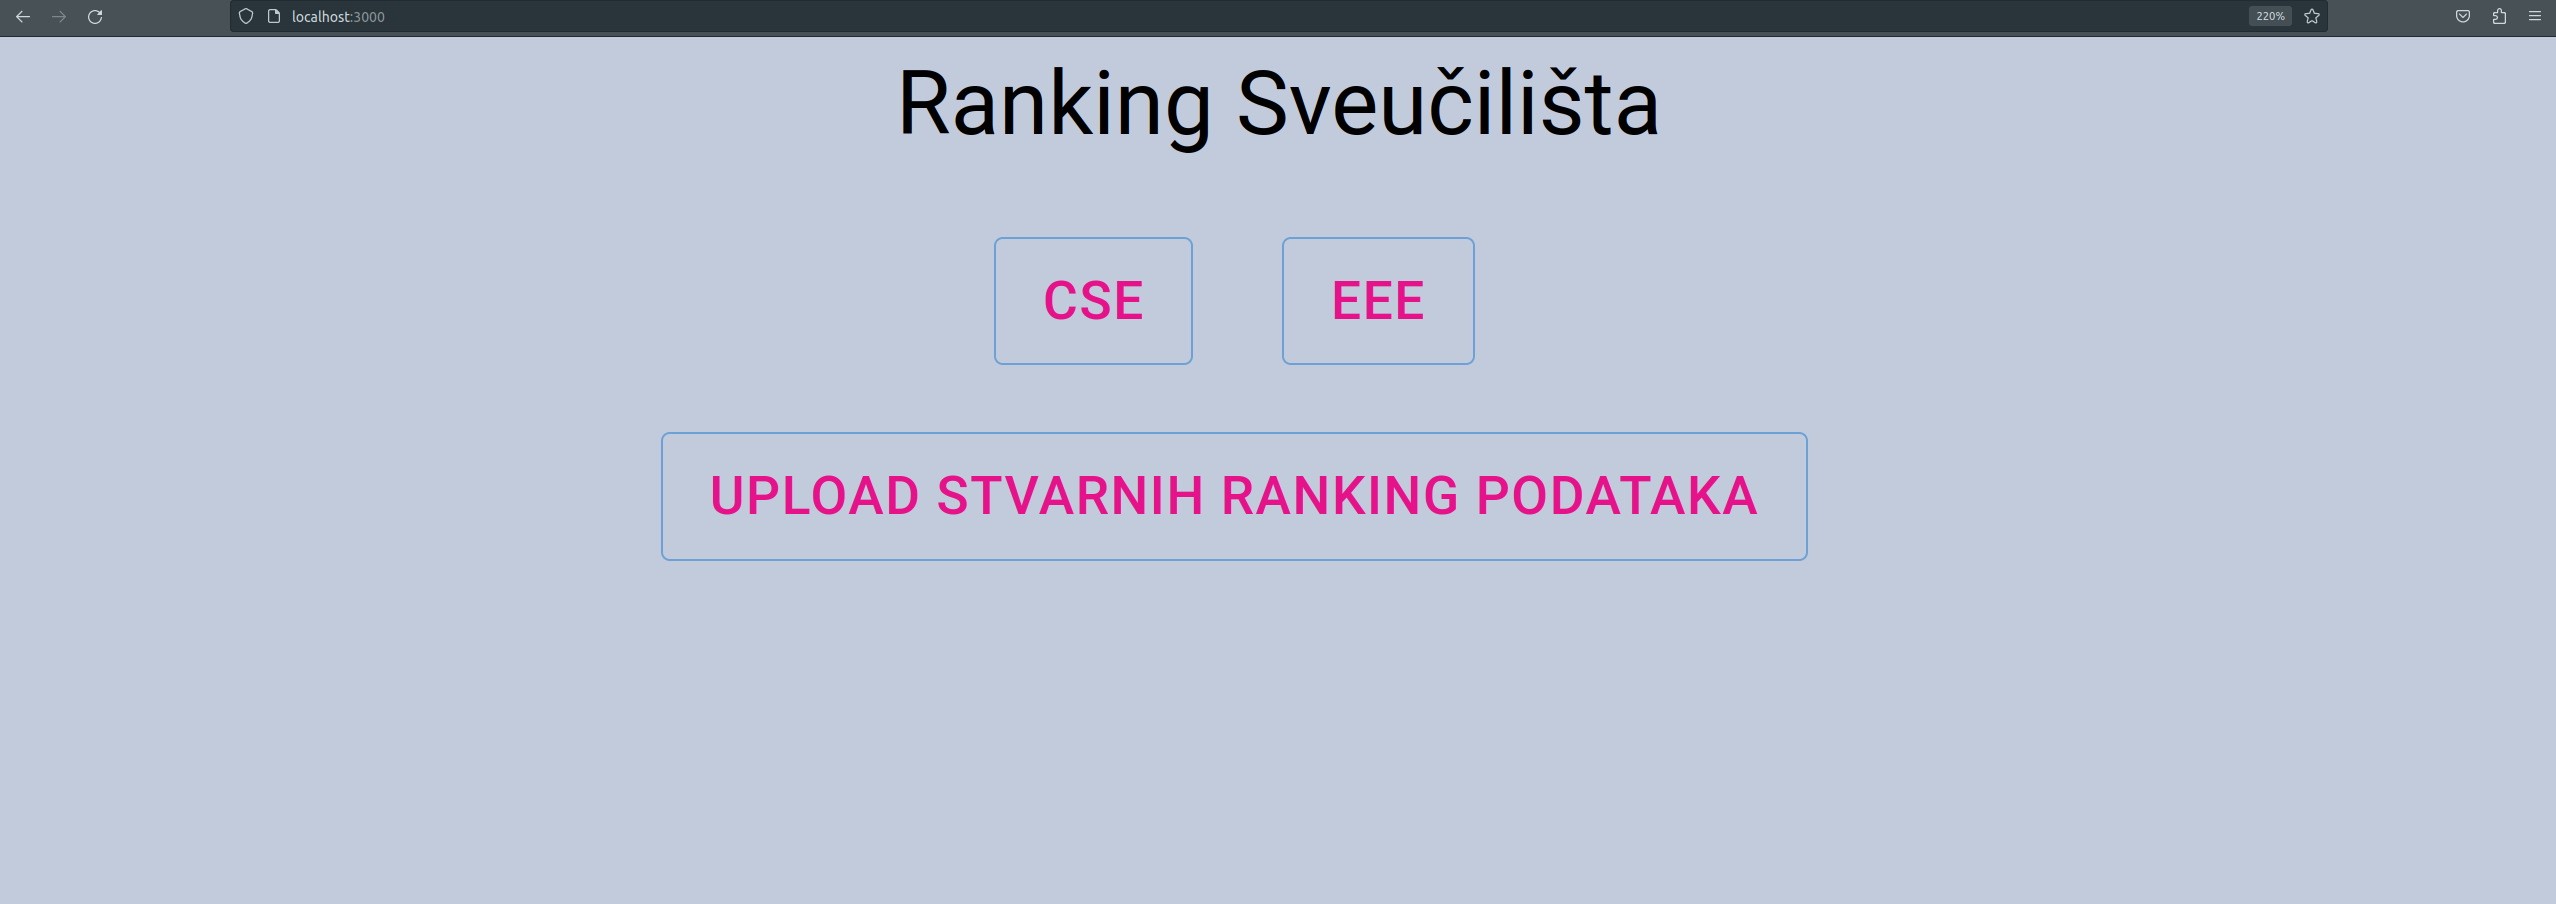
\includegraphics[scale=0.2]{homePage.png} 
    \caption{Prikaz početne stranice}
    \label{fig:homepage}
    \end{figure}
Početna stranica nalazi se na putanji \url{/}. Na početnoj stranici korisnik može birati između tri opcije. Pritiskom na neki od gornja dva gumba \emph{CSE} ili \emph{EEE}
korisnika će se preusmjeriti na stranicu za pregled procjene Shanghai Rankinga i svih vrijednosti indikatora za područje CSE, odnosno EEE.        
Pritiskom na donji gumb \emph{UPLOAD STVARNIH RANKING PODATAKA} korisnik će biti preusmjeren na stranicu na kojoj može objaviti .xlsx datoteku koja ima 
identične vrijednosti indikatora i pozicija za pojedina sveučilišta kao i Shanghai Ranking stranica.
\newpage\section{Tablični prikaz rang liste sveučilišta}
\begin{figure}[htb]
    \hspace*{-2cm}  
    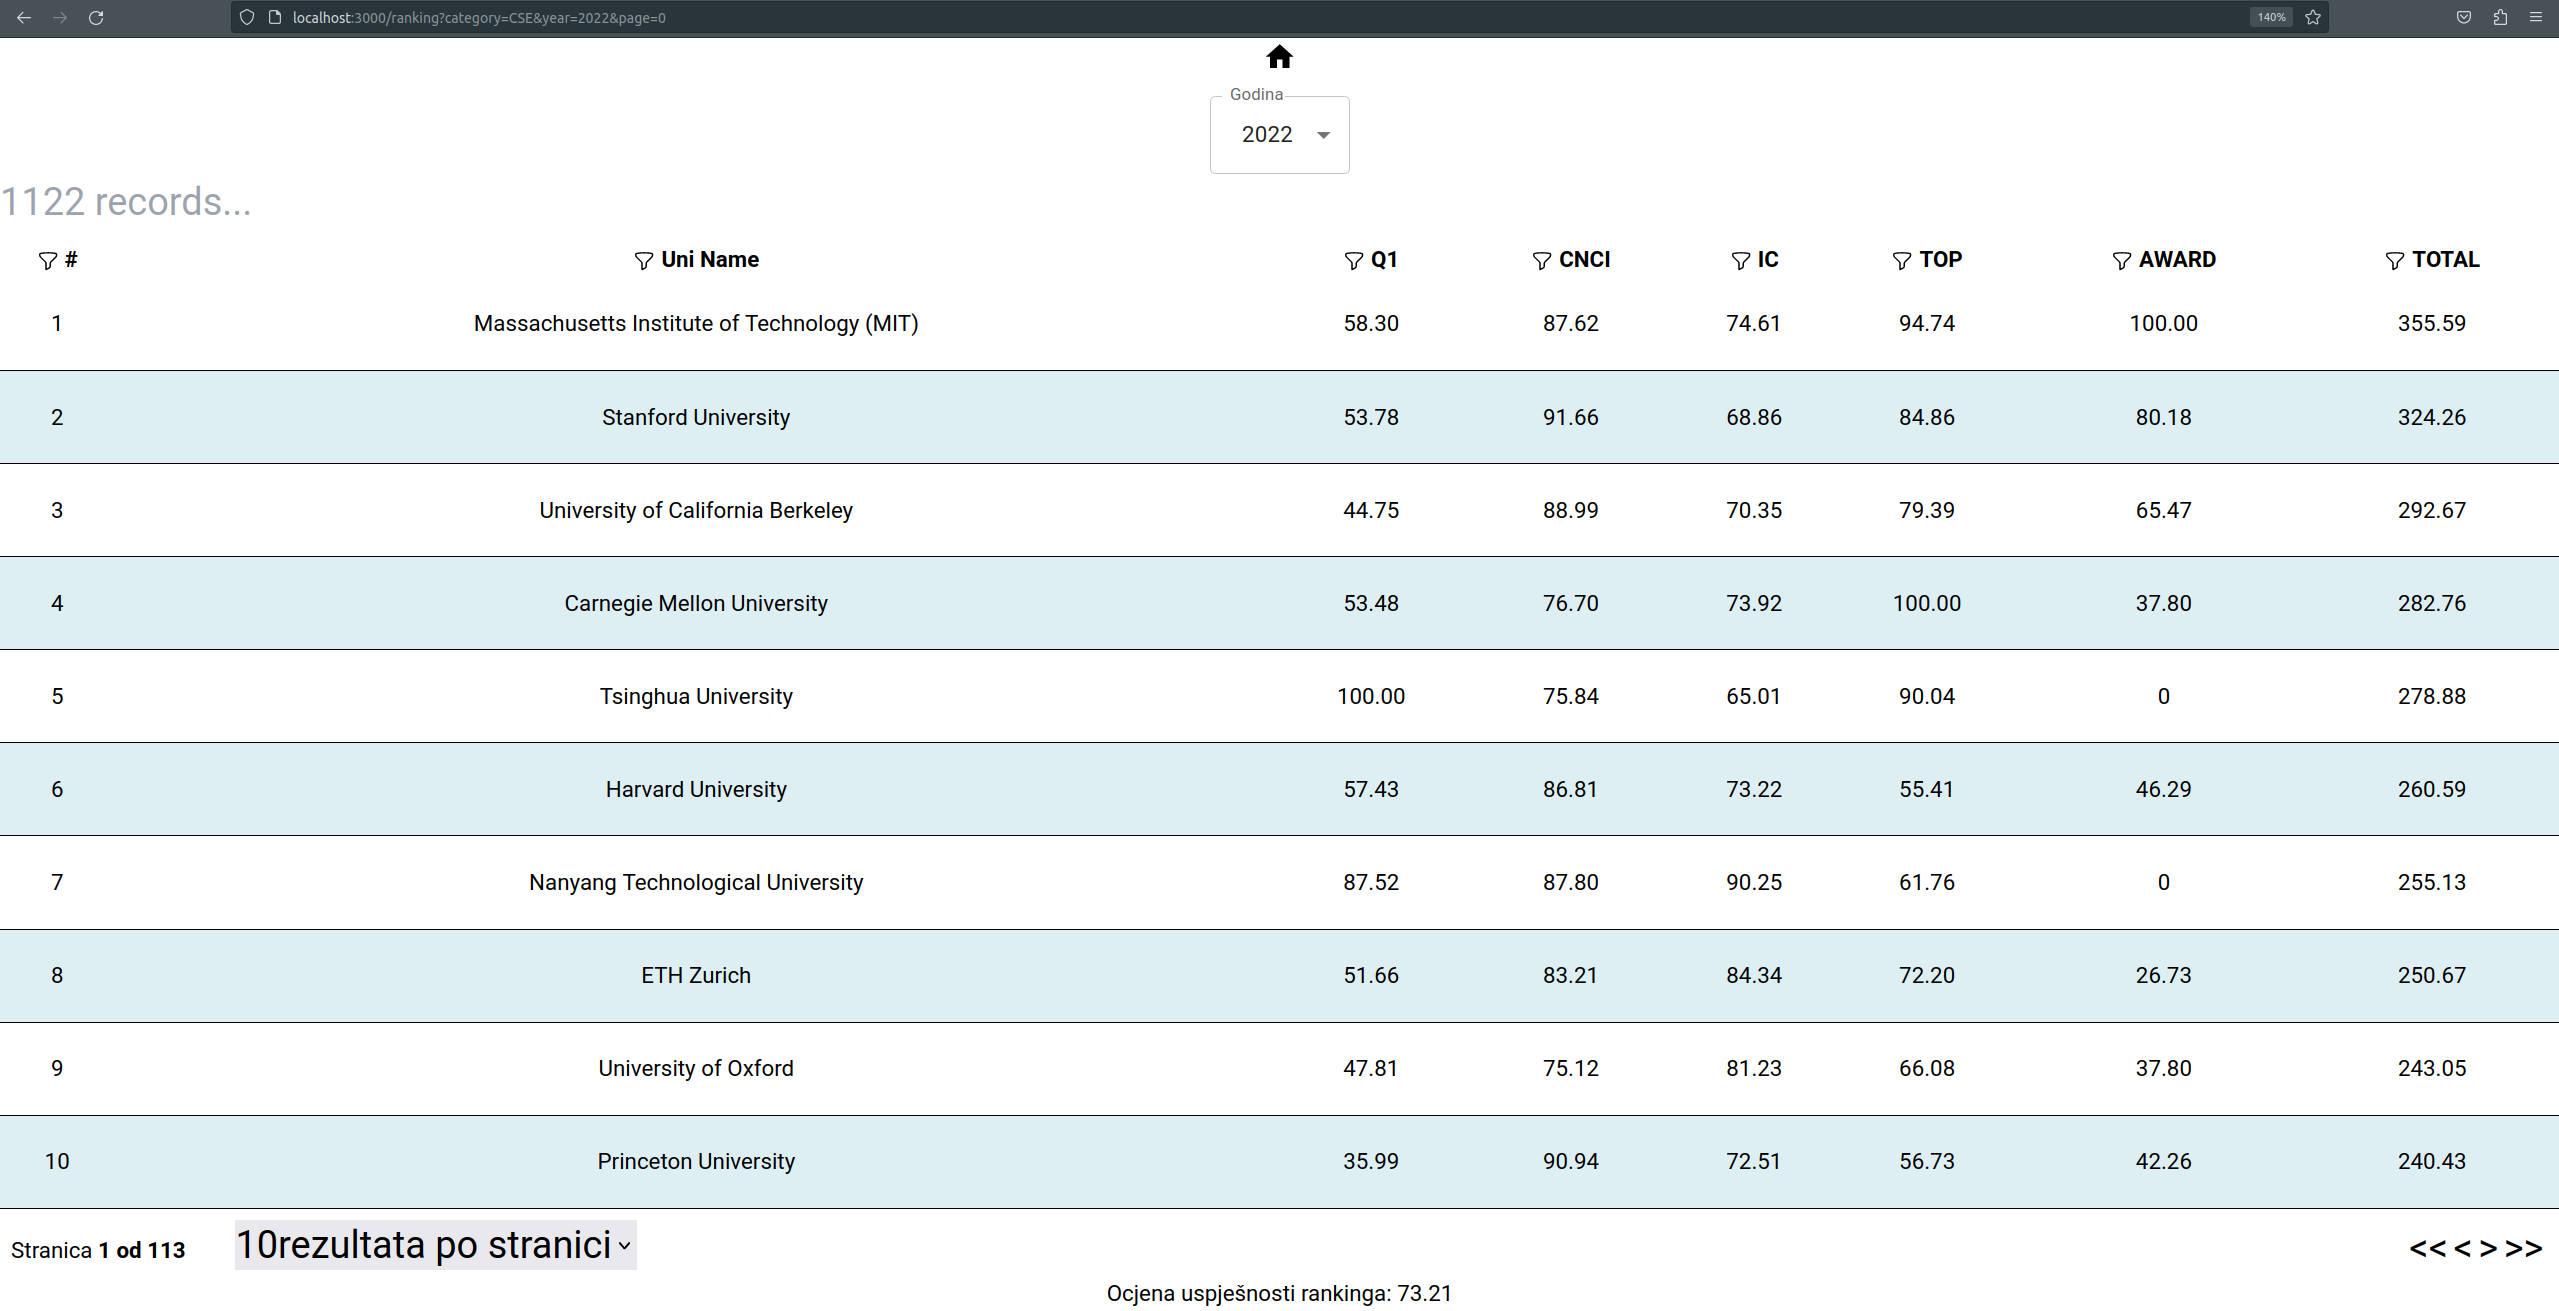
\includegraphics[scale=0.2]{tablica.png} 
    \caption{Procijenjena rang lista za područje CSE u 2022. godini}
    \label{fig:tablica}
    \end{figure}

Pritiskom na neki od gumba \emph{CSE} ili \emph{EEE} korisniku se prikaže stranica na slici \ref{fig:tablica}. Putanja koja vodi do ove stranice 
je \url{/ranking?category=CSE\&year=2022\&page=0}.
URL parametar \emph{category} specificira za koje područje se prikazuje rang lista, parametar \emph{year} specificira
za koju godinu se gleda rang lista, a parametar \emph{page} je pomoćni parametar za ostvarenje paginacije.  
U ovom konkretnom primjeru iz URL-a se vidi da korisnik trenutno gleda prvu stranicu (indeksiranje stranica kreće od 0) rang liste sveučilišta u području CSE za 2022.godinu.
\\Stranica na vrhu ima ikonu u obliku kućice s kojom se korisnik vraća na početnu stranicu. \\Odmah ispod ikone kućice nalazi se komponenta
za odabir godine za koju korisnik želi pogledati rang listu sveučilišta. Pritiskom na tu komponentu prikazuje se padajući izbornik 
s popisom godina od 2017. godine do trenutne godine. 
\begin{figure}[htb]
    \centering
       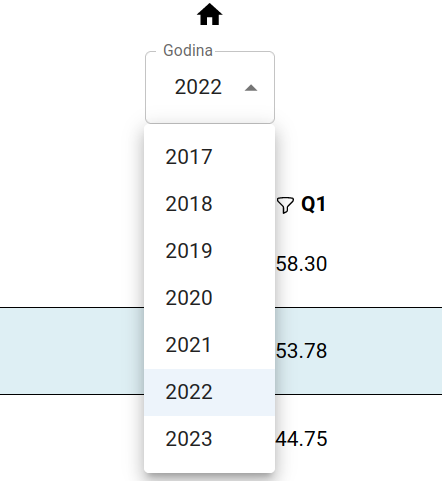
\includegraphics[scale=0.24]{select.png} 
       \caption{Komponenta za odabir godine rang liste sveučilišta}
       \label{fig:select}
       \end{figure}
Početna godina je 2017. jer od te godine su dostupne rang liste na stranici 
Shanghai Ranking. Kada korisnik odabere jednu od ponuđenih godina u URL-u se mijenja parametar \emph{year}, šalje se HTTP GET zahtjev na
poslužitelj te se ažurira tablica rang liste s podatcima za odabranu godinu koje poslužitelj pošalje u HTTP odgovoru \engl{response}.
\newpage Ispod komponente za odabir godine, a prije tablice rangiranja,
nalazi se polje za pretragu sveučilišta po njihovom imenu. Prije nego što korisnik krene upisivati slova u to polje, u njemu kao zamjenski tekst \engl{placeholder}
piše koliko sveučilišta se određene godine u nekom području našlo na procijenjenoj rang listi. Na slici \ref{fig:tablica} se vidi da je za 2022. godinu u području CSE 
na procijenjenoj rang listi 1122 sveučilišta.
Upisom imena sveučilišta na rang listi pojavit će se podatci samo za ona sveučilišta
koja u imenu sadrže podniz koji je korisnik upisao u polje za pretragu. Upisom podniza na poslužitelj HTTP GET zahtjevom šalje se taj podniz te se 
pretražuje baza podataka procjene rangiranja za određenu godinu u nekom području po imenu sveučilišta. Dolaskom HTTP odgovora ažuriraju se podatci u tablici.\\
\begin{figure}[htb]
    \hspace*{-2cm}  
       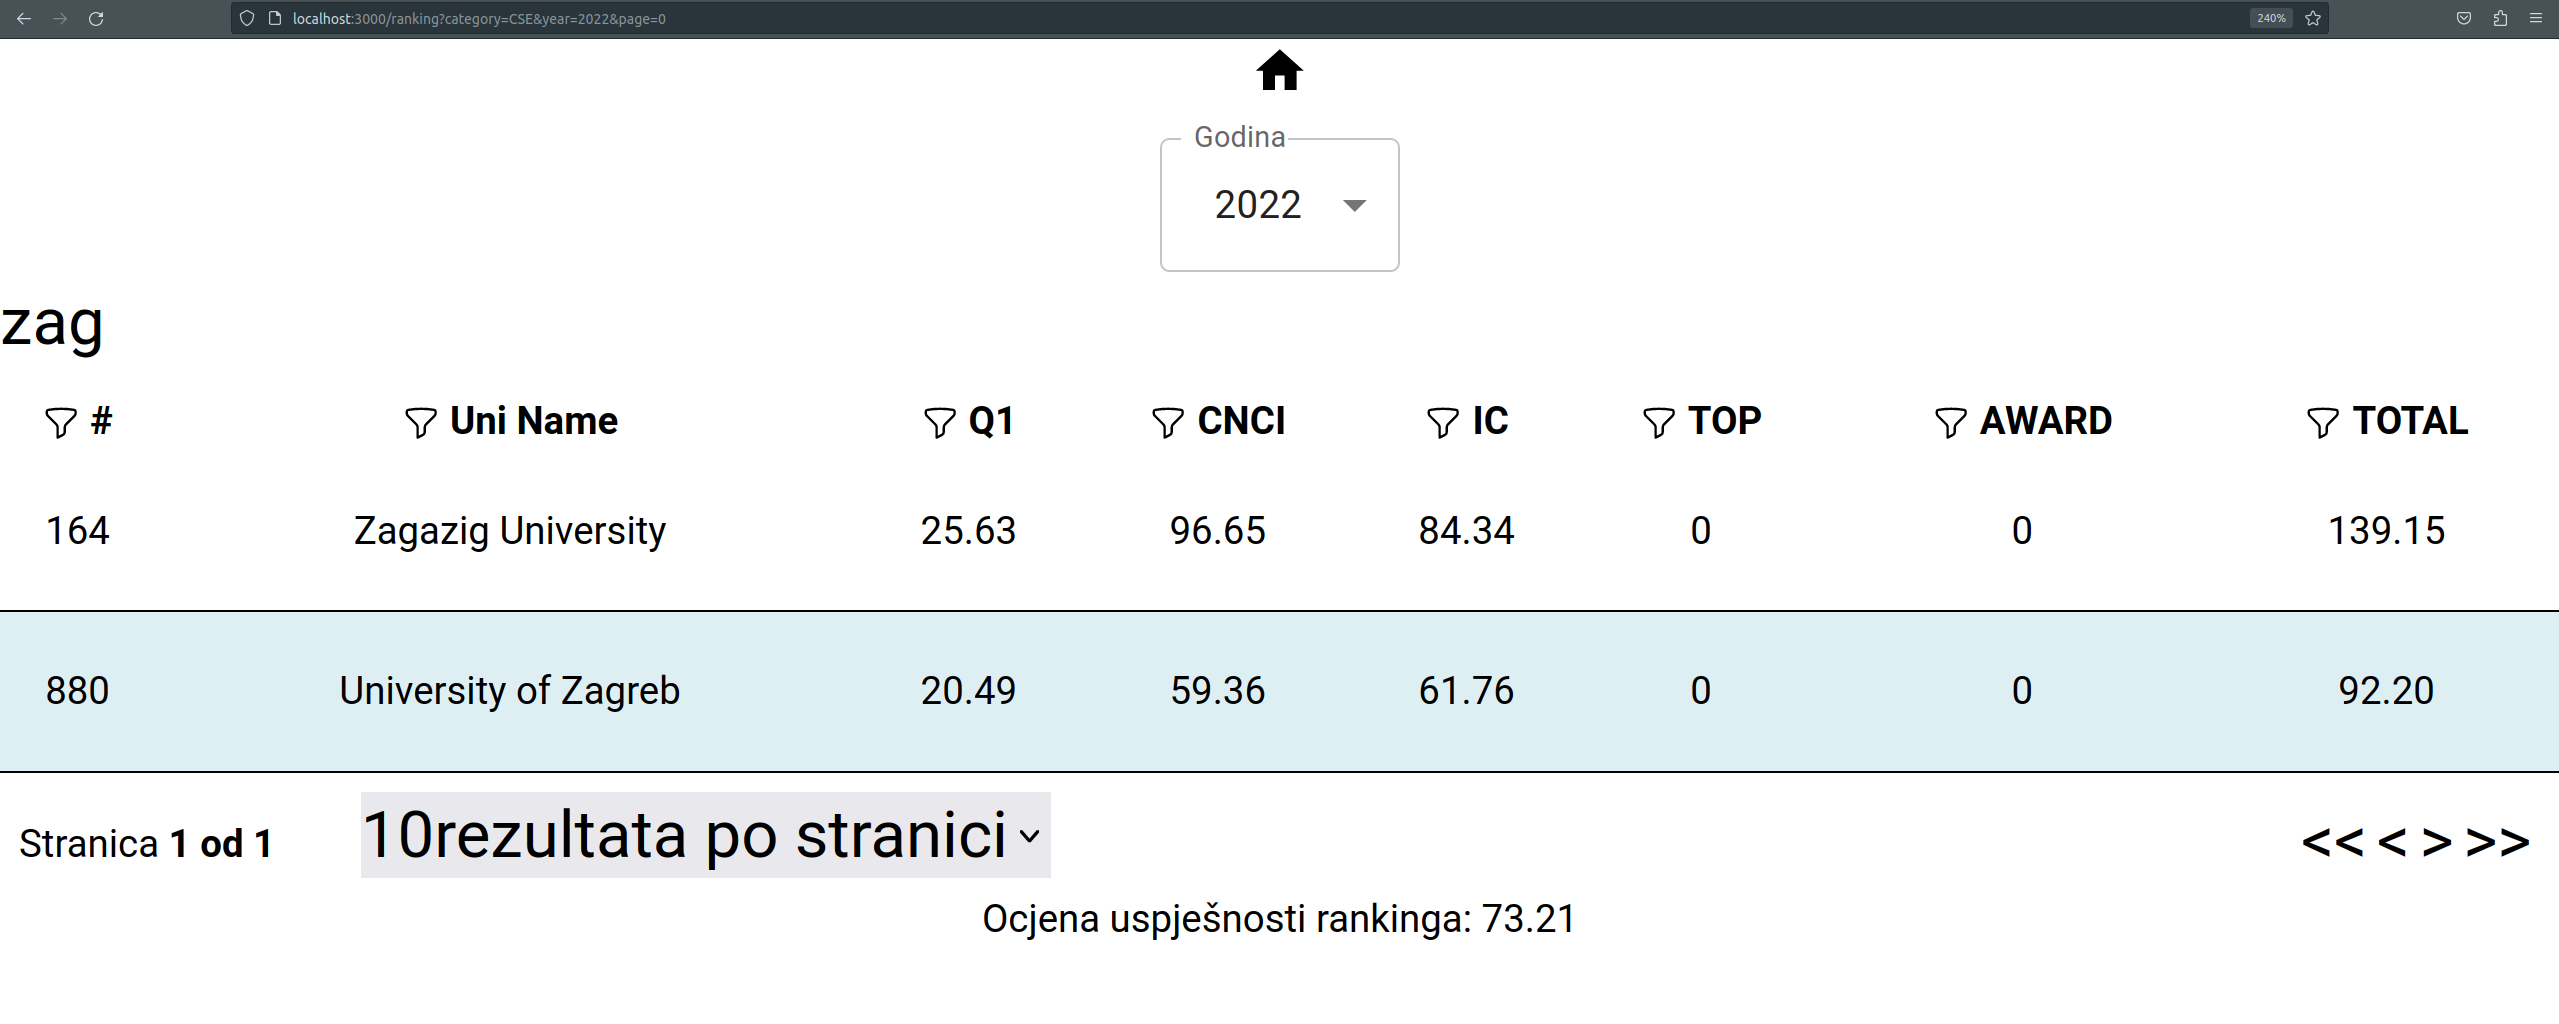
\includegraphics[scale=0.21]{search.png} 
       \caption{Primjer pretrage sveučilišta po imenu}
       \label{fig:search}
       \end{figure}
\\Na slici \ref{fig:search} se vidi primjer pretrage sveučilišta po imenu. Korisnik je upisao niz slova "zag" te se u tablici vide podatci za dva sveučilišta
koja u svom imenu sadrže navedeni podniz. 
\\Tablica rangiranja sastoji se od 8 stupaca. Zaglavlje tablice sadrži nazive vrijednosti koje se nalaze u pojedinim stupcima.
Prvi stupac pokazuje poziciju sveučilišta na rang listi za određenu godinu te u nekom području, drugi 
pokazuje ime sveučilišta, sljedećih pet stupaca sadrže vrijednosti koje se vežu uz indikatore Q1, CNCI, IC, \emph{Top} i \emph{Award}, a zadnji stupac sadrži ukupan rezultat sveučilišta 
u određenoj godini za neko područje prema kojem su sveučilišta sortirana i zove se Total. U zaglavlju tablice prije samog naziva vrijednosti stupca nalazi se ikona koja simbolizira
sortiranje tablice rangiranja. Ova funkcionalnost omogućena je za sve stupce osim prva dva. Ako korisnik pritisne na tu ikonu ili naziv stupca cijela tablica 
procjene rangiranja sortirat će se prema \\vrijednosti tog stupca silazno, odnosno uzlazno. 
\begin{figure}[htb]
    \hspace*{-2cm}  
       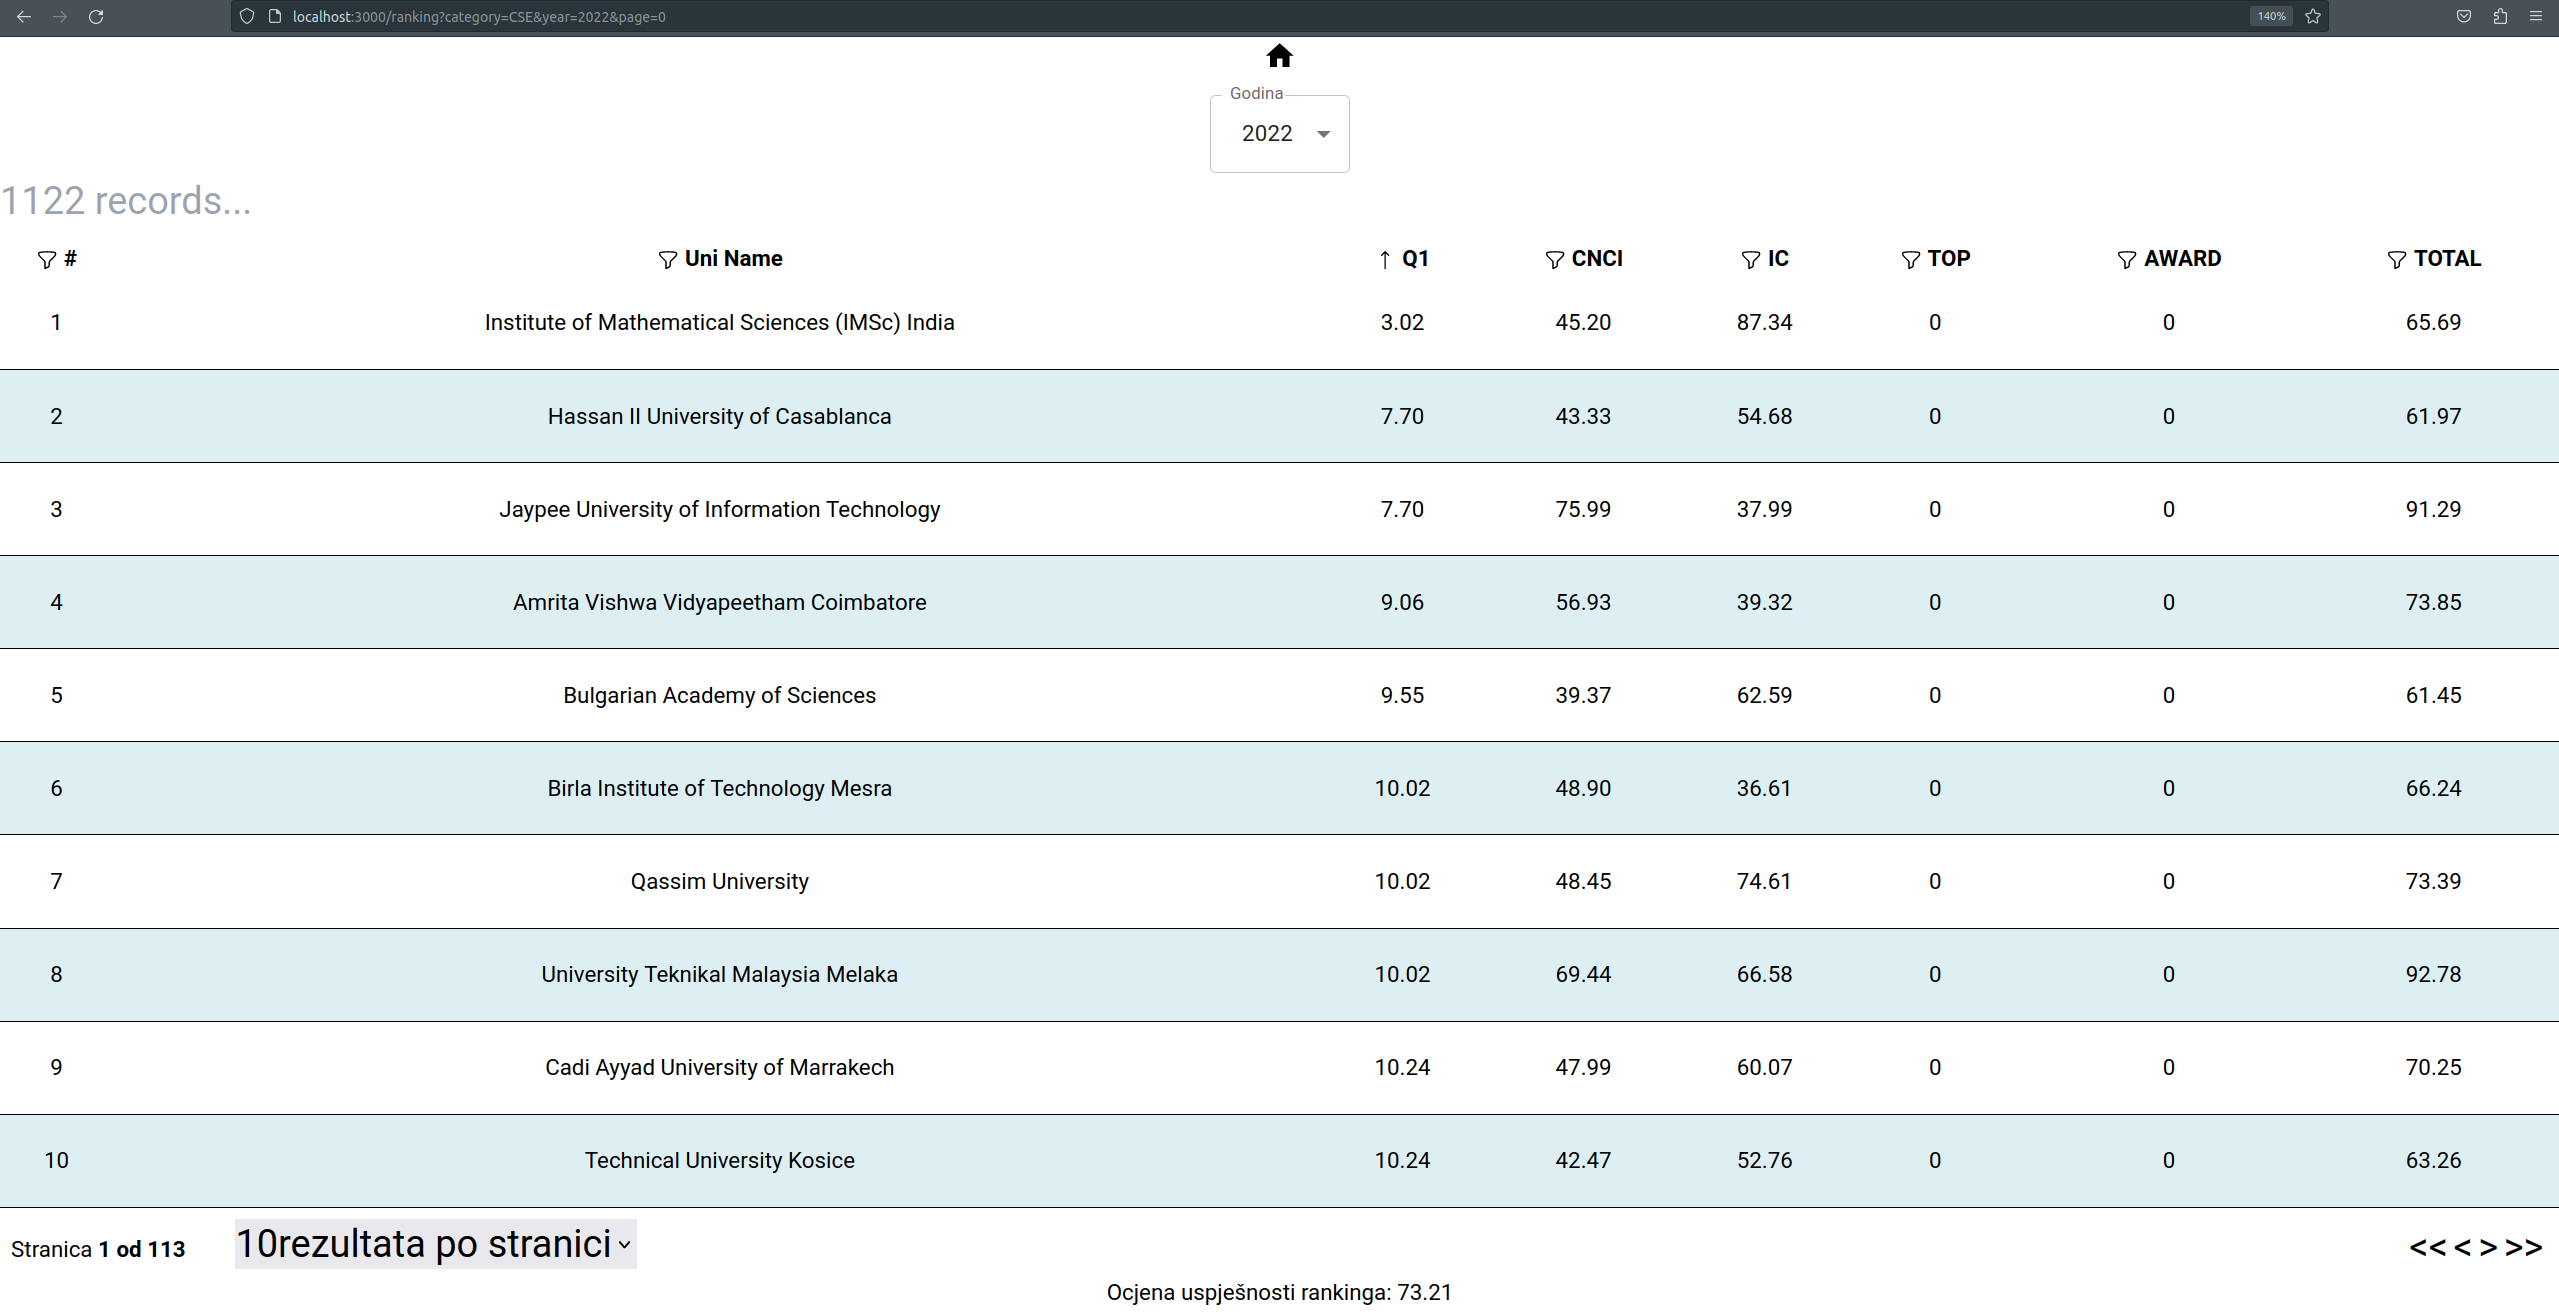
\includegraphics[scale=0.21]{sort1.png} 
       \caption{Primjer uzlaznog sortiranja rang liste prema vrijednosti indikatora Q1}
       \label{fig:sort1}
       \end{figure}
\\Slika \ref{fig:sort1} prikazuje stanje tablice nakon što je korisnik pritisnuo u zaglavlju tablice treći stupac koji ima naziv Q1. Sada se ikona koja simbolizira
sortiranje zamijenila s ikonom strelice koja pokazuje prema gore. Strelica prema gore simbolizira da se cijela rang lista
sortira uzlazno prema vrijednosti indikatora uz koji se nalazi strelica, u ovom slučaju to je indikator Q1. Sada su se podatci u tablici 
ažurirali te su sveučilišta sortirana uzlazno po vrijednosti indikatora Q1 što se i vidi u samoj tablici na slici \ref{fig:sort1} jer vrijednost indikatora Q1 za prvo 
sveučilište je 3.02, a za svako sljedeće sveučilište ta vrijednost je veća u odnosu na prethodno sveučilište. Sortiranje se može raditi i silazno. Tada se ikona promijeni
u strelicu koja je okrenuta prema dolje. Promjene \\vrste sortiranja između silaznog, uzlaznog ili zadanog \engl{default} se radi \\uzastopnim pritiskanjem 
jednog od zadnjih 6 stupaca u zaglavlju tablice.
\\\emph{Default} sortiranje je silazno prema vrijednosti stupca Total jer se tako dobije rang lista sveučilišta od najboljih prema najgorim uzimajući u obzir sve 
vrijednosti koje se vežu uz pojedine indikatore.
Istodobno sortiranje sveučilišta prema više vrijednosti stupaca nije moguće. Tako na primjer ako korisnik prvo odabere uzlazno sortiranje prema vrijednosti stupca 
Q1 te zatim odabere sortiranje za stupac IC, sortiranje prema \\vrijednosti stupca Q1 će se poništiti te će se primijeniti željeno sortiranje prema \\vrijednosti stupca IC.
Sortiranje sveučilišta se također odvija na 
poslužitelju, a parametri se prenose u sklopu HTTP GET zahtjeva. Dolaskom HTTP odgovora ažuriraju se podatci u tablici.
\\Zbog potencijalno velikog broja sveučilišta na rang listama, korisniku se ne prikažu sva sveučilišta u obliku jedne velike tablice nego 
je napravljena paginacija tako da se na jednoj stranici prikaže samo određeni broj zapisa iz rang liste sveučilišta. Informacija o tome na kojoj je trenutno stranici i 
koliko ukupno stranica rang liste ima korisniku je vidljiva ispod tablice uz lijevi rub. 
\begin{figure}[htb]
    \centering
       
\includegraphics[scale=0.3]{stranica.png} 
       \caption{Prikaz trenutne stranice i ukupnog broja stranica rang liste}
       \label{fig:paginacija}
       \end{figure}
\\Korisnik također može birati količinu redaka tablice po jednoj stranici. Pritiskom na komponentu ispod tablice otvara se 
izbornik gdje korisnik može birati između 10, 20, 30, 40 ili 50 redaka tablice po jednoj stranici. \emph{Default} vrijednost je 10. Ova \\vrijednost zajedno s 
trenutnim brojem stranice prenose se kao parametri prilikom HTTP GET zahtjeva kako bi poslužitelj znao koliko zapisa i s kojim pomakom mora vratiti u 
HTTP odgovoru klijentu. Na ovaj način na klijentskoj strani pohranjeno je uvijek najviše 50 zapisa što pridonosi brzini korisničkog sučelja.
\begin{figure}[htb]
    \centering
       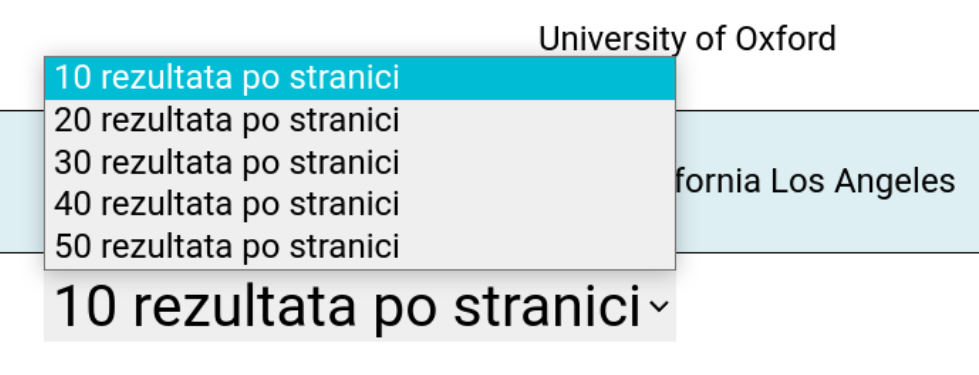
\includegraphics[scale=0.3]{brojstranica.png} 
       \caption{Odabir broja redaka tablice po jednoj stranici rang liste}
       \label{fig:brojstranica}
       \end{figure}
\\Ispod tablice rangiranja uz desni rub nalazi se područje za navigiranje stranicama rang liste.       
\begin{figure}[htb]
    \centering
       
\includegraphics[scale=0.4]{navigiranje.png} 
       \caption{Područje za navigiranje stranicama rang liste}
       \label{fig:navigacija}
       \end{figure}
Postoje četiri mogućnosti navigacije kao što se i vidi na slici \ref{fig:navigacija}. Pritiskom na ikonu označenu brojem 1 korisniku će se prikazati prva stranica rang liste.
Pritiskom na ikonu označenu brojem 2 korisnik će se pomaknuti za jednu stranicu unazad, a pritiskom na ikonu označenu brojem 3 prikazat će se sljedeća stranica. 
Pritisci na ikone 2 i 3 funkcioniraju ako uistinu postoji prethodna odnosno sljedeća stranica, u suprotnom se ništa ne događa.
Pritiskom na zadnju ikonu označenu rednim brojem 4 korisniku će se prikazati zadnja stranica rang liste. 
\\Ako je korisnik recimo navigirao na petu stranicu rang liste te u tom trenutku krenuo pretraživati sveučilišta, automatski ga se navigira na prvu stranicu rang liste.
\\Prilikom ažuriranja prikaza tablice rangiranja ne dolazi do ponovnog učitavanja stranice što je jedna od opisanih koristi jednostraničnih aplikacija.
\\Za vrijeme čekanja HTTP odgovora od poslužitelja korisniku se prikaže \\odgovarajuća ikona koja simbolizira učitavanje podataka te se pozadina posivi.
\begin{figure}[htb]
    \hspace*{-2cm}  
       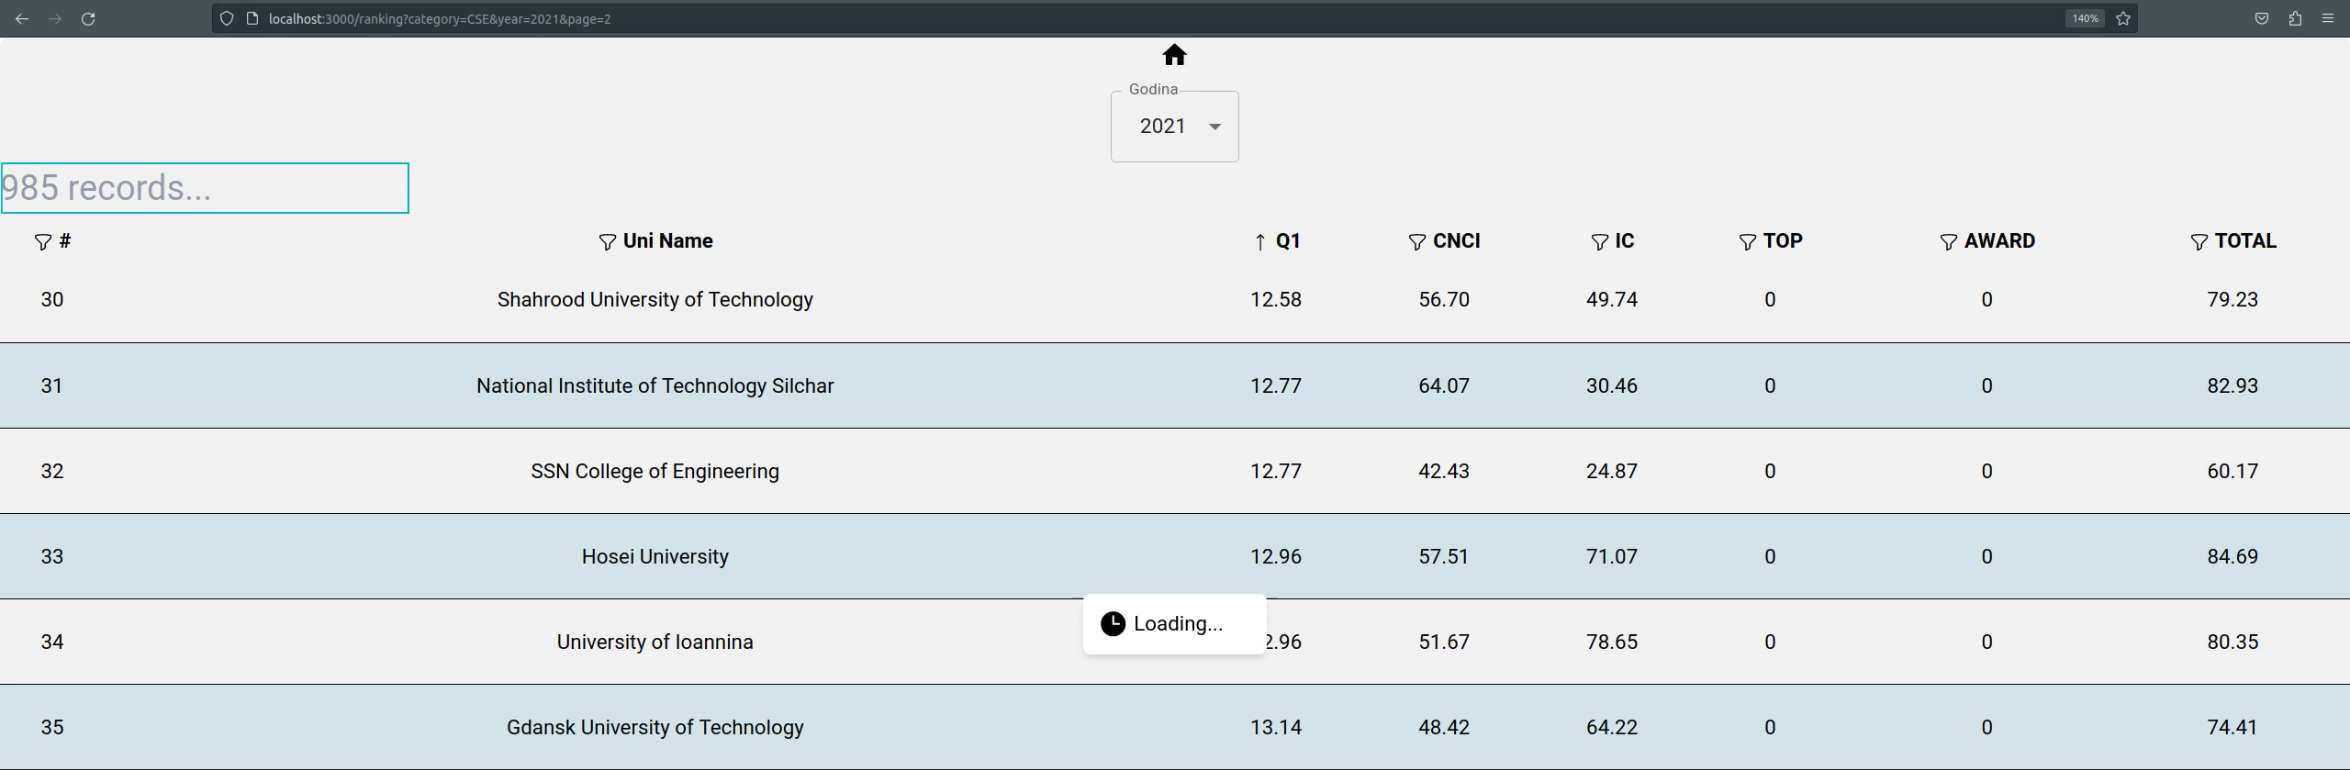
\includegraphics[scale=0.21]{loading.png} 
       \caption{Primjer čekanja HTTP odgovora poslužitelja}
       \label{fig:sort2}
       \end{figure}
\\Na svako ime sveučilišta u tablici rangiranja korisnik može pritisnuti mišem te će ga se preusmjeriti na stranicu s detaljnijim podatcima za to konkretno sveučilište.
\section{Stranica sveučilišta}
\label{section:unipagesection}
Temeljni funkcionalni zahtjevi nalažu da korisnik može pratiti rang sveučilišta i promjene vrijednosti indikatora tijekom godina, pogledati procjenu 
ranga sveučilišta u tekućoj godini te usporediti procijenjene vrijednosti indikatora sa stvarnim \\vrijednostima na stranici Shanghai Ranking. Ova stranica 
nudi te funkcionalnosti korisniku u obliku grafičkog prikaza. 
\\
\begin{figure}[htb]
    \hspace*{-2cm}  
       
\includegraphics[scale=0.21]{unipage.png} 
       \caption{Stranica sveučilišta}
       \label{fig:unipage}
       \end{figure}
\\Nakon što je korisnik pritisnuo ime nekog sveučilišta prikazat će mu se stranica na slici \ref{fig:unipage}. Stranica sa slike nalazi se na putanji 
\url{/rankingUni?uni=Massachusetts\%20Institute\%20of\%20Technology\%20(MIT)\&category=CSE}. Parametar \emph{uni} specificira za koje sveučilište će se prikazivati podatci, a 
parametar \emph{category} specificira za koje područje se prikazuju podatci. U primjeru sa slike \ref{fig:unipage} prikazana je stranica koja se odnosi na sveučilište 
Massachusetts Institute of Technology (MIT) za područje CSE. Područje za koje se promatraju podatci ovisi o tome za koje područje je korisnik prethodno gledao 
rang listu te se ono prenosi na ovu stranicu. 
\\Na ovoj stranici korisnik može birati između 3 ponuđene opcije. 
\\Pritiskom na prvi padajući izbornik prikazat će se grafički prikaz promjene vrijednosti indikatora
od 2017. godine, što se vidi na slici \ref{fig:unipage1}. 
\begin{figure}[htb]
    \centering
       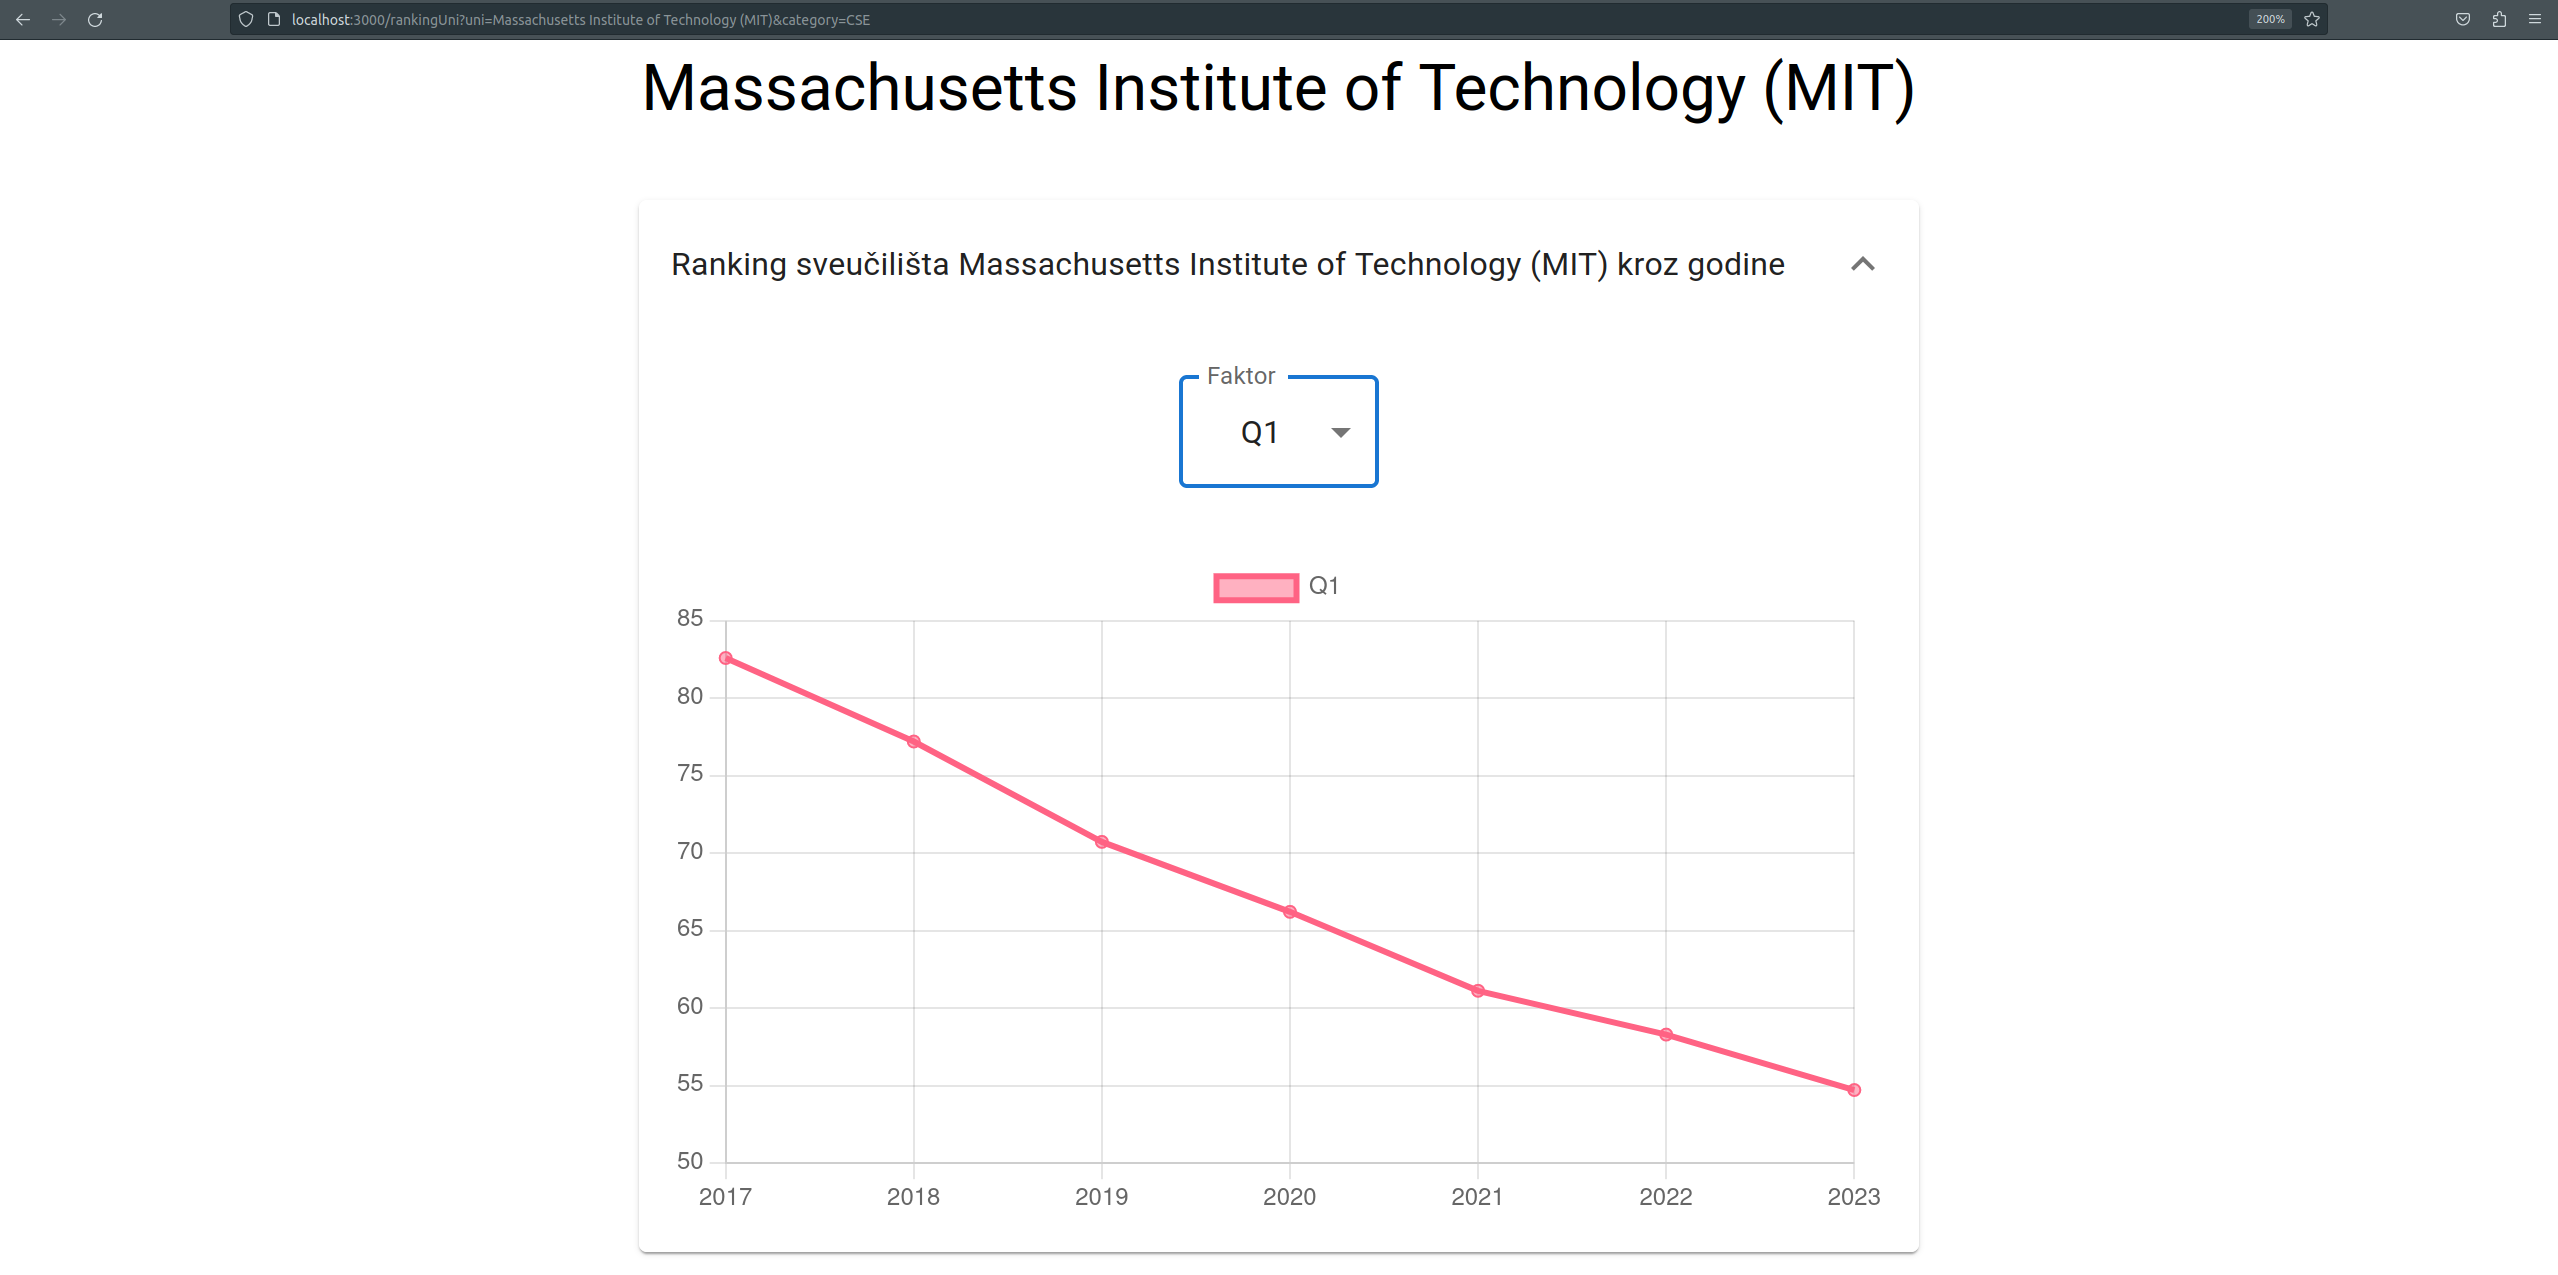
\includegraphics[scale=0.17]{uni1.png} 
       \caption{Grafički prikaz promjene vrijednosti indikatora}
       \label{fig:unipage1}
       \end{figure}
       
Ako korisnika zanima vrijednost nekog drugog indikatora, na raspolaganju mu je izbornik 
koji se nalazi iznad grafa prikazanog na slici \ref{fig:unipage1}. Postoji mogućnost pregleda promjene vrijednosti svih indikatora koji služe za računanje ranga: Q1, CNCI, IC, \emph{Top}, \emph{Award}. 
Promjene vrijednosti indikatora mogu se gledati posebno za svaki \\indikator ili za sve indikatore zajedno kako je prikazano na slici \ref{fig:svi}.
\begin{figure}[htb]
    \centering
       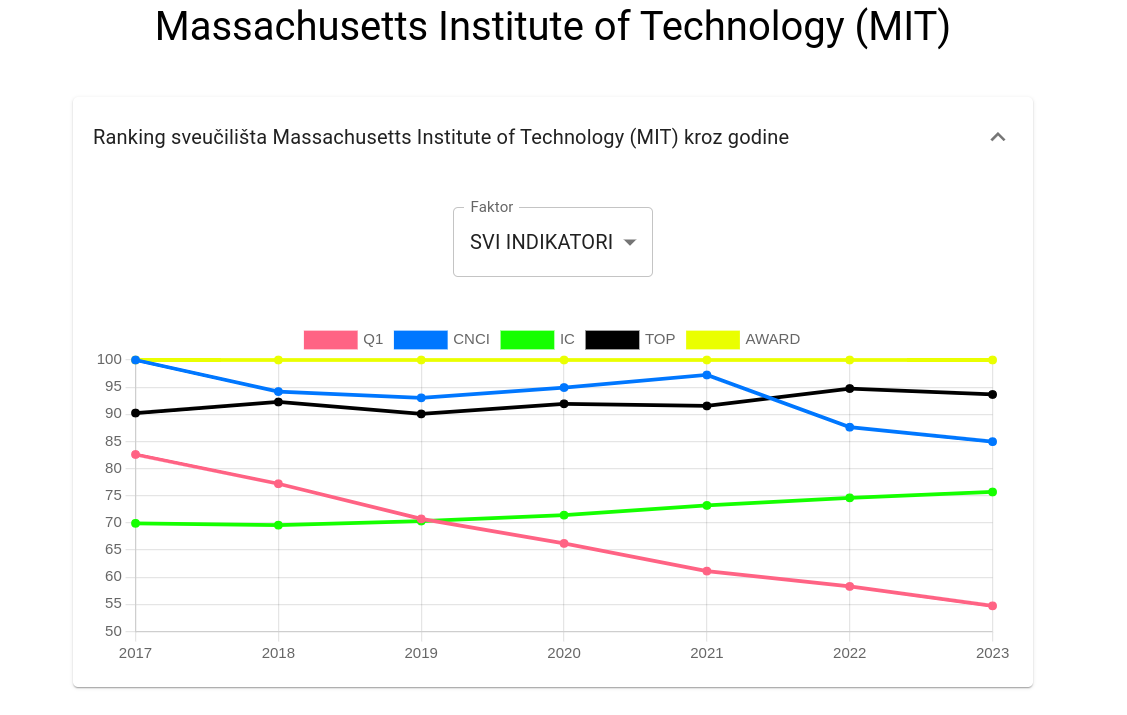
\includegraphics[scale=0.3]{svi.png} 
       \caption{Grafički prikaz promjene vrijednosti svih indikatora}
       \label{fig:svi}
       \end{figure}
\\Osim vrijednosti indikatora može se promatrati kako se pozicija \engl{position} sveučilišta te ukupna vrijednost \engl{total} prema kojoj se sveučilišta 
sortiraju na rang listi mijenjala kroz godine. Iz grafičkog prikaza se ne mogu potpuno točno pročitati vrijednosti podataka za neku godinu. Točan iznos 
nekog podatka za određenu godinu dobije se zadržavanjem strelice miša na krivulji iznad određene godine.

Pritiskom na drugi padajući izbornik korisniku se prikaže isti graf s opcijom pregleda vrijednosti indikatora
kao i u prethodnom slučaju. Jedina razlika je što ovaj graf prikazan na slici \ref{fig:uni3}
prikazuje promjenu procijenjenih vrijednosti indikatora tijekom mjeseci tekuće godine. Primjer sa slike \ref{fig:uni3} nije reprezentativan jer su podatci 
prikupljani u kratkom vremenskom razdoblju, no kada bi se aplikacija držala pokrenutom tijekom jedne godine vidjele bi se promjene na grafu. Pregledom ovog 
grafa može se procijeniti kako će izgledati Shanghai Ranking rang lista za trenutnu godinu prije \\službene objave. 
\begin{figure}[htb]
    \hspace*{-2cm}  
       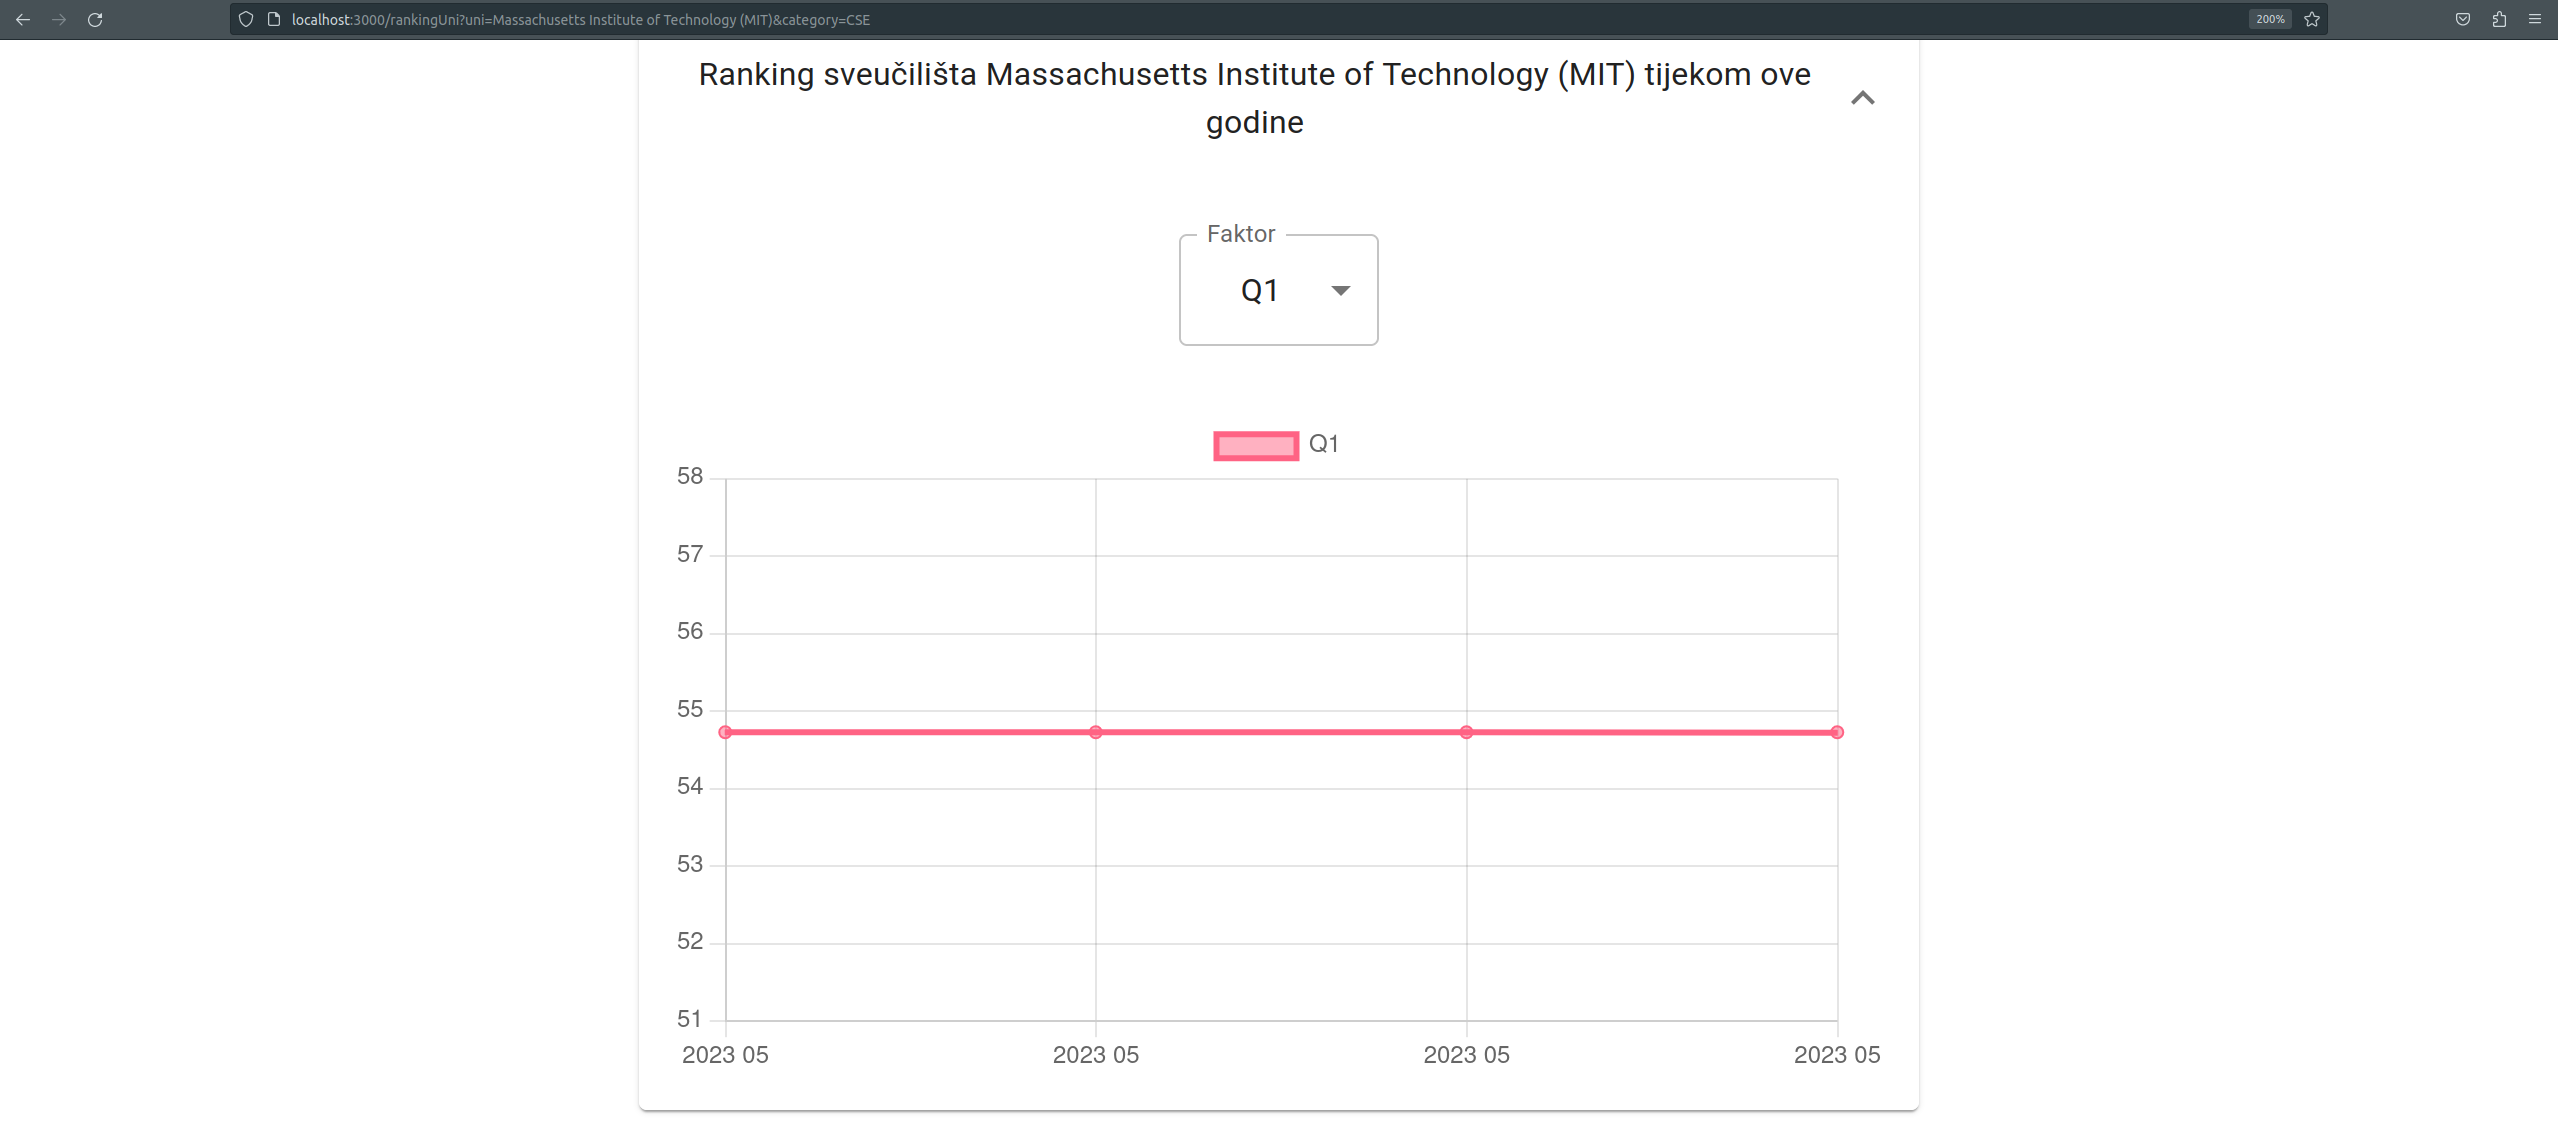
\includegraphics[scale=0.21]{uni3.png} 
       \caption{Prikaz vrijednosti indikatora za trenutnu godinu}
       \label{fig:uni3}
       \end{figure} 
\\\\Pritiskom na treći padajući izbornik prikaže se grafički prikaz na slici \ref{fig:uni4}. 
\begin{figure}[htb]
    \centering
       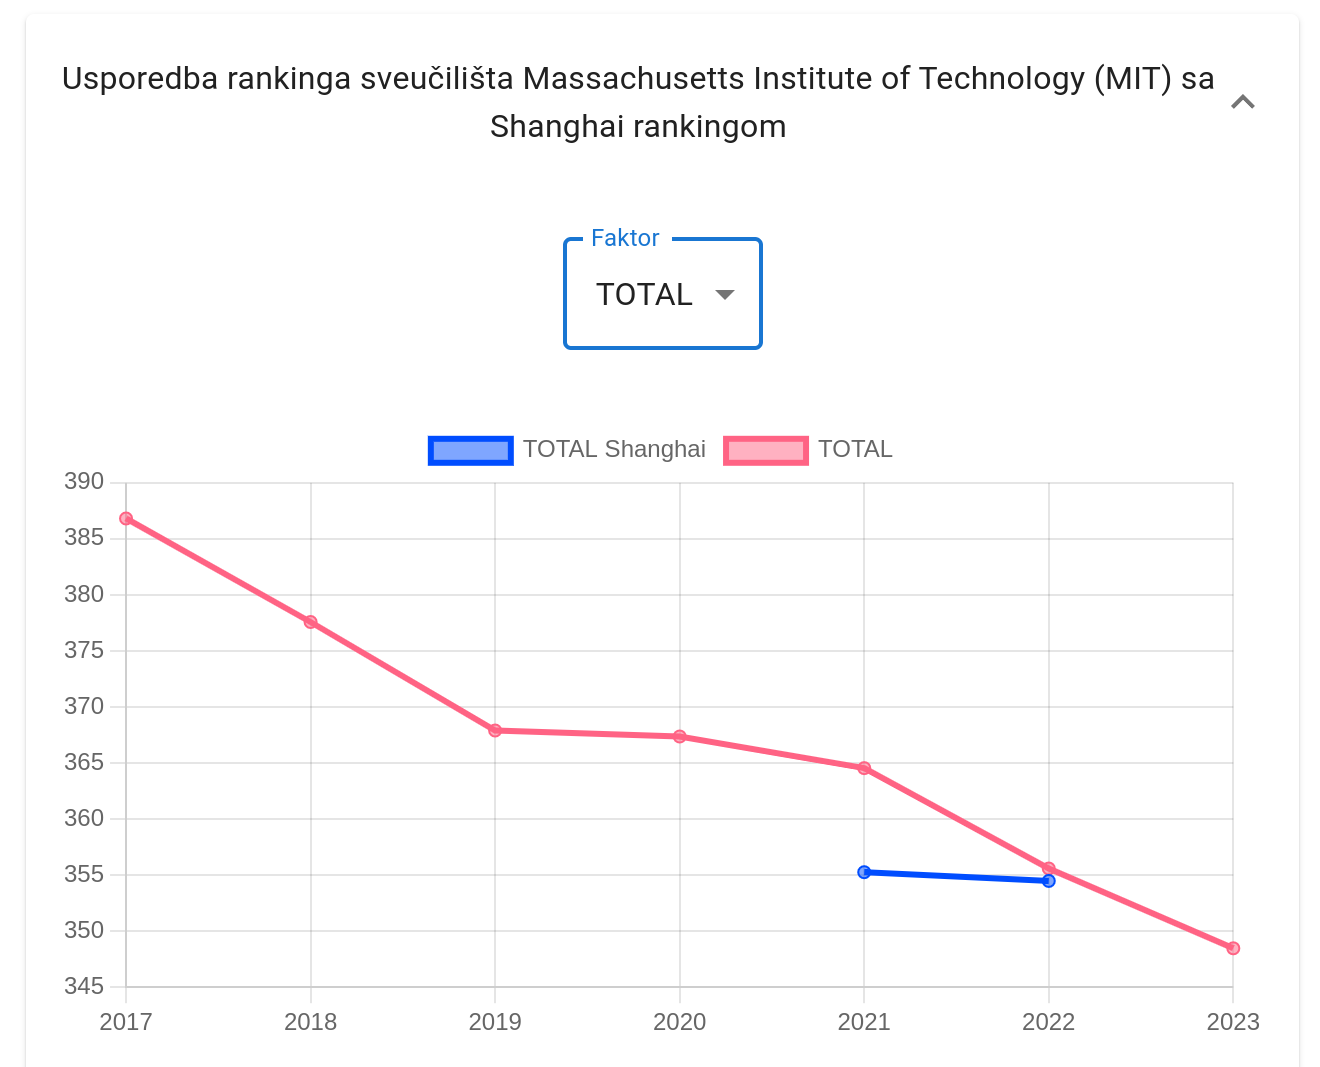
\includegraphics[scale=0.17]{uni4.png} 
       \caption{Grafički prikaz usporedbe procijenjenih i Shanghai Ranking vrijednosti indikatora}
       \label{fig:uni4}
       \end{figure} 
       \FloatBarrier
Na ovom grafu postoje dvije krivulje, ona označena plavom bojom predstavlja 
stvarne vrijednosti indikatora sa stranice Shanghai Ranking, dok ona označena crvenom bojom predstavlja procijenjene vrijednosti indikatora.
Na ovaj način može se lakše vizualno usporediti koliko je procjena vrijednosti indikatora i njihove ukupne sume \engl{total} prema kojoj se rangiraju sveučilišta dobra. 
Na ovom konkretnom primjeru vidi se odnos procijenjene i stvarne 
vrijednosti ukupne sume indikatora.
Podatke sa Shanghai Ranking stranice korisnik unosi postavljanjem \engl{upload} 
odgovarajuće .xlsx datoteke, što je opisano u sljedećem dijelu.
\\Svi podatci potrebni za prikaz grafova dohvaćaju se pomoću HTTP GET zahtjeva na poslužitelj. Na ovoj stranici, kao i prethodno opisanoj, 
vide se prednosti \\jednostraničnih aplikacija jer promjenom grafa ili vrijednosti koja se prikazuje na grafu ne dolazi do ponovnog 
učitavanja web stranice.

\section{Stranica za postavljanje podataka sa \\Shanghai Ranking stranice}
Usporedba procijenjenih i Shanghai Ranking vrijednosti indikatora moguća je \\postavljanjem .xlsx datoteke koja sadrži 
podatke sa Shanghai Ranking stranice. Kako korisnik ne bi morao direktno unositi podatke u bazu podataka, na ovoj stranici može kroz 
interaktivno sučelje postaviti datoteku sa Shanghai Ranking podatcima koji će se automatski upisati u odgovarajuću tablicu u bazi podataka.
\\Ova stranica prikazana je na slici \ref{fig:upload} i ima URL \url{/upload}.
\\Na stranici u gornjem dijelu postoje dvije komponente za odabir područja, koje može biti CSE ili EEE, i godine, koja se kreće od 2017. do trenutne. Nakon što 
se odaberu te dvije vrijednosti korisnik može pritisnuti gumb s tekstom "Postavi datoteku" nakon čega mu se otvara preglednik datoteka osobnog računala
u kojem može izabrati koju datoteku želi postaviti. Ako korisnik postavi datoteku koja nema .xlsx proširenje, ispisat će mu se poruka pogreške kao na 
slici \ref{fig:error}.
\begin{figure}[htb]
    \hspace*{-2cm}  
       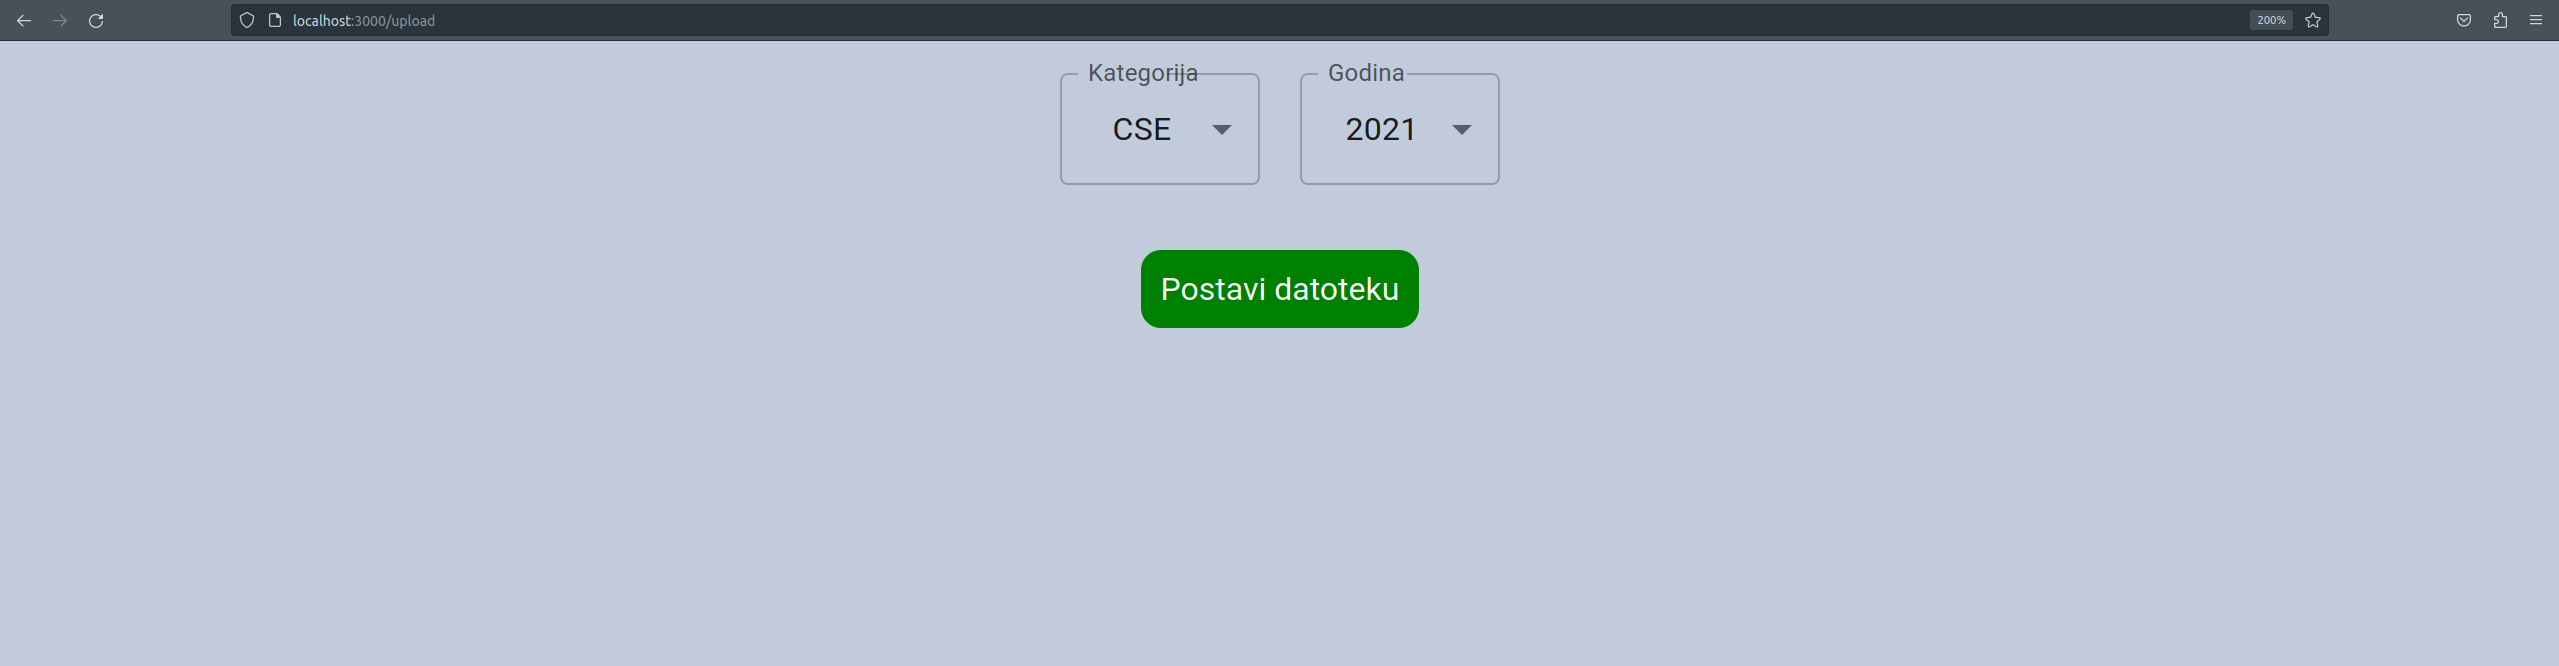
\includegraphics[scale=0.2]{upload.png} 
       \caption{Stranica za postavljanje stvarnih Shanghai Ranking podataka}
       \label{fig:upload}
       \end{figure} 
 \begin{figure}[htb]
        \centering
           
\includegraphics[scale=0.2]{error.png} 
           \caption{Poruka greške u slučaju postavljanja neispravne datoteke}
           \label{fig:error}
           \end{figure}        
\\Zapisi u postavljenoj datoteci trebaju biti formatirani na ispravan način kako bi se \\podatci uspješno unijeli u bazu podataka. 
Na slici \ref{fig:real} vidi se nekoliko zapisa ispravno formatirane .xlsx datoteke. Svaki redak zapisa treba imati sedam stupaca čiji su nazivi redom:
ime sveučilišta, vrijednost Q1, CNCI, IC, \emph{Top} i \emph{Award} indikatora te pozicija. Vrijednost podatka \emph{Total} prema kojem se sortiraju 
sveučilišta nije potrebno upisati jer se on lako izračuna iz zadanih vrijednosti indikatora. Pozicija sveučilišta se također mogla
izostaviti uz pretpostavku da će svaka postavljena datoteka imati zapise za sva sveučilišta za neku godinu u određenom području, ali
na ovaj način korisnik može unijeti samo nekoliko zapisa za sveučilišta koja su mu od interesa te dobiti mogućnost 
grafičke usporedbe podataka na stranici opisanoj u odjeljku \ref{section:unipagesection}.
\begin{figure}[htb]
    \hspace{-1.2cm} 
       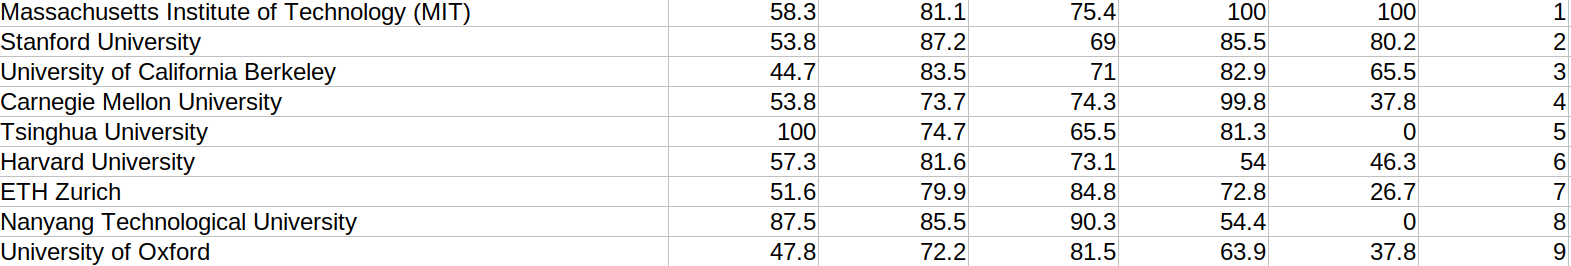
\includegraphics[scale=0.3]{real.png} 
       \caption{Prikaz zapisa datoteke sa stvarnim Shanghai Ranking podatcima za neku godinu u nekom području gdje su stupci redom: naziv sveučilišta, vrijednosti indikatora Q1, CNCI, IC, \emph{Top} i \emph{Award} te pozicija
       sveučilišta te godine na rang listi}
       \label{fig:real}
       \end{figure}  
\chapter{Prijedlozi za budući razvoj}
Aplikacija ima raznih mogućnosti napretka. Neki od mogućih nadogradnji su: dodavanje rang lista za druga područja istraživanja, 
dodavanje novog algoritma i indikatora za izračun rang liste te detaljnija 
statistička analiza vrijednosti indikatora pojedinog sveučilišta. 
\\Aplikacija trenutno nudi uvid samo u numeričke vrijednosti indikatora, a u nekoj sljedećoj nadogradnji bilo bi korisno dobiti uvid u popis radova i njihovih autora koji su utjecali na 
vrijednost indikatora. 
\\Osim rangiranja sveučilišta, može se dodati prikaz informacije o tome koliko pojedine obrazovne ustanove koje su dio sveučilišta pridonose rangu.
\chapter{Zaključak}
Procjena ranga sveučilišta omogućava uvid u kvalitetu nastave i profesora koji predaju na tom sveučilištu. Bez ikakve povratne informacije 
teško je zaposlenicima sveučilišta odrediti rade li dobar posao i što moraju popraviti kako bi im se reputacija poboljšala.
Shanghai Ranking lista djelomično rješava taj problem za neka sveučilišta. Problem Shanghai Ranking liste je što za određena područja ne nudi 
informacije o \\rangu sveučilišta ako nije u prvih 500 u svijetu. Ova aplikacija rješava taj problem te se na procijenjenoj rang listi nalaze sva sveučilišta 
za koja postoje podatci u InCites i WoS bazama. Dobro razumijevanje računanja vrijednosti indikatora bilo je ključno za ovu aplikaciju.
\\Odabir tehnologija Node.js, Express, React, Puppeteer PostgreSQL te ostalih bio je ispravan zbog velike količine dokumentacije i dostupne podrške. Ključni dijelovi 
ove aplikacije su bili ostvarenje periodičkog punjenja baze podataka s novim vrijednostima indikatora te izrada tablice rang liste i grafova za vizualni prikaz promjene vrijednosti indikatora kroz vrijeme. 
Procjena rang liste bila je jako uspješna za područje EEE te nešto manje za područje CSE.
Dodavanjem Docker podrške aplikacija je postala široko primjenjiva zbog jednostavnog postavljanja na bilo koji poslužitelj koji podržava Docker.

\bibliography{literatura}
\bibliographystyle{fer}
\nocite{*}


\begin{sazetak}
Završni rad razmatra izradu aplikacije za praćenje rangiranja sveučilišta u područjima \emph{Computer Science \& Engineering (CSE)} i 
\emph{Electrical \& Electronic Engineering (EEE)} prema algoritmu Shanghai Ranking sustava.
Aplikacija rješava problem \\nedostupnosti uvida u rang i vrijednosti indikatora za niže rangirana sveučilišta na stranici Shanghai Ranking te nudi praćenje procijenjenih vrijednosti indikatora i ranga za trenutnu godinu prije nego što 
izađe službena Shanghai Ranking rang lista. Korisniku nudi tablični prikaz procijenjene rang liste s vrijednostima indikatora koji se koriste za njezin izračun,
grafički prikaz promjene vrijednosti indikatora i ranga odabranog sveučilišta, usporedbu procijenjenog rangiranja sa Shanghai Ranking sustavom te pretragu baze podataka prema imenu sveučilišta.
Glavne tehnologije korištene za izradu aplikacije su: React, Node.js, Express.js, PostgreSQL, Puppeteer i Docker.


\kljucnerijeci{Shanghai Ranking, \emph{Computer Science \& Engineering (CSE)}, \emph{Electrical \& Electronic Engineering (EEE)}, Puppeteer, Node.js, Express, React, PostgreSQL, 
procjena rangiranja, Docker, grafički prikaz vrijednosti indikatora}
\end{sazetak}
\newpage
% TODO: Navedite naslov na engleskom jeziku.
\engtitle{An application for monitoring the ranking of universities according to the Shanghai List}
\begin{abstract}
Final work considers the creation of application for monitoring university rankings in the fields of Computer Science \& Engineering (CSE) and
Electrical \& Electronic \\Engineering (EEE) according to the Shanghai Ranking system algorithm.
The application solves the problem of the unavailability of ranking data for lower-ranked universities and offers monitoring of the ranking assessment for the current year before
the official Shanghai Ranking ranking list is out. It offers the user a tabular view of the estimated ranking along with the values of the indicators used to calculate the \\ranking,
graphical representation of changes in the ranking data of the selected university, comparison of the ranking assessment with the Shanghai Ranking data, and database search by university name.
The main technologies used to create the application are: React, Node.js, Express.js, PostgreSQL, Puppeteer and Docker.

\keywords{Shanghai Ranking, Computer Science \& Engineering (CSE), Electrical \& Electronic Engineering (EEE), Puppeteer, Node.js, Express, React, PostgreSQL, \\ranking assessment, Docker, graphic display of ranking data}
\end{abstract}

\end{document}
